%%%%%%%%%%%%%%%%%%%%%%%%%%%%%%%%%%%%%%%%%
% University of Hong Kong Masters/Doctoral Thesis 
% LaTeX Template
% Version 3.0 (01/07/2020)
% 
% Version 2.x major modifications by:
% Vel (vel@latextemplates.com)
% 
% This template is based on the template by:
% Steve Gunn (http://users.ecs.soton.ac.uk/srg/softwaretools/document/templates/)
% Sunil Patel (http://www.sunilpatel.co.uk/thesis-template/)
% Johannes Böttcher (http://www.latextemplates.com/template/masters-doctoral-thesis)
%
% Template license:
% CC BY-NC-ND 4.0 (https://creativecommons.org/licenses/by-nc-nd/4.0/)
%
% Author:  Nan Meng
% Contact: u3003637@connect.hku.hk
%
%%%%%%%%%%%%%%%%%%%%%%%%%%%%%%%%%%%%%%%%%


%----------------------------------------------------------------------------------------
%	PACKAGES AND OTHER DOCUMENT CONFIGURATIONS
%----------------------------------------------------------------------------------------

\documentclass[
10pt, % The default document font size, options: 10pt, 11pt, 12pt
%oneside, % Two side (alternating margins) for binding by default, uncomment to switch to one side
english, % ngerman for German
onehalfspacing, % Single line spacing (singlespacing), alternatives: onehalfspacing or doublespacing
% draft, % Uncomment to enable draft mode (no pictures, no links, overfull hboxes indicated)
% nolistspacing, % If the document is onehalfspacing or doublespacing, uncomment this to set spacing in lists to single
liststotoc, % Uncomment to add the list of figures/tables/etc to the table of contents
%toctotoc, % Uncomment to add the main table of contents to the table of contents
%parskip, % Disabled: prefer paragraph indentation with `indentfirst` for thesis style
%nohyperref, % Uncomment to not load the hyperref package
headsepline, % Uncomment to get a line under the header
%chapterinoneline, % Uncomment to place the chapter title next to the number on one line
% consistentlayout, % Uncomment to change the layout of the declaration, abstract and acknowledgements pages to match the default layout
]{HKUThesis} % The class file specifying the document structure

\usepackage[utf8]{inputenc} % Required for inputting international characters
\usepackage[T1]{fontenc} % Output font encoding for international characters
\usepackage{fontawesome} % Awesome symbol for usage
\usepackage{wrapfig} % Add enbedded figure in the text
\usepackage{tikz} % Add the signature figure overlap the text
\usetikzlibrary{positioning}
% \usepackage[labelformat=simple]{subcaption} % Add multiple subfigures in a figure environment
% \captionsetup{justification=justified, margin=0pt}
% \renewcommand\thesubfigure{(\Alph{subfigure})} % change the image numbering and reference link to (A),(B),(C), ...... format

\usepackage{mathpazo} % Use the Palatino font by default
% \usepackage[backend=bibtex,style=alphabetic,natbib=true]{biblatex} % Use the bibtex backend with the authoryear citation style (which resembles APA)
\usepackage[natbib=true,maxbibnames=99,giveninits=true]{biblatex}

\addbibresource{thesis.bib} % The filename of the bibliography

\usepackage[autostyle=true]{csquotes} % Required to generate language-dependent quotes in the bibliography

\AtBeginEnvironment{enquote}{\itshape} % change the quote words to italics style

\usepackage{rotating} % Required to add rotated big tables

\usepackage[normalem]{ulem} % Required to add dashed underlines

\setlength\parindent{2em}
%----------------------------------------------------------------------------------------
%	MARGIN SETTINGS
%----------------------------------------------------------------------------------------

\geometry{
	paper=a4paper, % Change to letterpaper for US letter
	left=3.5cm, % Left margin
	right=3.6cm, % Right margin
	bindingoffset=.5cm, % Binding offset
	top=2.5cm, % Top margin
	bottom=2.5cm, % Bottom margin
	head=30.0pt,
	%showframe, % Uncomment to show how the type block is set on the page
}


%----------------------------------------------------------------------------------------
%	THESIS INFORMATION
%----------------------------------------------------------------------------------------

\thesistitle{Tendon-Driven Mechanisms for Adaptive Robotic Grasping and Handheld Surgical Instruments}
% Thesis title, this is used in the title and abstract, print it elsewhere with \ttitle

\supervisor{Prof. Peng  \textsc{LU}}
% Your supervisor's name, this is used in the title page, print it elsewhere with \supname

\cosupervisor{Prof. James \textsc{LAM}}
% Your supervisor's name, this is used in the title page, print it elsewhere with \supname
% \cosupervisor{Prof. Hayden K.-H. \textsc{So}} % Your supervisor's name, this is used in the title page, print it elsewhere with \cosupname

\examiner{}
% Your examiner's name, this is not currently used anywhere in the template, print it elsewhere with \examname

\degree{Master of Philosophy}
% Your degree name, this is used in the title page and abstract, print it elsewhere with \degreename

\author{Yu \textsc{WANG}}
% The author name, this is used in the title page and abstract, print it elsewhere with \authorname

\addresses{}
% Your address, this is not currently used anywhere in the template, print it elsewhere with \addressname

\subject{Robotics}
% Your subject area, this is not currently used anywhere in the template, print it elsewhere with \subjectname

\keywords{tendon-driven mechanisms, cable-driven actuation, adaptive grasping, laparoscopic instruments, surgical robotics}
% Keywords for your thesis, this is not currently used anywhere in the template, print it elsewhere with \keywordnames

\university{The University of Hong Kong}
% Your University's name and URL, this is used in the cover page and abstract, print it elsewhere with \univname

\bsuniversity{HKU}
\msuniversity{HKU}
% Your Bachelor/Master University's name and URL, this is used in the title page and abstract, print it elsewhere with \univname

\department{Department of Mechanical Engineering}
% Your department's name and URL, this is used in the title page and abstract, print it elsewhere with \deptname

\group{ArcLAB}
% Your research group's name and URL, this is used in the title page, print it elsewhere with \groupname

\faculty{Faculty of Engineering}
% Your faculty's name and URL, this is used in the title page and abstract, print it elsewhere with \facname

\AtBeginDocument{
\hypersetup{pdftitle=\ttitle} % Set the PDF's title to your title
\hypersetup{pdfauthor=\authorname} % Set the PDF's author to your name
\hypersetup{pdfkeywords=\keywordnames} % Set the PDF's keywords to your keywords
}
% \AtBeginEnvironment{algorithm}{\setstretch{2}}
\setlength{\algomargin}{1.3ex}


%----------------------------------------------------------------------------------------
%	NEW COMMAND DEFINITION
%----------------------------------------------------------------------------------------
\newcommand{\codestyle}[1]{\colorbox{gray!20}{\darkred{#1}}}

%----------------------------------------------------------------------------------------
%  Chapter/Section title style unification (robust)
%  Define a reusable, robust chapter-summary hook. The actual redefinition
%  of \chapter to append this hook is applied after \mainmatter to avoid
%  interfering with frontmatter environments.
%----------------------------------------------------------------------------------------
\usepackage{letltxmacro}
\usepackage{xparse}
% Indent first paragraph after section/chapter headings
\usepackage{indentfirst}

% Chapter summary: centered block with extra left/right indentation (no box)
\NewDocumentEnvironment{chaptersummary}{}%
{%
	\par\medskip
	\begin{center}%
		\begin{minipage}{0.80\textwidth}%
		\noindent\textbf{Chapter summary}\par\medskip
}{%
		\end{minipage}%
	\end{center}\par\medskip
}

% Backward-compatible macro (if any remaining files use \ChapterSummary)
\newcommand{\ChapterSummary}{\begin{chaptersummary}}
\newcommand{\EndChapterSummary}{\end{chaptersummary}}

% ======================================================================================== %
%                                        START DOCUMENT
% ======================================================================================== %

\begin{document}

\frontmatter % Use roman page numbering style (i, ii, iii, iv...) for the pre-content pages
\pagestyle{plain} % Default to the plain heading style until the thesis style is called for the body content


%----------------------------------------------------------------------------------------
%	COVER
%----------------------------------------------------------------------------------------

\begin{titlepage}
\addtocounter{page}{-1}
\begin{center}

% \vspace*{.024\textheight}
\begin{tabular}{@{}c p{0.7\textwidth}@{}}
    
\includegraphics[align=c, width=0.18\textwidth]{Covers/hkulogo.png} &
    \begin{minipage}[c]{0.7\textwidth}\centering
    {\scshape \huge \darkred{\univname}}
    \end{minipage}
\end{tabular}

\vspace{0.5cm}
\textsc{\Large Master Thesis}\\[0.5cm] % Thesis type


\rule[0.4cm]{13cm}{0.1pt}\\% \HRule \\[0.4cm] % Horizontal line
{\huge \bfseries \ttitle\par}\vspace{0.4cm} % Thesis title
% \HRule \\[1.5cm] % Horizontal line
\rule{13cm}{0.1pt}\\ \vspace{1.5cm}
 
\begin{minipage}[t]{0.4\textwidth}
\begin{flushleft} \large
\emph{Author:}\\
\authorname
\end{flushleft}
\end{minipage}
\begin{minipage}[t]{0.4\textwidth}
\begin{flushright} \large
\emph{Supervisor:} \\
\supname \\ 
\emph{Co-Supervisor:} \\
\cosupname
\end{flushright}
\end{minipage}\\[1.6cm]
 
\vfill

\large \textit{A thesis submitted in fulfillment of the requirements\\ for the degree of \degreename}\\[0.3cm] % University requirement text
\textit{in the}\\[0.4cm]
% \groupname\\
\deptname\\\facname\\[1.6cm] % Research group name and department name
 
\vfill

{\large \usdate\today}\\[4cm] % Date
%\includegraphics{Logo} % University/department logo - uncomment to place it
 
\vfill
\end{center}

\end{titlepage}


\blankpage
\addtocounter{page}{-1}


%----------------------------------------------------------------------------------------
%	ABSTRACT PAGE
%----------------------------------------------------------------------------------------


\begin{abstract}
\addchaptertocentry{\abstractname} % Add the abstract to the table of contents
\bigskip
\noindent This thesis investigates tendon-driven mechanisms for robotic manipulation, focusing on four mechanism-level challenges: maintaining stable tension transmission, achieving dexterous motion with low distal mass, preserving compliant and adaptive contact, and operating reliably under geometric constraints. Rather than presenting grasping and surgical instrumentation as separate topics, the thesis develops a transferable tendon-driven design framework and validates it through two embodiments.

The first embodiment is Lasso Gripper, a novel string-driven end-effector inspired by the traditional lasso and the uurga. Instead of relying on concentrated antipodal contact, the mechanism launches and retracts a controllable string loop to form an adaptive capture region around the target. This architecture expands the effective capture range, distributes contact force along the tensile element, and improves the handling of oversized, irregularly shaped, and fragile objects. Lasso Gripper integrates a dedicated launch-and-retraction mechanism, coordinated motor actuation, grasp planning, and real-time tension regulation. Experimental validation demonstrates successful grasping of diverse static and dynamic targets, including animal figures, vegetables, balloons, and moving objects, while also showing clear advantages over conventional rigid-finger grasping in shape adaptability and gentle contact.

Beyond demonstrating a new gripper, Lasso Gripper serves as a mechanism study platform from which transferable design principles are extracted. These include proximal actuation for reducing distal inertia, differential tendon routing for compact multi-degree-of-freedom behavior, and explicit tension management for improving repeatability and force transmission. The thesis then translates these principles into a second embodiment: a handheld motorized laparoscopic instrument for minimally invasive surgery.

The surgical instrument validates the same tendon-driven framework under far stricter geometric and ergonomic constraints. It employs a compact arrangement of input sensing, proximal actuation, tendon routing, and tension-preserving reel architecture to realize multiple distal degrees of freedom in a hand-held form factor. Its control stack combines signal filtering with closed-loop motor feedback to suppress disturbance and improve motion fidelity. In this way, the thesis shows that the mechanism principles first clarified through adaptive robotic grasping can be transferred to clinically constrained surgical manipulation.

Taken together, the two embodiments establish the central contribution of this thesis: tendon-driven mechanisms can be systematically designed as a transferable framework for adaptive grasping, dexterous manipulation, and safe interaction across both general robotic and surgical domains.

\begin{flushright}
   (332 words)
\end{flushright}


\end{abstract}



%----------------------------------------------------------------------------------------
%	TITLE PAGE
%----------------------------------------------------------------------------------------
\input{Titlepage/titlepage.tex}

%----------------------------------------------------------------------------------------
%	COPYRIGHT PAGE
%----------------------------------------------------------------------------------------

\input{Copyrights/copyright.tex}


%----------------------------------------------------------------------------------------
%	DECLARATION PAGE
%----------------------------------------------------------------------------------------

\input{Declaration/declaration.tex}


%----------------------------------------------------------------------------------------
%	QUOTATION PAGE
%----------------------------------------------------------------------------------------

\input{Dedication/dedication.tex}


%----------------------------------------------------------------------------------------
%	ACKNOWLEDGEMENTS
%----------------------------------------------------------------------------------------
\begin{acknowledgements}
\setcounter{page}{2}
\addchaptertocentry{\acknowledgementname} % Add the acknowledgements to the table of contents
\vspace{1cm}


I would like to express my deepest gratitude to my supervisor, Prof. Peng LU, for his invaluable guidance, unwavering support, and insightful feedback throughout the course of this research. His expertise and patience greatly inspired me and contributed significantly to the completion of this work.

I am also deeply thankful to my colleagues and friends at ARCLab for their encouragement, constructive discussions, and collaborative spirit. Their companionship made this academic journey both enjoyable and rewarding.

Lastly, I extend my sincere appreciation to my family for their endless love, understanding, and belief in me, which motivated me to persevere through challenges.

This accomplishment would not have been possible without all of them.
\\[0.4cm]

% \hfill
\begin{flushright}
    \authorname \\
    The University of Hong Kong \\
    \usdate\today
\end{flushright}

\end{acknowledgements}

%----------------------------------------------------------------------------------------
%	LIST OF PUBLICATIONS PAGES
%----------------------------------------------------------------------------------------
\begin{publications}
\addcontentsline{toc}{chapter}{List of Publications}
\newcommand{\JourConfTitle}[1]{\ul{\emph{#1}}}

% ---------------------------------------------------------------------------
% JOURNALS
% ---------------------------------------------------------------------------

\begin{journals}
\item R Peng, \textbf{Y Wang}, M Lu, P Lu, ``A dexterous and compliant aerial continuum manipulator for cluttered and constrained environments,'' \JourConfTitle{Nature Communications}, January 2024.

\item R Peng, \textbf{Y Wang}, P Lu, ``A Tendon-Driven Continuum Manipulator With Robust Shape Estimation by Multiple IMUs,'' \JourConfTitle{ IEEE Robotics and Automation Letters}, 2024, 9(4), 3084 - 3091.

\item W Guan, P Chen, H Zhao,  \textbf{Y Wang}, P Lu, ``EVI-SAM: Robust, Real-time, Tightly-coupled Event-Visual-Inertial State Estimation and 3D Dense Mapping,'' \JourConfTitle{Advanced Intelligent Systems}, 2024, 1-24.2024, 1-24.. 

\end{journals}
\begin{conferences}
\item Q. Qiao*, \textbf{Y Wang}*, X. Fan, and P. Lu, ``Lasso Gripper: A String Shooting-Retracting Mechanism for Shape-Adaptive Grasping,'' in \textit{Proceedings of the IEEE International Conference on Robotics and Biomimetics (ROBIO)}, 2025.
\end{conferences}
% \newpage
% ---------------------------------------------------------------------------
%  CONFERENCES
% ---------------------------------------------------------------------------



\end{publications}



%----------------------------------------------------------------------------------------
%	LIST OF CONTENTS/FIGURES/TABLES PAGES
%----------------------------------------------------------------------------------------

\tableofcontents % Prints the main table of contents

\listoffigures % Prints the list of figures

%\listoftables % Prints the list of tables

%\listofalgorithms % Prints the list of algorithms
%\addchaptertocentry{\listalgorithmcfname}
%----------------------------------------------------------------------------------------
%	ABBREVIATIONS
%----------------------------------------------------------------------------------------
%\input{Abbreviations/abbreviations.tex}


%----------------------------------------------------------------------------------------
%	SYMBOLS
%----------------------------------------------------------------------------------------
%\input{Symbols/symbols.tex}

%----------------------------------------------------------------------------------------
%	THESIS CONTENT - CHAPTERS
%----------------------------------------------------------------------------------------

\mainmatter % Begin numeric (1,2,3...) page numbering

\pagestyle{thesis} % Return the page headers back to the "thesis" style

% (No automatic chapter redefinition — chapter summary headings are provided
% in each chapter using the `\ChapterSummary` macro.)

% Include the chapters of the thesis as separate files from the Chapters folder
% Uncomment the lines as you write the chapters

%%%%%%%%%%%%%%%%%%%% Chapter 1
\chapter{Introduction} % Main chapter title
\label{Chapter1} % For referencing the chapter elsewhere, use
%----------------------------------------------------------------------------------------


\begin{chaptersummary}
This chapter motivates the study by describing scenarios where rigid-link manipulators are limited (narrow workspaces, fragile or irregular objects, and applications that require low distal inertia). It states the central research question: how can tendon-driven mechanisms be designed to provide adaptive, dexterous, and reliable manipulation under these constraints.

The chapter also outlines the thesis structure and main contributions: (1) a mechanism-level study of tension management and proximal actuation; (2) Lasso Gripper as the primary novel mechanism platform, including its concept, prototype, modeling, and qualitative demonstrations; (3) a complementary application case in the form of a handheld motorized laparoscopic instrument developed under the same tendon-driven mechanism framework; and (4) recommendations and future directions for evaluation and clinical translation.
\end{chaptersummary}

% Define some commands to keep the formatting separated from the content
% \newcommand{\keyword}[1]{\textbf{#1}}
% \newcommand{\tabhead}[1]{\textbf{#1}}
% \newcommand{\code}[1]{\texttt{#1}}
% \newcommand{\file}[1]{\texttt{\bfseries#1}}
% \newcommand{\option}[1]{\texttt{\itshape#1}}
\begin{sloppypar}
Robotic manipulation increasingly occurs in constrained environments, including narrow workspaces, fragile or irregular objects, and tasks that require low distal inertia. Rigid-link mechanisms often perform poorly under these conditions. Tendon- and cable-driven systems are attractive because they transmit force through lightweight tensile elements, allow motors to be placed proximally, and provide compliance at contact points. However, such systems introduce engineering challenges including slack accumulation, hysteresis, friction losses, coupling between degrees of freedom, and reduced predictability under varying loads.
\end{sloppypar}

This thesis adopts a mechanism-centered perspective to address these issues. The central question is how tendon-driven mechanisms can be designed to deliver adaptive, dexterous, and reliable manipulation while meeting constraints on size, weight, and compliance. To answer this, the thesis studies two systems under a shared tendon-driven mechanism framework: Lasso Gripper, which is the primary novel mechanism platform and adaptive loop-based end-effector, and a handheld motorized laparoscopic instrument, which serves as a complementary application case focused on guided cable transmission, packaging, and control.

The first embodiment, termed Lasso Gripper, studies how a flexible tensile element can function not only as a transmission component but also as the primary structure for grasp formation. Inspired by traditional capture tools such as the cowboy lasso and the Mongolian Uurga, shown in Fig.\ref{fig:11} and Fig.\ref{fig:12}, the proposed mechanism launches and retracts a controllable string loop to create a large adaptive capture region around the target. This approach differs fundamentally from conventional antipodal grippers, which apply concentrated contact forces over limited areas and often struggle with large, soft, or irregularly shaped objects. By contrast, the string loop enables distributed contact, greater tolerance to positional uncertainty, and a favorable balance between grasp adaptivity and force transmission.
\begin{figure}[htbp]
    \centering
    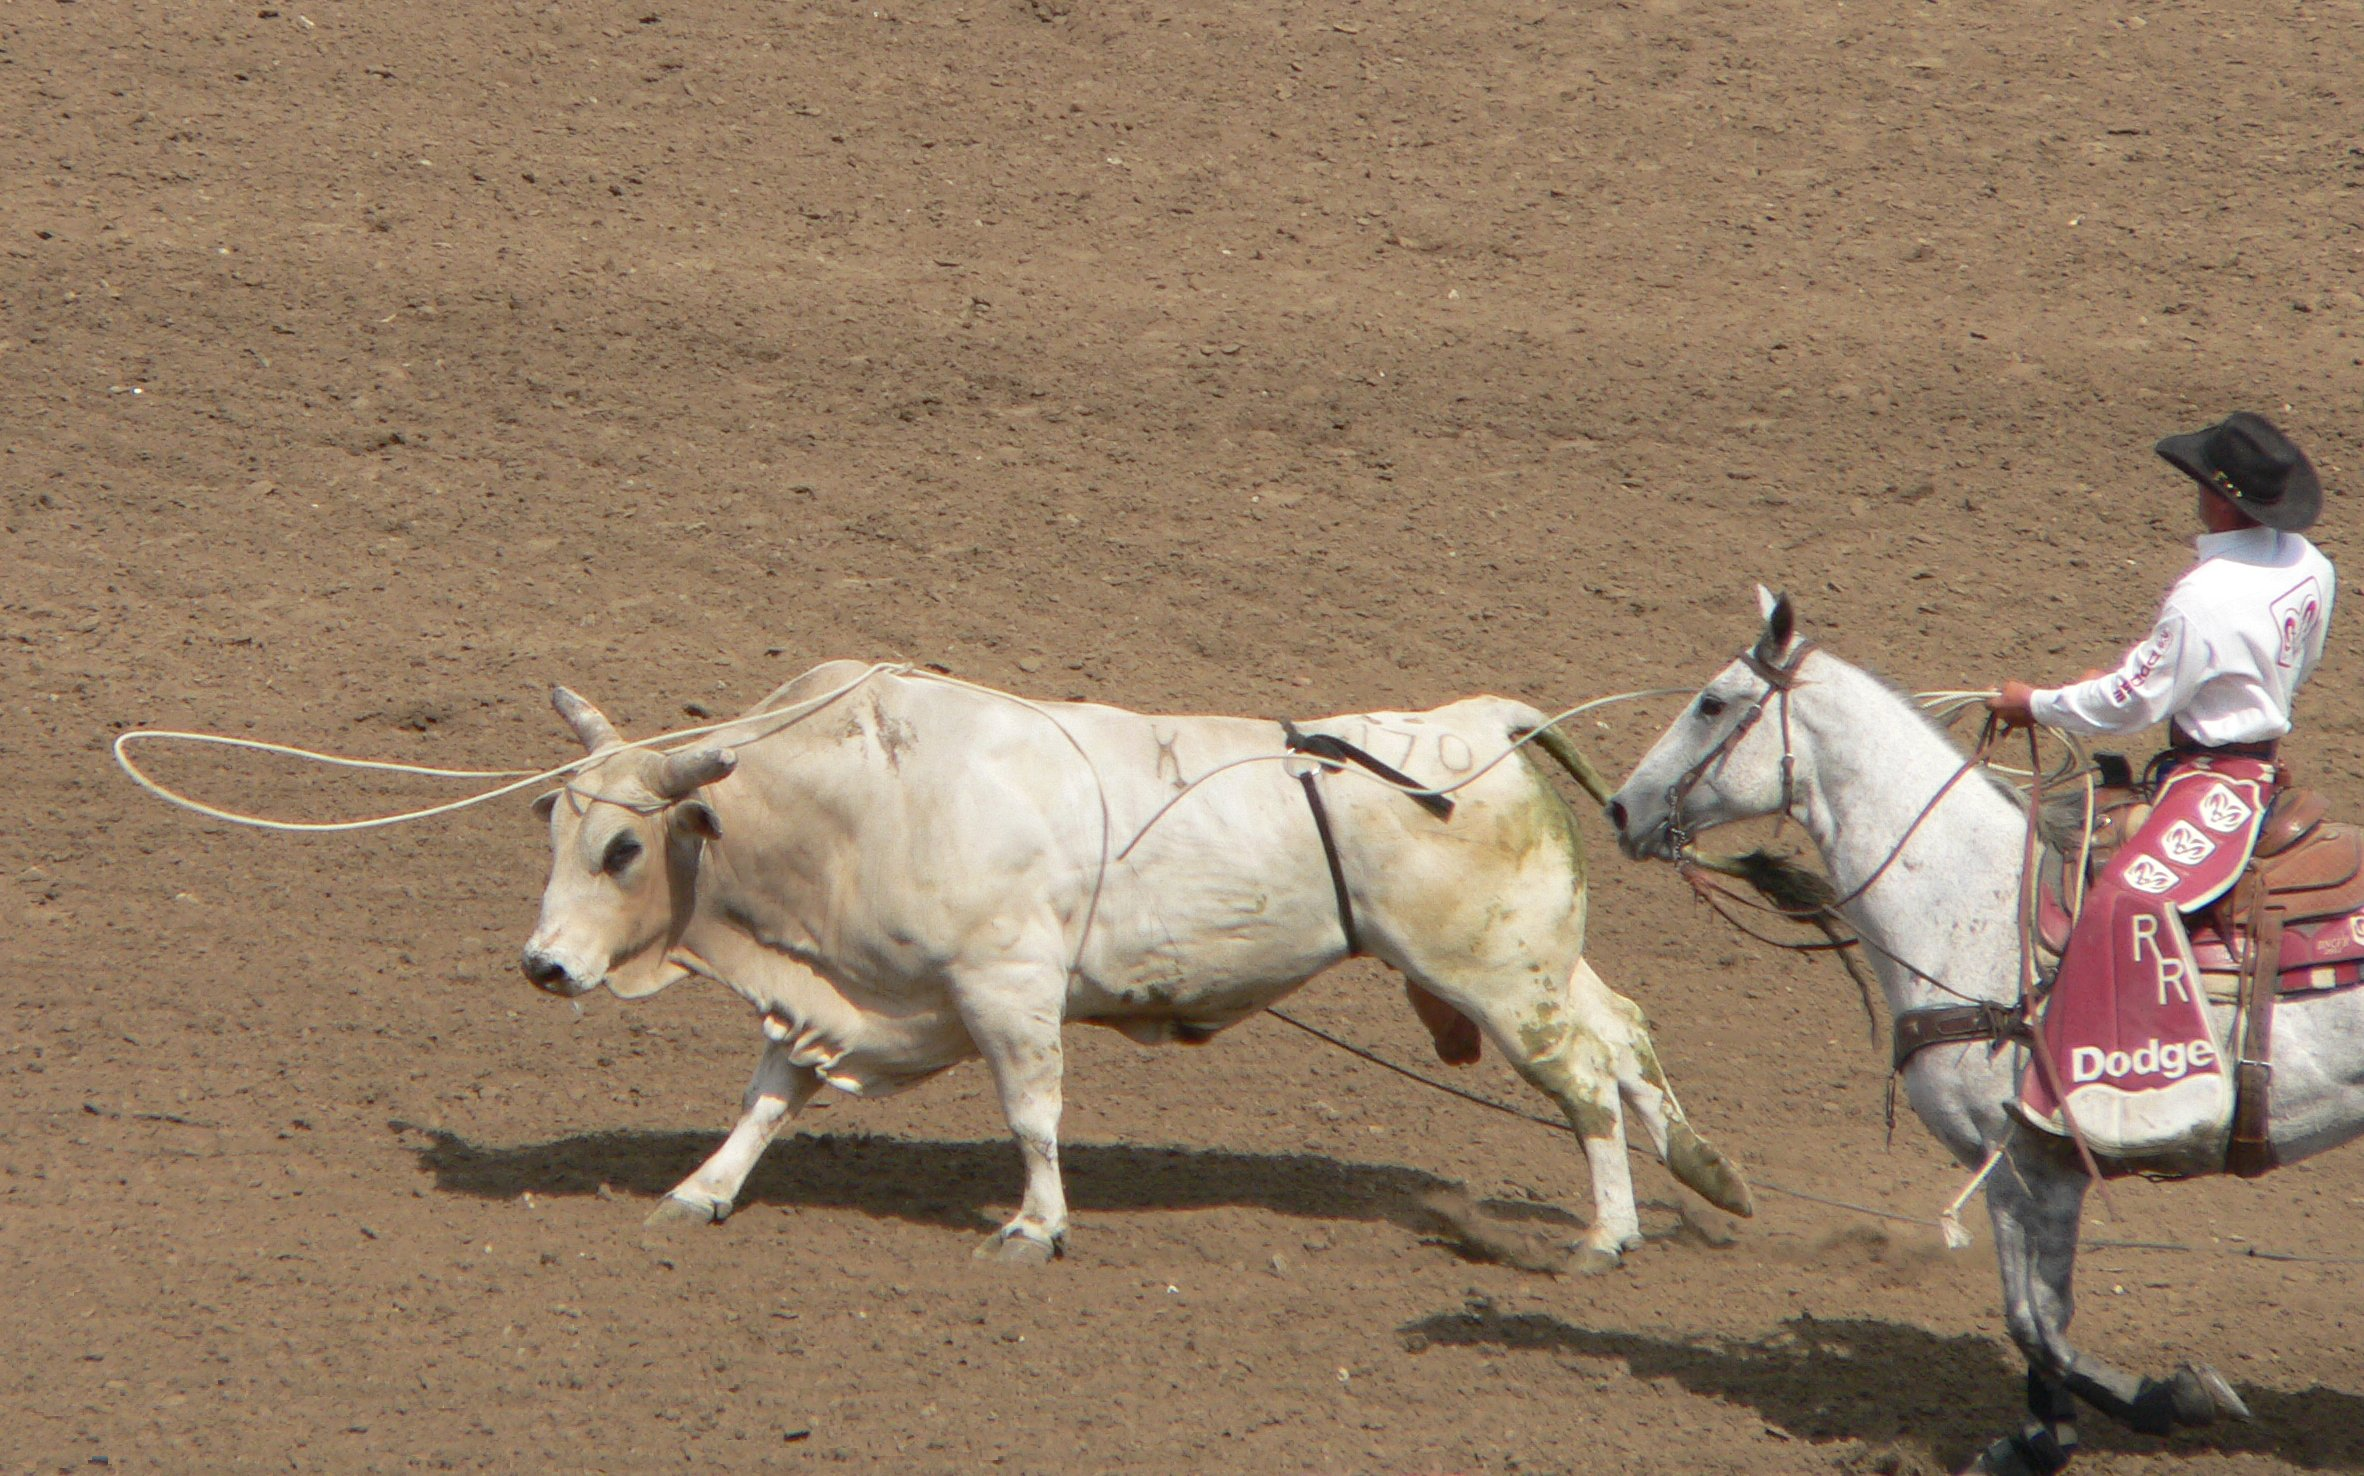
\includegraphics[width=0.7 \linewidth]{Figures/California_rodeo_Salinas_lasso_bull_p1050544.jpg}
    \caption{Traditional cowboy lasso.}
    \label{fig:11}
\end{figure}
\begin{figure}[htbp]
    \centering
    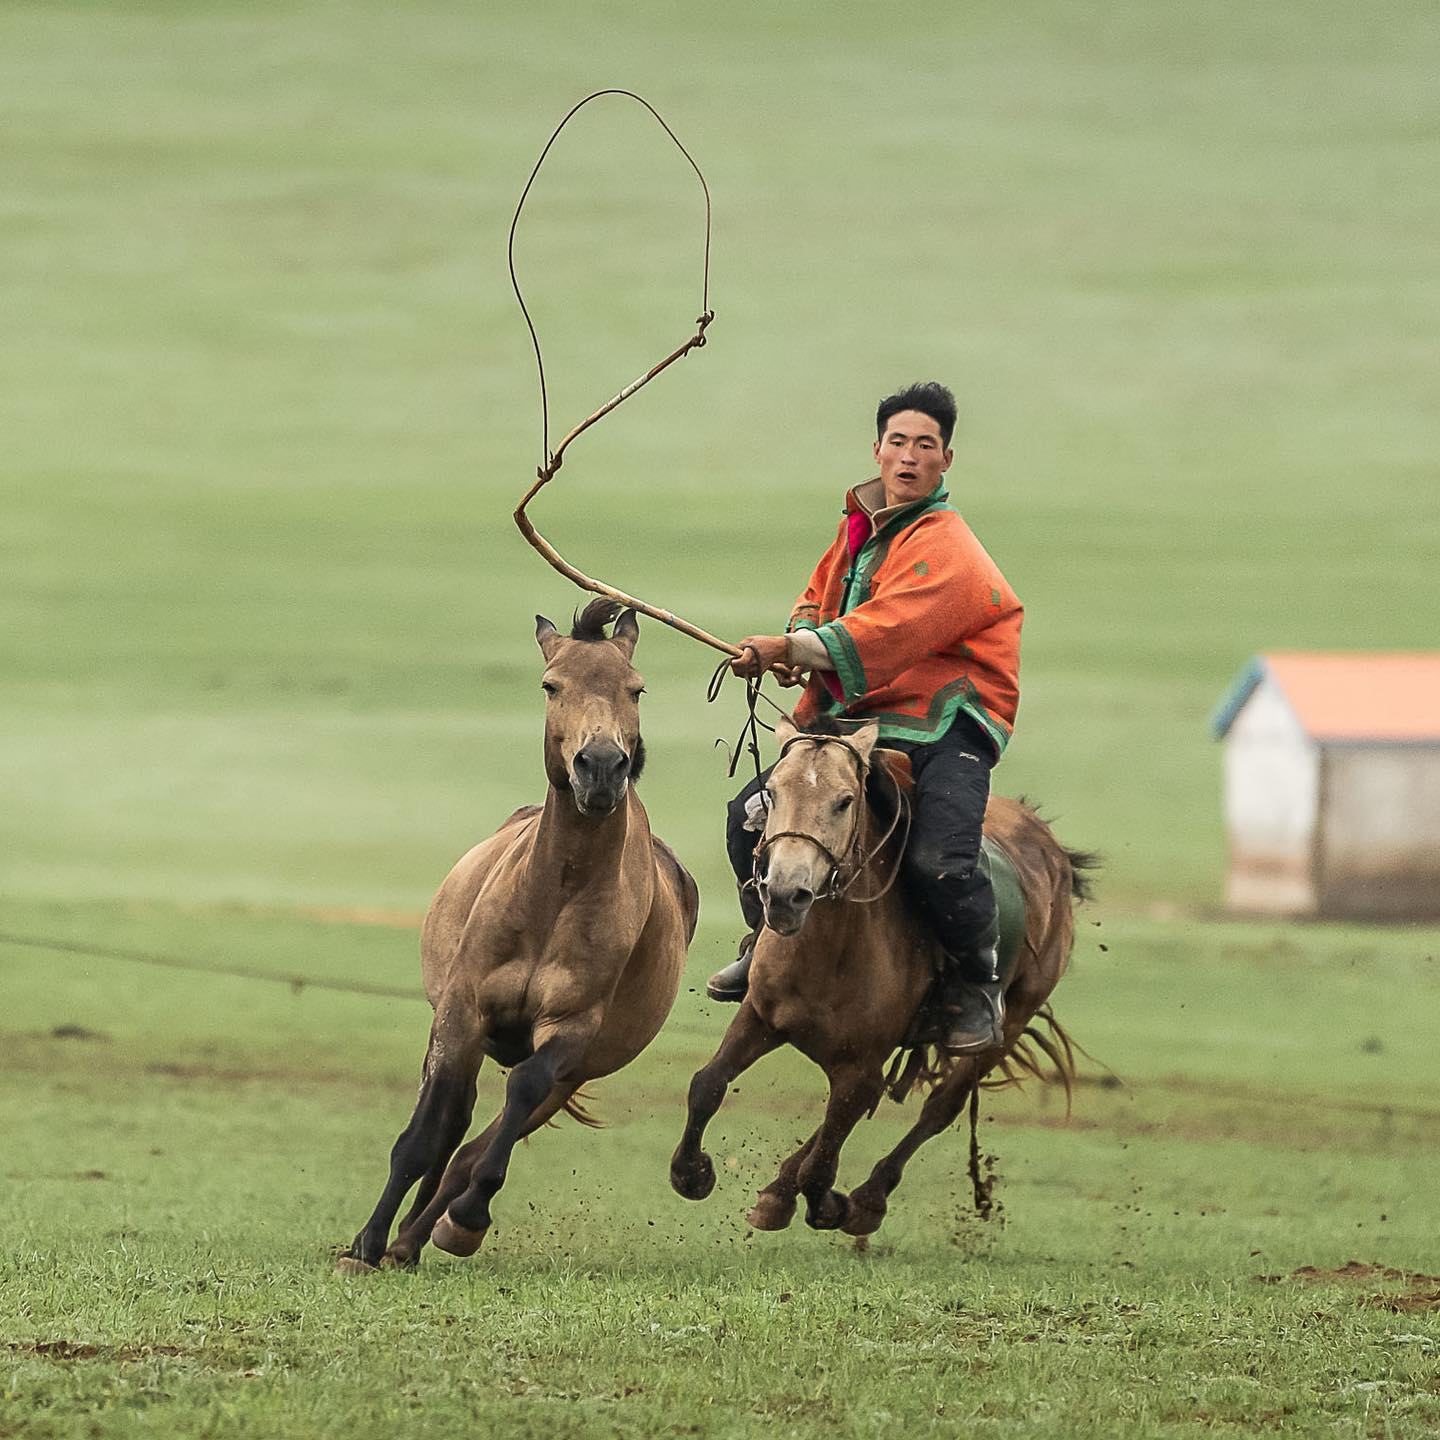
\includegraphics[width=0.7 \linewidth]{Figures/uurga.jpg}
    \caption{Traditional Mongolian uurga.}
    \label{fig:12}
\end{figure}

\begin{figure}[htbp]
\centering
\begin{tabular}{cc}
\begin{minipage}[t]{0.9\textwidth}
\centering
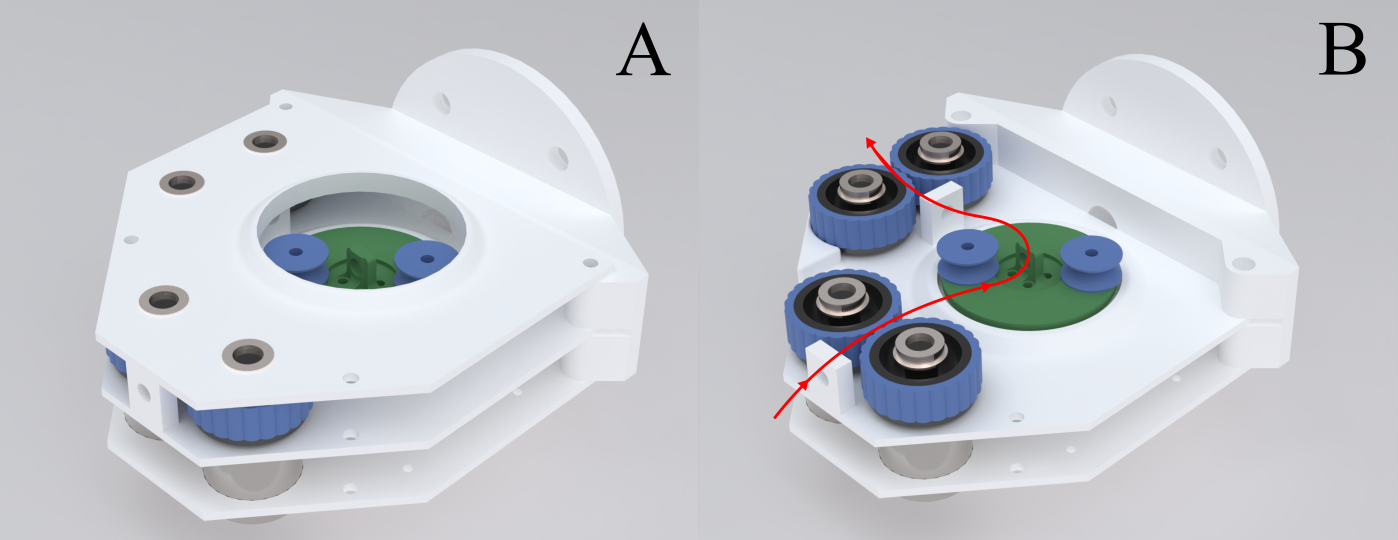
\includegraphics[width=\linewidth]{Figures/Figure1.png}
\caption{Prototype of Lasso Gripper.}
\label{fig:prototype_lasso_gripper}
\end{minipage}
\end{tabular}
\end{figure}

Within this thesis, Lasso Gripper serves as the main mechanism innovation and the central experimental platform. Its development makes it possible to study several mechanism-level questions: how tension can be maintained during reversible actuation, how launch-and-retraction dynamics affect capture range, how a flexible loop can improve robustness to object uncertainty, and how remote actuation can be coordinated to preserve low distal complexity. These questions define the main exploratory contribution of the thesis.

The handheld laparoscopic instrument examines the same tendon-driven variables in a much more constrained application domain. In laparoscopic surgery, surgeons manipulate long and slender tools through small incisions, which severely restrict distal dexterity and attenuate direct haptic perception, as illustrated in Fig.\ref{fig:13}. Conventional instruments typically provide only basic grasping and rotation, while more advanced articulated systems must balance dexterity against weight, complexity, and controllability. Tendon-driven actuation is highly relevant in this context because it permits motors to remain proximal while producing multiple distal degrees of freedom. However, the medical setting imposes additional constraints on size, ergonomic balance, repeatability, safety, and motion fidelity.
\begin{figure}[htbp]
    \centering
    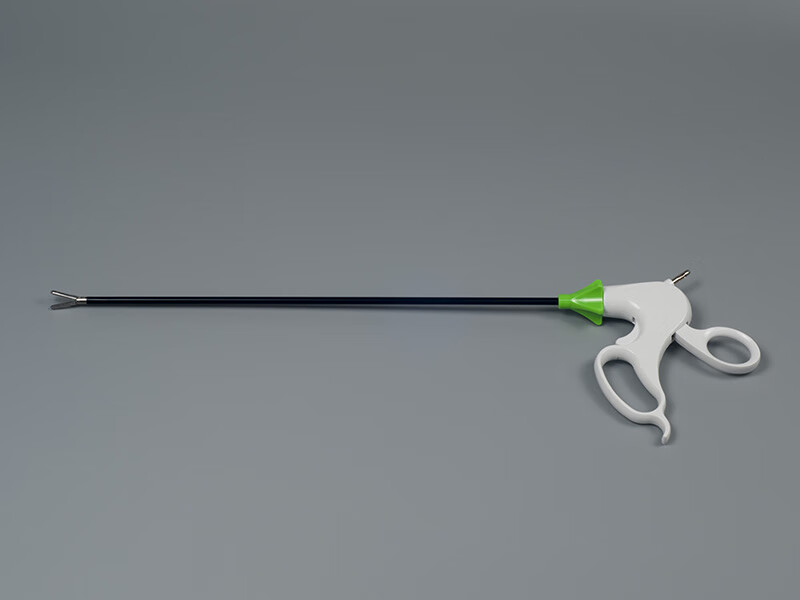
\includegraphics[width=0.7 \linewidth]{Figures/surgical instrument.jpg}
    \caption{Typical single-hole surgical instruments with limited distal dexterity.}
    \label{fig:13}
\end{figure}

The handheld laparoscopic instrument is therefore framed as a complementary application case within the same tendon-driven mechanism framework. It is not treated as a derivative of Lasso Gripper. Instead, it shows how related mechanism variables, including proximal actuation, differential tendon routing, explicit tension management, and sensor-supported control, can be organized in a compact handheld system under practical clinical constraints. This positioning keeps Lasso Gripper as the main innovative platform while allowing the thesis to examine tendon-driven design in a second, application-oriented setting.

The main contributions of this thesis are summarized as follows:
\begin{enumerate}
    \item A mechanism-level study of tendon-driven robotic systems focused on tension management, proximal actuation, compliant interaction, and low distal inertia.
    \item The design, fabrication, and experimental validation of Lasso Gripper as a novel tendon-driven mechanism for adaptive robotic grasping.
    \item The design and implementation of a handheld motorized laparoscopic instrument as a complementary application-oriented tendon-driven system for minimally invasive manipulation.
    \item A unified thesis narrative showing how tendon-driven mechanism principles can be organized across a primary adaptive grasping platform and a secondary medical-device application case.
\end{enumerate}

The remainder of this thesis is organized to follow that mechanism-centered narrative. Chapter 2 reviews related work in laparoscopic end-effectors and adaptive grasping systems, with emphasis on actuation, sensing, and tendon-driven design trade-offs. The subsequent chapters present Lasso Gripper as the primary contribution, including its mechanism design, grasping strategy, dynamic behavior, and experimental validation. The thesis then presents the handheld surgical instrument as a complementary application case under the same tendon-driven framework, focusing on compact device architecture, cable routing design, sensing strategy, and control implementation. The final chapters discuss the broader implications of these results and outline future directions for tendon-driven robotic mechanisms.

\let\cleardoublepage\clearpage

\chapter{Related Works}

\begin{chaptersummary}
This chapter surveys prior work relevant to adaptive and enveloping grasping as well as tendon-driven laparoscopic end-effectors. It covers loop- and belt-based grippers, sensorized soft grippers, material and microstructure innovations, grasp planning algorithms, actuation technologies, sensing strategies, tip and rod architectures, soft and continuum approaches, and AI-assisted monitoring and control.

The review highlights recurring challenges, including cable coupling, material creep and stretch, frictional losses, and the trade-offs between flexibility, load capacity, and sensing complexity. It identifies open gaps that motivate this thesis: compact, tension-preserving cable routing; miniature sensing for closed-loop compensation; mechanism-level evaluations linking design choices to performance; and robust sensing and routing strategies for loop-based grippers, which Lasso Gripper seeks to explore as the main mechanism platform.
\end{chaptersummary}

\section{Advances in Actuation Technologies for Multi-DOF End-Effectors in Laparoscopic Instruments}

Minimally Invasive Surgery (MIS) shifted instrument design toward restoring distal dexterity within severe access constraints. Cable-driven actuation is widely used because it enables multi-degree-of-freedom tips with low distal mass, but it brings challenges such as cable coupling, material creep, and reduced control fidelity. This section summarizes actuation alternatives, sensing strategies for tension and pose estimation, and tip/shaft design patterns that motivate the tendon-driven choices explored in this thesis.

To address the limited dexterity at the instrument tip, a prominent solution involves using cables as a medium to transmit power from the handpiece to the end-effector, thereby enabling additional DOFs, such as roll or yaw rotations. First introduced in the late 1990s, Intuitive Surgical's da Vinci system exemplifies this approach, employing a cable-driven mechanism to control its articulated tips. The primary advantage of such a system is that cables can transmit power over a distance with a lower weight penalty compared to rigid linkages or gear trains\cite{brodie_future_2018}. However, this benefit is accompanied by inherent challenges. In the initial design of the da Vinci system, cable coupling, where the movement of one cable inadvertently affects another, was a significant issue that could not be overlooked, often leading to kinematic inaccuracies and reduced control fidelity. Therefore, various approaches have been studied to address these problems.

\subsection{Replacements of Driven Motors}
\begin{figure}[htbp]
\centering
\begin{subfigure}[t]{0.48\textwidth}
\centering
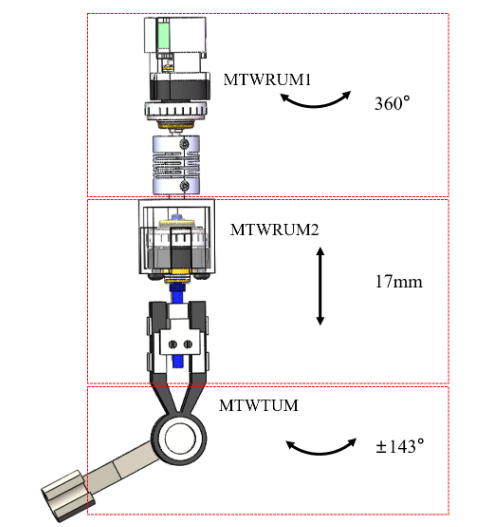
\includegraphics[width=\linewidth]{Figures/magnetic.png}
\caption{Design and illustration of ultrasonic motors\cite{li_design_2022}.}
\label{fig31a}
\end{subfigure}
\hfill
\begin{subfigure}[t]{0.48\textwidth}
\centering
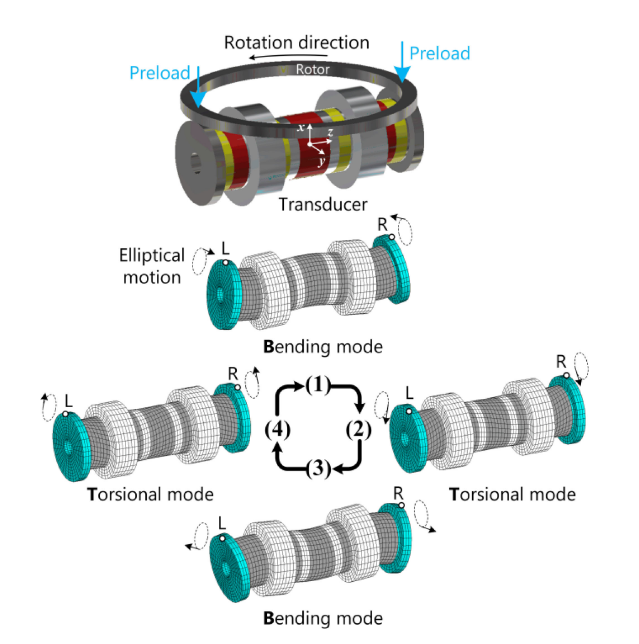
\includegraphics[width=\linewidth]{Figures/bending torsion.png}
\caption{Bending and torsion layouts of the transducer\cite{wu_rotary_2021}.}
\label{fig31b}
\end{subfigure}

\vspace{0.5em}

\begin{subfigure}[t]{0.48\textwidth}
\centering
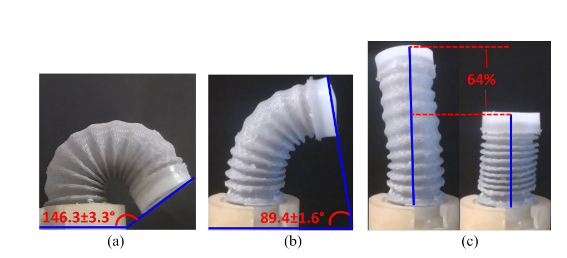
\includegraphics[width=\linewidth]{Figures/soft modular.png}
\caption{Flexible fluidic actuators with granular jamming for variable stiffness\cite{ranzani_soft_2016}.}
\label{fig31c}
\end{subfigure}
\hfill
\begin{subfigure}[t]{0.48\textwidth}
\centering
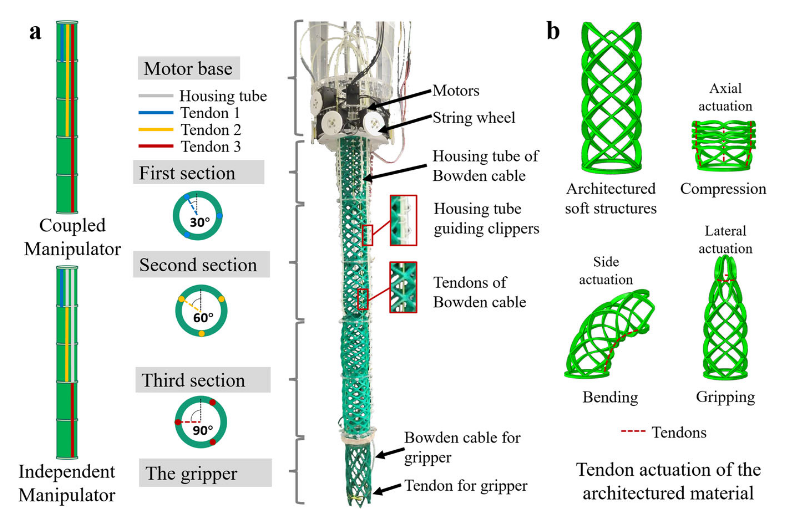
\includegraphics[width=\linewidth]{Figures/trimmed.png}
\caption{The tendon-driven manipulator design with trimmed helicoids\cite{guan_trimmed_2023}.}
\label{fig31d}
\end{subfigure}

\caption{Selected actuation and compliant tip technologies from recent MIS research. (a) ultrasonic motors; (b) bending and torsion transducer layouts; (c) flexible fluidic actuators with granular jamming for variable stiffness; (d) tendon-driven trimmed helicoid manipulator.}
\label{fig31}
\end{figure}

To address the challenges of control fidelity loss and restricted tip articulation in minimally invasive surgical instruments, various driving mechanisms have been extensively investigated. One prominent approach involves the implementation of ultrasonic motors as alternatives to conventional electromagnetic actuators. As illustrated in Fig. \ref{fig31a}, experimental validation has confirmed that the maximum output torque reaches $1.2\,\mathrm{mN\,m}$ for the rotary configuration and $1.4\,\mathrm{mN\,m}$ for the tilting mechanism. These torque values adequately satisfy the operational requirements of magnetically anchored laparoscopes while offering superior positional precision. Crucially, performance evaluations of the prototype system have substantiated both the feasibility and effectiveness of integrating these ultrasonic motors into laparoscopic applications\cite{kiong_tan_precision_2015}. This approach presents a novel and practical alternative for achieving enhanced visual platform maneuverability in single-port surgery, addressing fundamental limitations in conventional cable-driven systems through improved torque transmission and positioning accuracy.

Some studies focus on matching the power density and peak torque output of this proposed driving method to those of electromagnetic actuators. By applying a rod-shaped transducer in torsional and bending modes, the rotor is driven in its orthogonal direction with external excitations at specific frequencies. By adjusting the excitation frequencies, the maximum torque recorded in the experiments reached $10.1\,\mathrm{N\,m}$, and the output power reached $38.1\,\mathrm{W}$\cite{wu_rotary_2021}.

\subsection{Additional Sensors}

A fundamental limitation in the original cable-driven system involves the progressive uncertainty of cable length resulting from material creep during prolonged operation. This phenomenon introduces cumulative positioning errors between the input and output ends, significantly compromising control fidelity\cite{liang_novel_2017}. To mitigate this inherent uncertainty, the integration of supplemental sensing modalities has been implemented. These sensors enable real-time monitoring of either cable tension, end-effector pose, or both, facilitating a closed-loop control architecture that dynamically compensates for length variations and restores positional accuracy.



Accurate measurement of cable tension during surgical procedures represents a critical safety requirement in cable-driven robotic systems. In traditional laparoscopic surgery, surgeons rely on haptic feedback transmitted through rigid instruments to assess tissue interaction forces. However, in motor-driven systems where actuation forces are generated remotely, this crucial tactile information becomes significantly attenuated. This sensory disconnect necessitates extensive training for surgeons to develop appropriate motor control through the handheld interface, as demonstrated in studies on force sensing in robotic surgery \cite{trejos_force_2010}.

Force sensing has emerged as a promising solution to restore this lost feedback. The most straightforward approach involves embedding force sensors, such as Fiber Bragg Gratings (FBGs), directly into the surgical instrument. As explored in research on mechatronic design of force sensors\cite{zemiti_mechatronic_2007}, this method enables direct measurement of interaction forces at the end-effector. However, this integration often results in structural redundancy and increased instrument diameter, creating bulky designs that may compromise surgical access and maneuverability in confined operative fields.

To address these limitations, recent research has focused on miniaturized sensing strategies. One innovative approach involves embedding FBGs within precisely machined grooves on inclined cantilevers within the instrument structure\cite{xue_design_2018}. This design exploits the strain measurement capabilities of FBGs to detect minute deformations in the cantilevers caused by cable tension variations. The inclined configuration amplifies these deformations, enabling high-sensitivity force measurement while maintaining a compact form factor compatible with the dimensional constraints of minimally invasive instruments.

\subsection{Novel Structures of the Tip and Rod Design }

In conventional master-slave robotic systems, such as the da Vinci Surgical System and similar handheld robotic instruments, the end-effector typically provides 4 to 5 DOFs. This configuration is designed to replicate the articulation capabilities of the human wrist and fingers, enabling complex maneuvers like pitching, yawing, rolling, and grasping. However, a significant design limitation persists: these multiple DOFs are concentrated exclusively at the distal tip, while the connecting shaft or linkage primarily functions as a passive rotary base.

This recognition of ergonomic limitations in conventional articulated instruments has stimulated significant research into alternative tip architectures in recent years. With advances in the modeling and control of continuum robots, their design principles have been increasingly translated into the medical domain. Unlike traditional tip designs composed of multiple rigid links connected by discrete joints, continuum robots offer a validated scheme for implementing soft or continuously flexible connections, both between the tip and the instrument shaft, and among individual subcomponents of the tip itself. This paradigm shift enables a more distributed deformation along the instrument's length, effectively increasing the overall dexterity without concentrating all articulation at a single point. The resulting designs, often drawing inspiration from biological structures like tentacles or snakes, promise to mitigate surgeon fatigue by decoupling the end-effector's pose from the precise position of the surgeon's hand, thereby offering a more intuitive and ergonomic manipulation platform for complex surgical tasks.
Building upon the foundational research in continuum robotics, recent studies have explored innovative structural designs to enhance surgical instrument dexterity and safety. Ranzani et al. (2016) demonstrated a significant advancement by integrating flexible fluidic actuators within a silicone matrix containing multiple pneumatic chambers. This design enabled multidirectional bending and elongation capabilities. The proposed manipulator employed a modular architecture, utilizing granular jamming techniques to achieve dynamic stiffness variation and diverse movement profiles, as illustrated in Fig.~\ref{fig31c}.
Further extending this paradigm, researchers have investigated the transition from rigid linkages to compliant structures to substantially improve operational flexibility. One notable approach involves manipulating the trimmed angle of a helicoid structure to create a variable-stiffness robotic arm\cite{guan_trimmed_2023}. When coupled with a cable-driven actuation system, this design achieves an expanded workspace while significantly minimizing the risk of iatrogenic tissue damage during surgical procedures, as shown in Fig.~\ref{fig31d}. These developments in soft robotics and variable-stiffness mechanisms represent promising directions for next-generation surgical instruments that balance precision with patient safety.

\subsection{AI-Assisted Monitoring and Control}
As analyzed in previous sections, contemporary research in medical instrumentation predominantly advances along three interconnected fronts: innovative tip design, integrated sensory feedback systems, and intelligent control algorithms. The rapid evolution of Deep Learning and Reinforcement Learning methodologies has now catalyzed a fourth research direction: the integration of data-driven approaches into clinical practice.

A particularly promising development lies in repurposing the existing endoscopic camera, initially intended solely for surgical visualization, as an external verification system for instrument navigation. Specifically, Kong et al. (2023) demonstrated that through a specially designed architecture, both the visual stream from the camera and kinematic data from the actuation motors can be fused to estimate the positional discrepancy between commanded and actual end-effector positions following movement execution\cite{kong_automatic_2023}. This estimated deviation is subsequently converted into compensation signals that drive automatic self-correction maneuvers, effectively creating a vision-enhanced closed-loop control system that continuously calibrates the instrument without requiring additional hardware beyond the standard surgical setup.

This methodology represents a significant paradigm shift from traditional model-dependent control strategies, leveraging the wealth of available surgical video data to address inherent system limitations such as cable stretch, hysteresis, and kinematic modeling inaccuracies. The approach demonstrates how computer vision and deep learning techniques can transform existing surgical infrastructure into a self-calibrating system, potentially enhancing both positioning accuracy and long-term reliability in cable-driven surgical instruments.

\subsection{Synthesis of Design Gaps for Handheld Tendon-Driven Instruments}

The reviewed literature shows that no single design direction fully resolves the practical requirements of a handheld multi-DOF surgical instrument. Distal motors and ultrasonic actuators can improve local responsiveness, but they tend to increase distal complexity and may create packaging or thermal-management concerns. Cable-driven and tendon-driven architectures relocate actuation proximally and therefore reduce distal mass, but introduce nonlinear transmission effects such as coupling, backlash, friction, and hysteresis. Continuum and soft structures improve access and safety, yet their compliance can make precise tip positioning and high-load manipulation more difficult without additional sensing or compensation.

These trade-offs motivate the design strategy adopted in this thesis. Rather than treating actuation, sensing, routing, and control as separate subproblems, the proposed handheld instrument is organized around explicit tension management. The mechanical layout preserves proximal actuation, paired cable routing, and quick-swap modularity; the input stage separates user-intent sensing from distal actuation; and the control implementation uses low-level servo feedback to constrain cable motion. Table~\ref{tab:surgical_lit_synthesis} summarizes the main design implications extracted from the related work and maps them to the design decisions used later in the thesis.

\begin{table}[htbp]
    \centering
    \caption{Synthesis of surgical-instrument literature and implications for this thesis}
    \label{tab:surgical_lit_synthesis}
    \begin{tabular}{p{0.23\linewidth} p{0.25\linewidth} p{0.24\linewidth} p{0.18\linewidth}}
        \toprule
        Research direction & Main advantage & Remaining limitation & Thesis response \\
        \midrule
        Distal or miniature actuation & Direct local actuation and high responsiveness & Added distal mass, packaging difficulty, and possible heat or wiring burden & Keep heavier actuation proximal and transmit motion through cables \\
        Cable/tendon transmission & Low distal inertia and compact multi-DOF motion & Coupling, backlash, friction, cable stretch, and hysteresis & Use paired winding, guided routing, and feedback-supported tension management \\
        Embedded force or shape sensing & Improved safety and closed-loop compensation & Increased structural complexity and integration burden & Use compact input sensing and servo-state feedback in the current prototype \\
        Soft and continuum mechanisms & Compliance, safety, and large bending range & Reduced stiffness and harder high-precision control & Retain rigid load-bearing tip while using cable compliance for safer interaction \\
        Vision and learning-based compensation & Potential correction of unmodeled errors & Requires training data, validation, and robust perception & Reserved as a future calibration and adaptive-control pathway \\
        \bottomrule
    \end{tabular}
\end{table}

This synthesis also clarifies the relationship between the surgical instrument and Lasso Gripper. Both systems rely on flexible tensile elements to transmit motion and regulate interaction forces, but they emphasize different operating regimes and play different roles in the thesis. Lasso Gripper is the primary mechanism contribution and uses a free loop to maximize capture tolerance in open manipulation. The surgical instrument is a complementary application case that constrains the cable path through guide tubes, pulleys, and reels to maximize repeatability in a compact handheld device. The literature review therefore motivates a common mechanism question for the remainder of the thesis: how can flexible tensile transmission be designed so that its compliance is useful rather than a source of uncontrolled error?

%%%%%%%%%%%%%%%%%%%% Chapter 2
%\chapter{Related works} % Main chapter title
%\label{Chapter2} % For referencing the chapter elsewhere, use 
%----------------------------------------------------------------------------------------
\section*{Chapter summary}
\noindent
This chapter reviews developments in adaptive and enveloping grasping, with emphasis on loop- and belt-based grippers, sensorized soft grippers, material and microstructure innovations, and grasp planning algorithms. The survey synthesizes how these approaches trade off shape adaptability, load capacity, and sensing complexity.

\noindent
The literature suggests that loop-based grippers offer strong advantages in distributed contact and tolerance to positional uncertainty, but they require robust sensing and routing strategies to handle dynamic targets and scale to diverse applications — issues the Lasso Gripper prototype seeks to explore.

\section{Development of Adaptive Grasping and its application}
\subsection{The Necessity of Enveloping and Encircling Grasping}
Enveloping and encircling grasping provide enhanced stability and shape adaptability for a wide range of objects. This subsection reviews recent structural and control approaches that achieve enveloping grasps and highlights the remaining limitations that motivate loop-based and tendon-driven solutions.

One notable study introduces a dual-mode soft robotic gripper designed with integrated  annular structures and a contraction actuator. This design significantly improves shape tolerance and gripping force by altering the contact method between the gripper and the object, adjusting the stiffness and load capacity through controlled material properties \cite{hu2023dual}.

Another novel technique employs a soft gripper that leverages a belt loop with an actuated adhesion mechanism. This mechanism provides dual-directional force – both radial and tangential – which enhances the effectiveness and stability of the grasping action. The minimal interaction force strategy ensures gentle handling, making it suitable for fragile objects \cite{chen2024soft}.

Additional studies introduce an affordable, underactuated compliant gripper capable of adapting to objects of diverse sizes and shapes. The design features a flexure motion transmission mechanism and multifunctional jaws, allowing for a more conforming grasp. This interaction between the gripper and the target object increases both gripping force and stability \cite{sun2024low}.

Additionally, a study on a tendon-driven robotic gripper highlights the importance of stable enveloping grasps. By optimizing tendon routes and stiffness, this gripper can perform multiple grasping modes, including parallel, enveloping, and fingertip grasps. This versatility ensures the gripper's flexibility and stability across various applications \cite{ciocarlie2014velo}.

Enveloping and encircling grasping techniques are crucial in robotic grasping technology. They enhance shape adaptability, gripping force, and stability, providing robust support for robots in complex and dynamic environments.
\begin{figure}[htbp]
\centering
\begin{tabular}{cc}
\begin{minipage}[t]{0.5\textwidth}
\centering
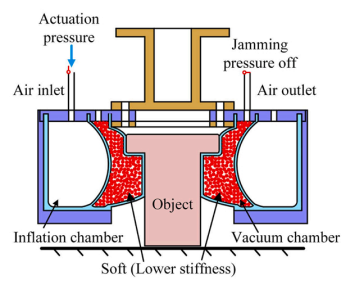
\includegraphics[width=0.7\columnwidth]{Figures/1.png}
\caption{Pressurized the actuation chamber and adaptive grasping \cite{hu2023dual}}
\end{minipage}
\qquad
\begin{minipage}[t]{0.5\textwidth}
\centering
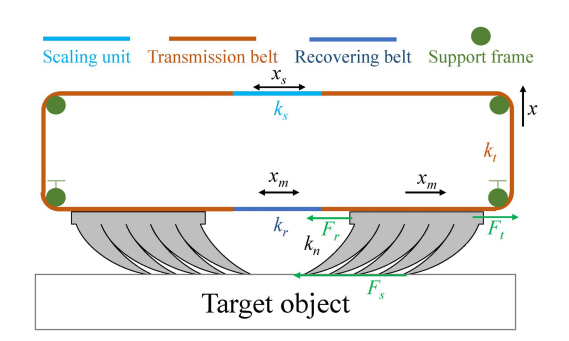
\includegraphics[width=0.7\columnwidth]{Figures/8.png}
\caption{Belt Loop Actuated Adhesion Design \cite{chen2024soft}}
\end{minipage}
\end{tabular}
\begin{tabular}{cc}
\begin{minipage}[t]{0.5\textwidth}
\centering
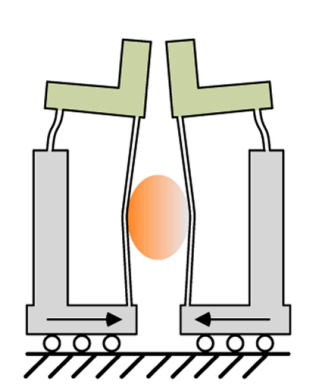
\includegraphics[width=0.7\columnwidth]{Figures/4.png}
\caption{Enveloping grasps of the multifunctional jaw \cite{sun2024low}}
\end{minipage}
\qquad
\begin{minipage}[t]{0.5\textwidth}
\centering
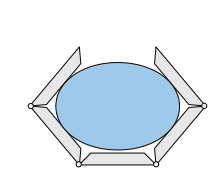
\includegraphics[width=0.7\columnwidth]{Figures/172.png}
\caption{Examples of enveloping grasps of Velo gripper \cite{ciocarlie2014velo}}
\end{minipage}
\end{tabular}
\end{figure}





\subsection{Grasping System with Integrated Sensors}

The integration of sensors with soft materials such as loops significantly enhances the efficiency and adaptability of robotic grasping systems. Various studies have demonstrated the potential benefits of combining these elements to improve performance in different contexts.

A notable example is a modular flying gripper that utilizes a loop gripper mechanism to control its position and pose flexibly. This system, composed of quadrotor-based modules, showcases the versatility of encircling grasping techniques. The decentralized control approach enables the flying gripper to modify its aperture angle, thereby facilitating efficient object grasping and transportation \cite{gabrich2018flying}.

In another study, a soft robotic gripper equipped with a liquid-metal sensing skin provides a robust feedback mechanism. This gripper, integrated with proximity, pressure, and orientation sensors, operates using shape-memory alloy springs to transition between open and close states. The closed-loop control enabled by these sensors allows the system to detect and respond to external disturbances, enhancing its grasping, release, and transportation capabilities \cite{yin2020closing}.

Further advancements are seen in the development of a continuum body gripper that incorporates flexible latex bladder sensors. By measuring air pressure changes, these sensors provide tactile and proprioceptive feedback, essential for delicate and high-force grasping. This integration allows the gripper to manage a diverse array of objects, ranging from heavy to fragile items, with minimal control input. The sensorized gripper demonstrates high sensitivity and repeatability, making it a cost-effective and durable solution for universal grasping applications \cite{hughes2020sensorization}.

Additionally, a visual-tactile fusion framework has been proposed to address the challenges of grasping transparent objects in complex environments. This framework combines visual and tactile data to enhance grasping efficiency. A tactile calibration technique combined with a visual-tactile fusion classification method greatly enhances the success rate and accuracy of grasping transparent objects. The experimental results validate the effectiveness of integrating tactile sensors within the gripper system, particularly for objects that are irregular or visually undetectable \cite{li2023visual}.

The combination of sensors with soft materials such as loops in robotic grippers offers significant improvements in grasping systems. These integrations provide enhanced feedback, adaptability, and control, rendering them invaluable for a wide array of applications, from delicate object handling to complex environmental interactions.

\begin{figure}[htbp]
\centering
\begin{tabular}{cc}
\begin{minipage}[t]{0.5\textwidth}
\centering
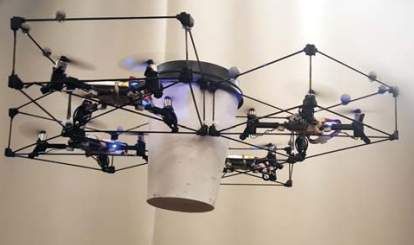
\includegraphics[width=0.7\columnwidth]{Figures/2.png}
\caption{The Flying Gripper holding a coffee cup \cite{gabrich2018flying}}
\end{minipage}
\qquad
\begin{minipage}[t]{0.5\textwidth}
\centering
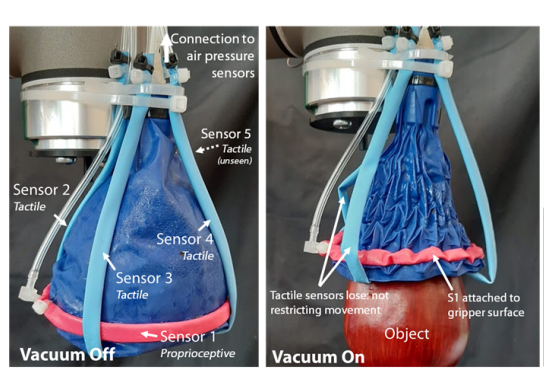
\includegraphics[width=0.7\columnwidth]{Figures/15.png}
\caption{The illustration of tactile sensor and pressure sensors integrated in the loop gripper \cite{hughes2020sensorization}}
\end{minipage}
\end{tabular}
\end{figure}



\subsection{Designing for the Physical Properties of Soft Gripper}

Through advancements in material technology and microstructural design, significant progress has been made in altering the physical properties of flexible materials like ropes. These innovations have paved the way for the development of more efficient and adaptable soft robotic grippers.

A groundbreaking soft gripper utilizing a self-sensing super-coiled polymer (SCP) actuator is introduced by Wang et al. (2021). This actuator is crafted from multi-strand sewing thread that undergoes a self-coiling process, enabling it to untwist when heated. The addition of a metal wire wrapped around the SCP enhances temperature measurement precision, forming a closed-loop control system for accurate gripper manipulation. This approach offers a foundation for customizing the physical properties of rope-like materials for actuator applications \cite{wang2021lightweight}.

Sun et al. (2020) described a soft gripper with adjustable stiffness, inspired by the behavior of pangolin scales. The gripper is composed of two layers: a variable stiffness layer and a pneumatic-driven layer. The variable stiffness layer emulates pangolin scales, remaining flexible during normal activities but becoming rigid when threatened. The toothed pneumatic actuator increases the gripper's stiffness, enabling it to grasp a wide range of objects effectively. The autonomous control system of this gripper collects feedback signals to adjust the stiffness autonomously, making it suitable for unstructured environments \cite{sun2020soft}.

Zhang et al. (2017) tackled the design problem of soft robots using a topology optimization framework. A pneumatically actuated soft gripper was developed, with three fingers each designed as a continuum compliant mechanism to achieve maximum bending deformation. This actuator was fabricated through 3D printing, and experimental results demonstrated its ability to grasp objects effectively. This optimization approach provides valuable insights for further exploration of the microstructure of lasso grippers \cite{zhang2017design}.

Li et al. proposed a soft gripper inspired by the inchworm's true leg. This design includes two rows of sharp hooks on a soft palm, with connections made via Shape Memory Alloy (SMA) springs. The design allows the gripper to adhere to rough surfaces and grasp objects with varying shapes and dimensions. The combination of elastic muscle-like structures and sharp hooks enhances the load-carrying capacity of the gripper, demonstrating the potential of microstructural design in soft robotics \cite{li2017development}.

Wang et al. (2017) explored the usage of Shape Memory Alloy (SMA) in soft grippers, addressing the inherent softness and low actuation force of traditional systems. The study described a soft gripper with variable stiffness based on SMA, composed of three fingers, each with two hinges. The hinges can achieve a significant change in stiffness, allowing the gripper to adapt to various shapes and weights. This material modification approach shows promise for effective grasping applications \cite{wang2017shape}.

The integration of advanced material technologies and microstructural designs has significantly enhanced the capabilities of soft robotic grippers. These innovations provide a robust foundation for developing adaptable and efficient grasping systems.

\begin{figure}[htbp]
\centering
\begin{tabular}{cc}
\begin{minipage}[t]{1\textwidth}
\centering
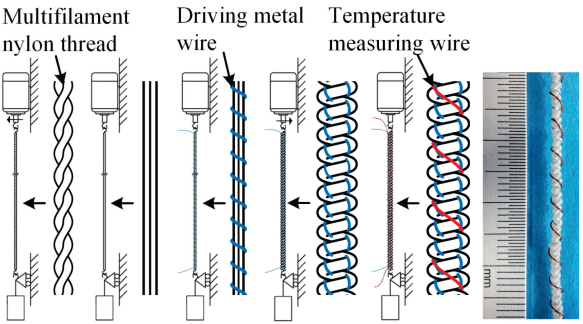
\includegraphics[width=0.7\columnwidth]{Figures/3.png}
\caption{Manufacturing process of actuator with multifilament nylon thread \cite{wang2021lightweight}}
\end{minipage}

\end{tabular}
\begin{tabular}{cc}
\begin{minipage}[t]{0.5\textwidth}
\centering
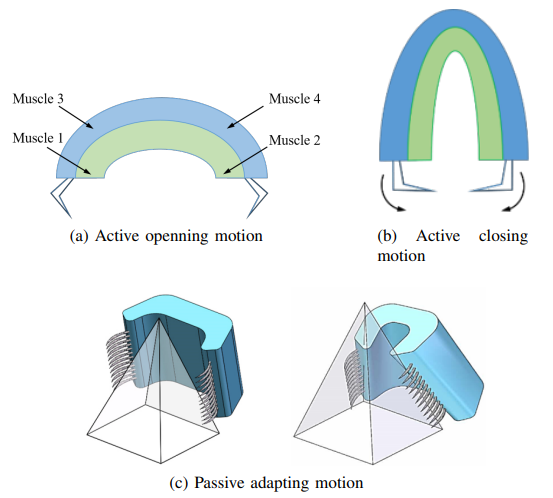
\includegraphics[width=0.7\columnwidth]{Figures/12.png}
\caption{Bio-mechanism of inchworm’s true leg \cite{li2017development}}
\end{minipage}
\qquad
\begin{minipage}[t]{0.5\textwidth}
\centering
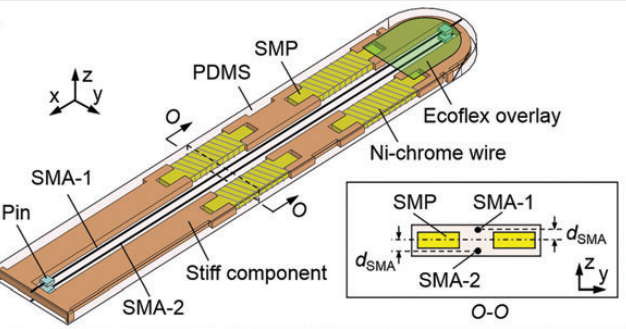
\includegraphics[width=0.7\columnwidth]{Figures/19.png}
\caption{Shape Memory Alloy-Based Soft Gripper \cite{wang2017shape}}
\end{minipage}
\end{tabular}
\end{figure}


\subsection{Advancement of Grasp Planning Algorithm for Lasso Grippers}

The design of grasping algorithms has made significant strides in enhancing the adaptability and efficiency of robotic grippers, particularly those employing rope-like structures such as lasso grippers. These algorithms leverage unique approaches to optimize grasp planning and ensure stable and robust manipulation.

Li et al. (2015) proposed an innovative grasp planning method that addresses the computational challenge of determining stable force-closure grasp configurations for multi-fingered hands. A low-level shape exploration technique is employed in this method by wrapping multiple cords around an object to quickly identify promising grasping regions. Using a variant of the close-until-contact procedure, contact points are determined by the algorithm, which then utilizes finger kinematics and contact information to filter out unstable grasps. This approach not only enhances the natural appearance of grasps but also improves efficiency, as it bypasses extensive preprocessing steps like segmentation and medial axis extraction. The adaptability of this method suggests that the structural concept of wrapping cords around objects can be effectively applied to lasso grippers, potentially offering superior grasping performance \cite{li2015fast}.

Fang et al. (2023) introduced the AnyGrasp algorithm, designed to enhance robust and efficient grasp perception across both spatial and temporal domains. This algorithm utilizes a dense supervision strategy, integrating real perception data with analytic labels to create a comprehensive training dataset. By incorporating object center-of-mass awareness into the learning process, AnyGrasp improves grasp stability. Additionally, it employs grasp correspondence across observations, enabling dynamic tracking of grasp poses, which ensures effectiveness even in noisy environments. The success of AnyGrasp in achieving a high success rate in bin clearing tasks underscores its potential applicability to various robotic grippers, including those with lasso structures \cite{fang2023anygrasp}.

These advancements in grasping algorithm design underscore the importance of innovative computational methods in enhancing the functionality of robotic grippers. The adaptive planning optimization demonstrated by Li et al. (2015) highlights the potential of rope-like structures in improving grasp performance. As the field continues to evolve, integrating these approaches with lasso grippers could lead to more versatile and effective robotic grasping systems.

\begin{figure}[htbp]
\centering
\begin{tabular}{cc}
\begin{minipage}[t]{0.6\textwidth}
\centering
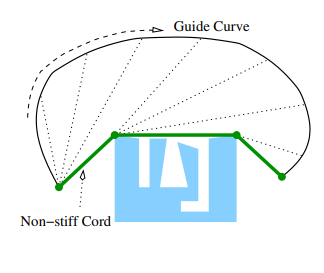
\includegraphics[width=0.7\columnwidth]{Figures/14.png}
\caption{Geometric construction of a non-stiff cord \cite{li2015fast}}
\end{minipage}

\end{tabular}

\end{figure}

\subsection{Application of Lasso Grippers in Real-World Scenarios}

The application of lasso grippers in various real-world scenarios demonstrates their versatility and effectiveness in handling a variety of objects with minimal control effort and high reliability. This section reviews recent advancements and practical implementations of lasso grippers across different fields.

Manes et al. (2024) introduced a soft cable loop-based gripper designed for robotic automation in chemistry laboratories. This gripper can reliably grasp cylindrical and prismatic objects of various sizes with minimal clearance. The design utilizes the compliance of a cable to completely envelop target objects, with support provided by a rigid finger once the grip is secured. This mechanism requires minimal control effort, making it highly practical for repetitive tasks in automated chemistry processes. The gripper demonstrated a grasp reliability with a failure rate of less than 1\%, showcasing its efficacy in handling delicate laboratory glassware. However, the use of a self-supporting plastic polymer material limits the loop size, as larger loops would fail to maintain their shape \cite{manes2024soft}.

\begin{figure}[htbp]
\centering
\begin{tabular}{cc}
\begin{minipage}[t]{1\textwidth}
\centering
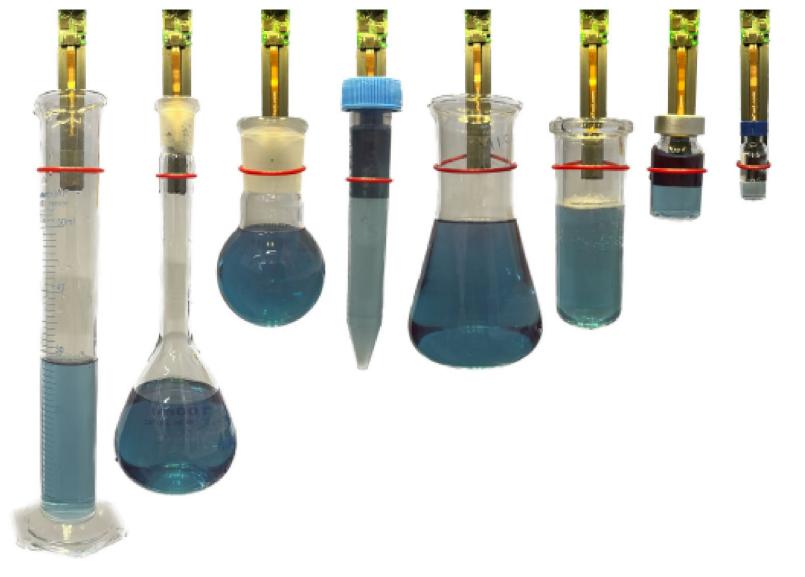
\includegraphics[width=0.7\columnwidth]{Figures/6.png}
\caption{A cable loop gripper prototype was evaluated for its ability to grasp various types of chemistry glassware. \cite{manes2024soft}}
\end{minipage}

\end{tabular}
\begin{tabular}{cc}
\begin{minipage}[t]{0.5\textwidth}
\centering
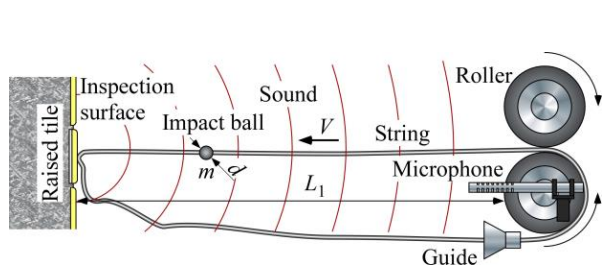
\includegraphics[width=0.7\columnwidth]{Figures/13.png}
\caption{String shoot impact towards a wall \cite{Japan2023}}
\end{minipage}
\qquad
\begin{minipage}[t]{0.5\textwidth}
\centering
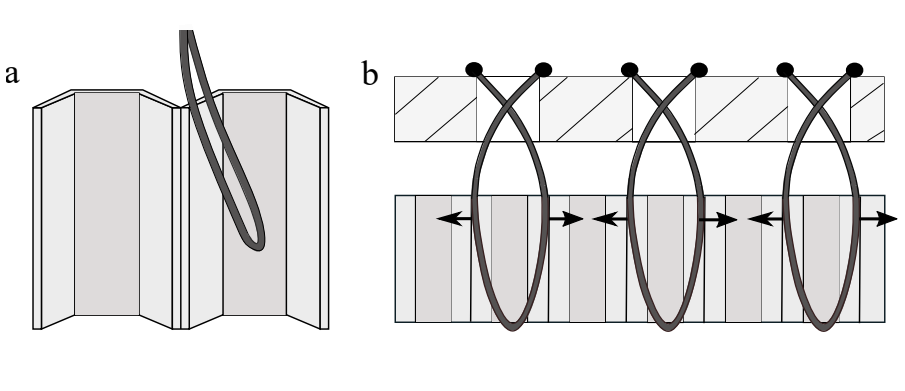
\includegraphics[width=0.7\columnwidth]{Figures/16.png}
\caption{String loop gripper for honeycomb materials \cite{roth2021loop}}
\end{minipage}
\end{tabular}
\end{figure}


A cable-driven gripper with perception capabilities for autonomous strawberry picking was developed by Xiong et al. (2018). The gripper utilizes six fingers to create a closed space around a target strawberry, gently cutting the stem without causing damage to the fruit. Equipped with infrared sensors, positional errors can be corrected by the gripper, enhancing robustness and achieving a high success rate in picking isolated strawberries. The integration of internal perception allows the gripper to tolerate positional inaccuracies, reducing the need for slow, high-level closed-loop control. This design highlights the advantages of using cable actuators, such as flexibility and biological friendliness, making it suitable for delicate agricultural applications \cite{xiong2018design}.

Roth et al. (2021) presented the Loop Gripper designed for handling honeycomb materials used in various industries. This gripper uses adjustable threads to provide the necessary flexibility and sensitivity to grip honeycomb panels without damaging their fragile cell walls. Through a series of tests, the optimal gripping parameters for various honeycomb materials were determined, proving the concept's suitability for automated gripping tasks. The Loop Gripper's approach of using a soft, structure-friendly force to grasp objects aligns with the principles of lasso grippers, emphasizing the importance of adaptability and gentle handling \cite{roth2021loop}.

These studies underscore the practical applications of lasso grippers in diverse fields, from chemistry laboratories to agricultural and material handling tasks. The inherent adaptability and gentle handling capabilities of lasso grippers make them an effective solution for various automated processes, demonstrating their potential for widespread adoption in real-world scenarios.




\subsection{The Balance between Flexibility and Strength}

Current research in robotic gripping mechanisms often focuses on achieving a balance between flexibility and strength. Pneumatic flexible grippers, for instance, offer excellent shape adaptability but are limited in their working range and load capacity. Yu et al. have noted that soft pneumatic actuators are widely utilized in soft robots, where their bending angles and motion rules at different pressures are crucial for practical applications \cite{yu2022modeling}. However, despite their flexibility, these actuators struggle with heavier loads and larger workspaces. Moreover, their dependency on precise pressure control can make them susceptible to performance inconsistencies, particularly in environments where maintaining stable pressure is challenging.

\begin{figure}[htbp]
\centering
\begin{tabular}{cc}
\begin{minipage}[t]{0.9\textwidth}
\centering
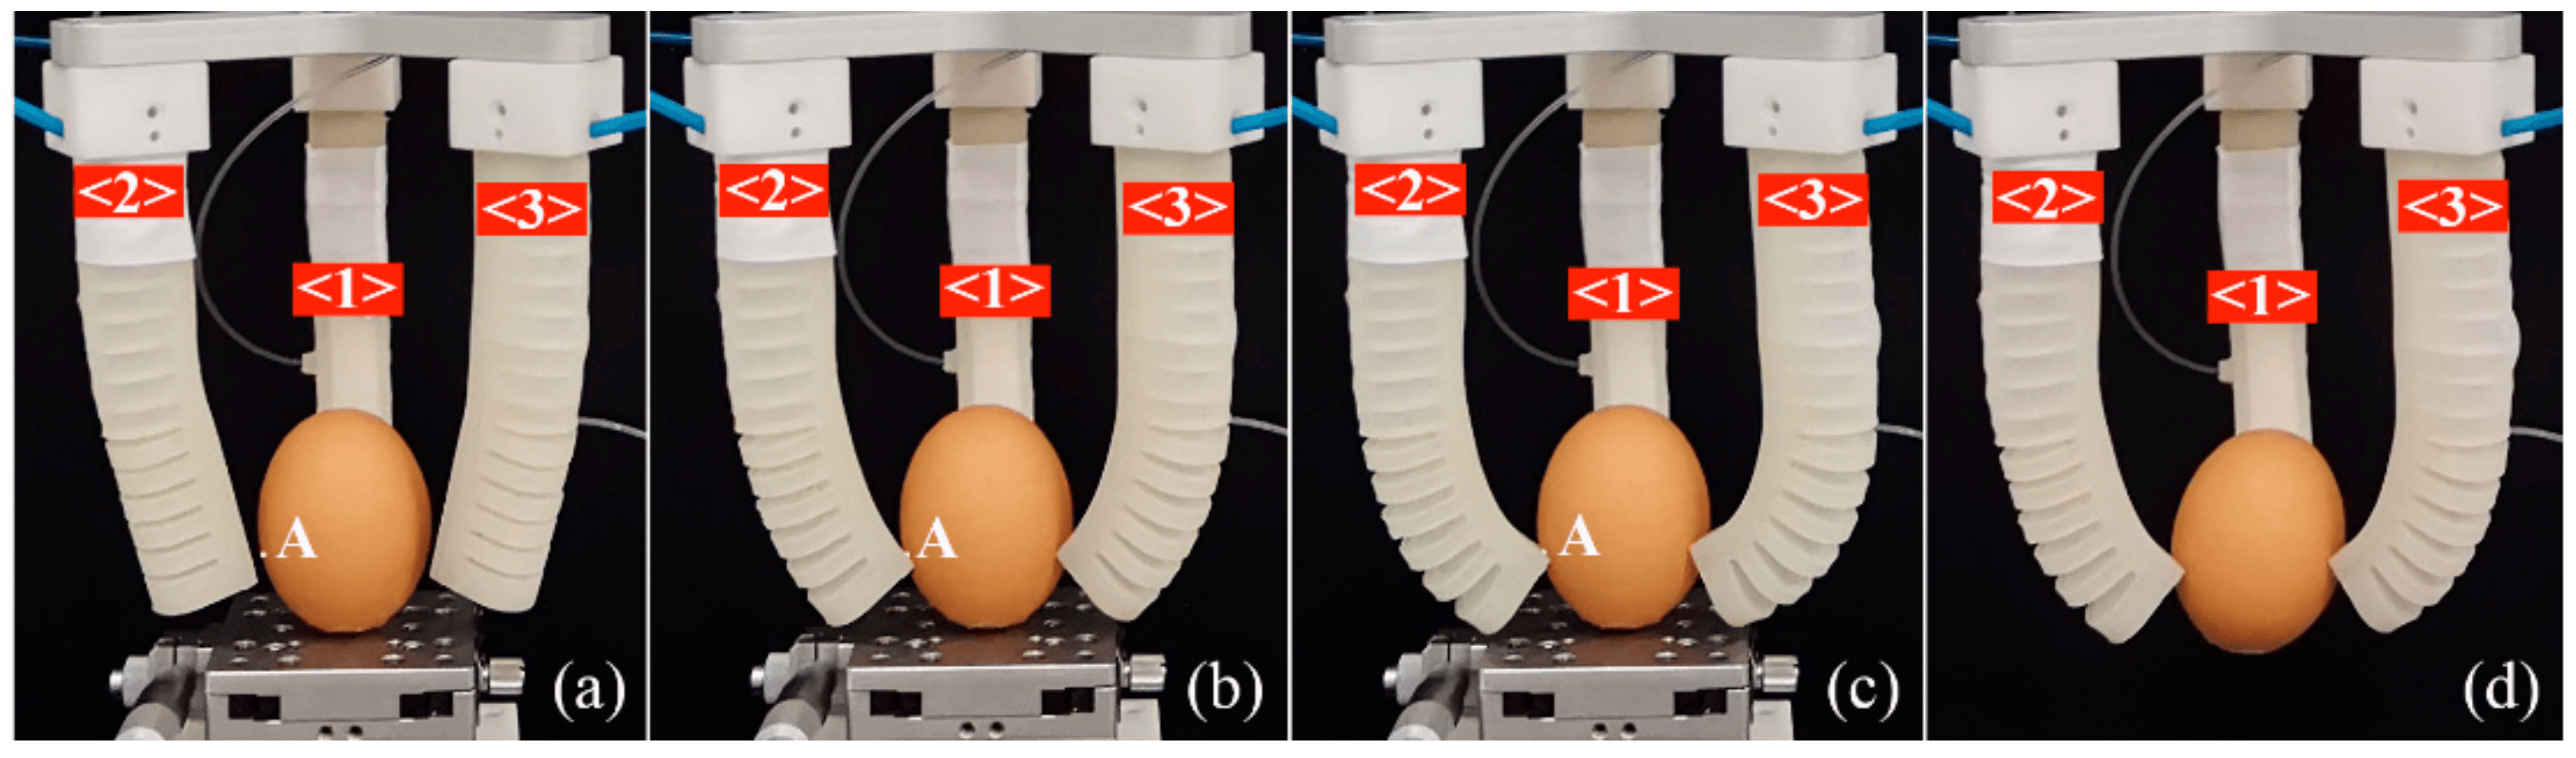
\includegraphics[width=1\columnwidth]{Figures/sensors-22-04851-g014.png}
\caption{Pneumatic actuator grasping process of an egg \cite{yu2022modeling}: (a) The soft actuator moves toward the egg when pneumatic module one is pressurized to 10 kPa, with module two remaining at zero pressure. (b) Contact between the tip of the soft actuator and the egg occurs when the pressure in module one is increased to 20 kPa and module two is set to 14.1 kPa. (c) The egg is securely pinched by the gripper when both module one and module two are pressurized to 20 kPa. (d) The egg is held firmly when the supporting platform is removed, indicating a stable grasp by the gripper.}
\label{linkage structure A}
\end{minipage}
% \qquad
% \begin{minipage}[t]{0.5\textwidth}
% \centering
% \includegraphics[width=0.7\columnwidth]{Figures/linkage structure B.png}
% \caption{Parallel Four-bar Linkage B}
% \label{linkage structure B}
% \end{minipage}
\end{tabular}
\end{figure}

On the other hand, Chameleon-like shooting manipulator offer extended working ranges but suffer from lower success rates and reduced effective working ranges \cite{mochiyama2015chameleon}. Such systems often rely heavily on complex control algorithms and precise timing, which can be difficult to manage in real-time applications, leading to potential delays and reduced effectiveness in fast-paced environments.

\begin{figure}[htbp]
\centering
\begin{tabular}{cc}
\begin{minipage}[t]{0.45\textwidth}
\centering
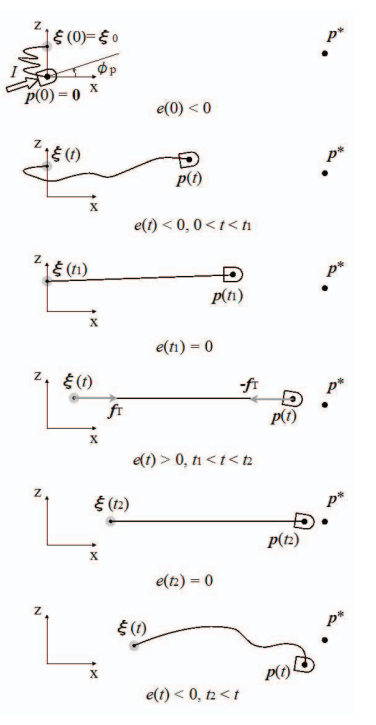
\includegraphics[width=0.8\columnwidth]{Figures/chameleon.png}
\caption{Manipulating model of chameleon-like gripper \cite{mochiyama2015chameleon}.}
\label{linkage structure A}
\end{minipage}
% \qquad
% \begin{minipage}[t]{0.5\textwidth}
% \centering
% \includegraphics[width=0.7\columnwidth]{Figures/linkage structure B.png}
% \caption{Parallel Four-bar Linkage B}
% \label{linkage structure B}
% \end{minipage}
\end{tabular}
\end{figure}

Fractal grippers, as discussed by Tisdale and Burdick, draw inspiration from an older concept called the Fractal Vise \cite{tisdale2023fractal}. Their work emphasizes the gripper's ability to conform passively to various objects using a single actuator. Nonetheless, while these mechanisms offer synergistic properties and adaptability, their integration with existing systems and capacity for high-load tasks are still limited. The passive nature of these grippers, while beneficial in certain contexts, can also lead to a lack of control over the gripping force, making them unsuitable for tasks requiring precise manipulation of heavy or delicate objects.

\begin{figure}[htbp]
\centering
\begin{tabular}{cc}
\begin{minipage}[t]{1.1\textwidth}
\centering
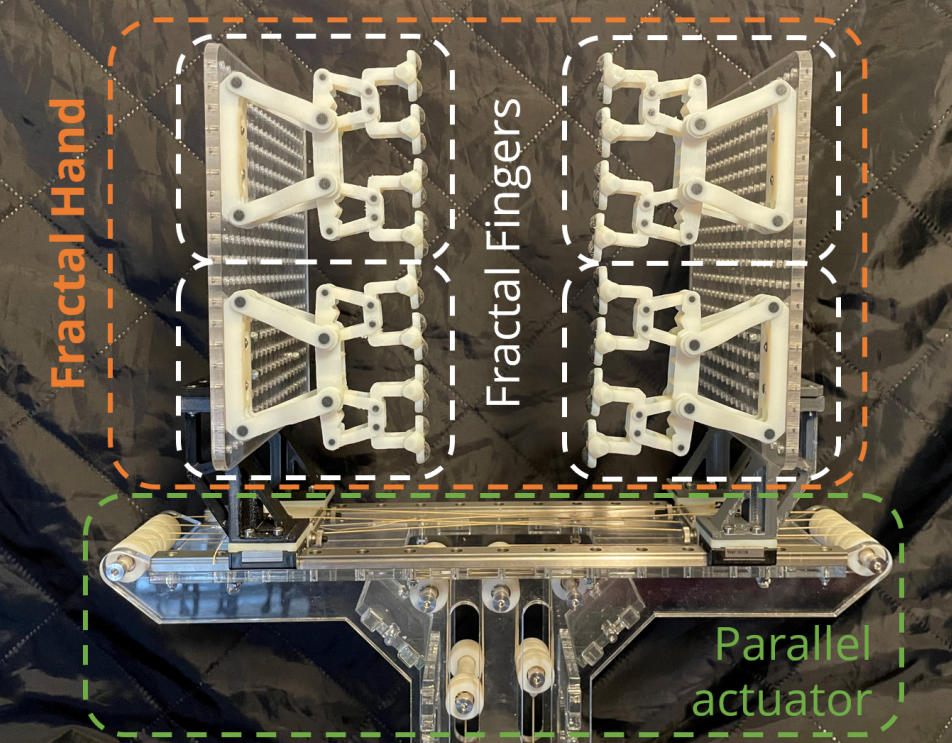
\includegraphics[width=0.8\columnwidth]{Figures/fractal.png}
\caption{ Fractal Hand prototype \cite{tisdale2023fractal}.}
\label{linkage structure A}
\end{minipage}
% \qquad
% \begin{minipage}[t]{0.5\textwidth}
% \centering
% \includegraphics[width=0.7\columnwidth]{Figures/linkage structure B.png}
% \caption{Parallel Four-bar Linkage B}
% \label{linkage structure B}
% \end{minipage}
\end{tabular}
\end{figure}

Lasso Gripper is designed to address these gaps by incorporating a mechanism that can rapidly shoot and retract a string loop, enabling it to capture objects with high speed and precision. Inspired by the traditional lasso used by cowboys and the uurga used by Mongolian herders, this mechanism leverages the structural advantages of a string loop to prevent slippage and ensure a secure grasp. Moreover, Lasso Gripper’s design allows for a large initial capture range, significantly increasing the probability of successful grasping, particularly with fast-moving targets.

Brun et al. provide an insightful analysis of the mechanics of the lasso, illustrating how the rope's shape remains stable in the rotating reference frame of the hand, with line tension balanced by centrifugal force and the rope's weight \cite{brun2014introduction}. This fundamental understanding of lasso mechanics informs the design and functionality of Lasso Gripper, ensuring that it can operate effectively under dynamic conditions.

This research will delve into the design and working principles of Lasso Gripper, discussing its overall structure, the specifics of the string shooting-retracting mechanism, and additional design innovations within the gripper. We will also explore the grasping algorithm, which utilizes depth camera scanning and point cloud analysis to accurately locate and secure the target object. Furthermore, we will design experiments comparing Lasso Gripper’s performance with other gripping mechanisms, highlighting its advantages in various scenarios.

\let\cleardoublepage\clearpage
%%%%%%%%%%%%%%%%%%%% Chapter 3
\chapter{Lasso Gripper: Design, Analysis, and Experiments}

\begin{chaptersummary}
This chapter presents Lasso Gripper as the primary mechanism study and principal novel end-effector concept of this thesis. It is used to investigate tendon-driven design principles and evaluate the feasibility of a controllable tensile loop as a practical robotic end-effector. The concept was inspired by the observation of a toy that launches a flexible string into the air, where manual motion can alter the loop shape and occasionally produce a relatively stable free-space loop. This observation motivated the conversion of a projected loop into an actively retractable capture mechanism. The chapter covers the device concept, mechanical architecture, actuation and sensing design, grasp planning strategy, and a series of demonstration experiments, while also analyzing the fundamental dynamics governing the formation and stability of the self-supporting string loop that enables the gripper to operate.

An analytical model based on a Frenet-Serret formulation is developed to describe the loop behavior by balancing tension, gravity, and aerodynamic drag, allowing identification of loop-formation regimes and critical transition points. Key assumptions and simplifications, including negligible string radius and linear drag approximation, are explicitly stated, and representative experimental observations are used to validate the predicted trends. Together, the modeling and experimental analyses reveal mechanism-level advantages, operational constraints, and potential failure modes that inform the broader thesis on tendon-driven robotic systems.

The experimental program is demonstration-focused and qualitative by design, illustrating the gripper's operating behaviors, tolerance to object uncertainty, and comparative advantages over a conventional antipodal gripper. Comprehensive quantitative evaluation, including large-sample success-rate analysis, repeatability assessment, and detailed parametric sensitivity studies is beyond the scope of this chapter and is recommended for future work.
\end{chaptersummary}
% ------------------------- 2.1 Overall Structure -------------------------
\section{Concept and Design Requirements}

\subsection{Design Inspiration and Concept Formation}

The initial inspiration for Lasso Gripper came from a toy rather than from a conventional robotic gripper. The toy could launch a length of string into the air. By moving the handheld part, the user could change the shape of the airborne string loop, and under certain motions the loop could appear relatively stable for a short period. The toy itself was not a grasping device, and it did not actively tighten around objects. However, the observed phenomenon suggested an important mechanism idea: a flexible string can form a controllable spatial loop when its motion, gravity, aerodynamic drag, and internal tension are appropriately balanced.

This observation was abstracted into a robotic design question. If an airborne loop can be produced in a repeatable way, and if the loop can subsequently be retracted under controlled tension, then the loop may act as a projected capture region rather than a conventional pair of rigid fingers. The robotic concept therefore adds two functions that the toy did not provide: controlled launch and active retraction. Launch creates the open loop in free space, while retraction converts loose enclosure into holding force.

The key mechanism transition is from \emph{free-space loop formation} to \emph{loop-based grasping}. In the toy, the loop is mainly a dynamic visual and physical phenomenon. In Lasso Gripper, the same type of loop is treated as a temporary end-effector geometry. The loop first increases the region in which an object can be captured, and the tightening stage then transforms this region-level interaction into a stable grasp or hold. This design path is important because it separates the source of inspiration from the final robotic function: the contribution is not the toy itself, but the conversion of a free string loop into a controllable capture-and-retraction mechanism.

\subsection{Design Requirements for Robotic Loop Capture}

Translating the toy-inspired phenomenon into a robotic gripper required several design requirements. First, the device had to create a capture region larger than the physical body of the end-effector. This requirement distinguishes Lasso Gripper from parallel-jaw grippers, whose effective capture area is limited by jaw opening and fingertip placement. Second, the loop had to tolerate object-position uncertainty. The intended advantage of the mechanism is not high fingertip precision, but the ability to sweep a loop across a broader target region and then tighten around a useful feature.

Third, the string had to remain light enough for rapid launch and free-space loop formation. A heavy string would sag quickly and reduce the projected capture envelope. Fourth, the string surface had to provide enough interaction with both the driving wheels and the surrounding air. Sufficient wheel friction is needed for repeatable propulsion, while aerodynamic drag contributes to the self-supporting loop behavior analyzed later in this chapter. Fifth, the mechanism had to include active retraction, because a loop that can only be launched cannot reliably generate holding force. Finally, the distal structure had to remain mechanically simple so that the system could be mounted on a robot arm without adding heavy or bulky fingers at the interaction point.

\begin{description}[style=standard, leftmargin=1.5em, labelindent=0pt, itemsep=0.6em]
    \item[\textbf{Large capture envelope:}] The loop should create an interaction region larger than the rigid body of the gripper.

    \item[\textbf{Tolerance to pose uncertainty:}] The mechanism should not require precise antipodal contact placement before capture.

    \item[\textbf{Low string mass:}] The string should be light enough to form a free-space loop during launch rather than immediately collapsing under gravity.

    \item[\textbf{Sufficient friction and aerodynamic interaction:}] The string should be rough enough for reliable friction-wheel propulsion and should interact with air strongly enough to support loop formation.

    \item[\textbf{Active retraction:}] The mechanism must tighten the loop after placement so that enclosure can become a stable grasp.

    \item[\textbf{Low distal complexity:}] The gripper should keep the capture structure flexible and lightweight, with actuation and sensing located proximally where possible.
\end{description}

\subsection{String Material Screening}

Early qualitative trials were conducted to evaluate both string behavior and wheel-string interaction. Candidate string materials included cotton string, fishing line, nylon line, and silicone cord. These trials were used as design screening rather than formal experiments. They were not recorded with video or image documentation and are therefore not treated as quantitative validation evidence. Their purpose was to identify a string and launch-interface combination that could be driven reliably, form a visible and controllable loop, and retract without excessive tangling or slipping.

The original toy used ABS launching wheels. Their surface friction was insufficient under some string conditions, and slipping could occur during launch. Silicone cord was therefore considered because its compliant and high-friction surface could improve engagement with the wheels. However, the silicone cord was too heavy for the desired free-space loop behavior and was less suitable for rapid launch. This observation separated the design problem into two parts: the string should remain light and flexible, while the launching wheel should provide sufficient surface grip. Fishing line was relatively smooth and tended to retain curvature, making it less suitable for stable loop formation. Nylon line was also comparatively smooth, which reduced the reliability of wheel-string interaction. Cotton string provided the best practical balance in the prototype trials. It was light, flexible, and sufficiently rough to interact with both the launch mechanism and the surrounding air. The later prototype therefore used cotton string together with patterned TPU launching wheels, as described in the mechanical design, to improve propulsion reliability without increasing string mass.

This material choice is closely related to the mechanism principle. The string is not merely a passive connector; it is the temporary grasping structure. Its mass, surface texture, flexibility, and bending behavior directly influence launch consistency, loop stability, retraction behavior, and object contact. Therefore, string material selection is part of the mechanism design rather than a secondary implementation detail.

\section{Prototype Architecture and Working Mechanism}

After defining the design requirements, this section describes how the prototype realizes the loop-based grasping concept in hardware. The discussion first presents the system architecture, then explains the capture mechanism, the string shooting and retraction unit, and the controller and sensing hardware that execute the grasping sequence.

\subsection{Overall Prototype Architecture}

\begin{figure}[htbp]
\centering
\begin{tabular}{cc}
\begin{minipage}[t]{0.9\textwidth}
\centering
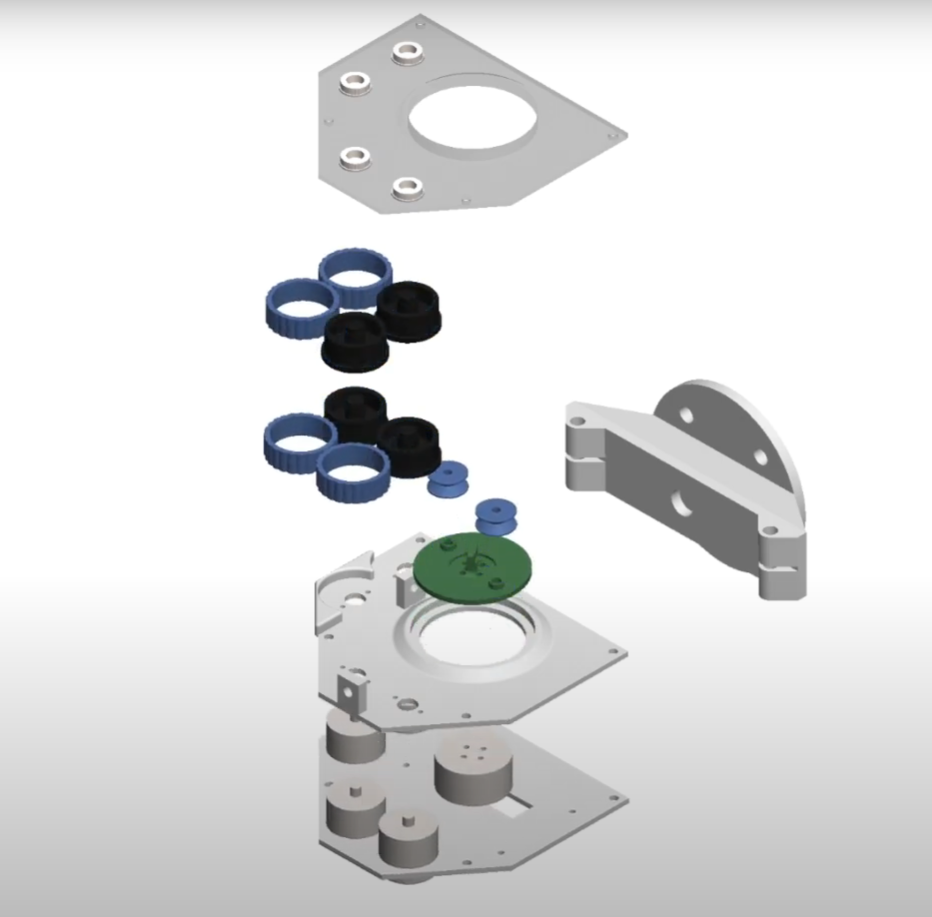
\includegraphics[width=\linewidth]{Figures/overall_img.png}
\caption{The SolidWorks designed hardware of the proposed gripper}
\end{minipage}
\end{tabular}
\end{figure}

Lasso Gripper integrates four core subsystems: the launch-and-retract end-effector, a proximal control unit, sensing for tension and loop position, and a host robot for gross positioning. The end-effector implements the friction-wheel propulsion and spool retraction mechanisms; the control unit coordinates motor commands and processes sensor feedback; sensing includes a spool-mounted force sensor and motor/position encoders used for tension regulation; the host robot provides coarse positioning and aiming for capture. This modular decomposition clarifies subsystem responsibilities and guides the experimental evaluation reported below.

\begin{figure}[htbp]
\centering
\begin{tabular}{cc}
\begin{minipage}[t]{0.9\textwidth}
\centering
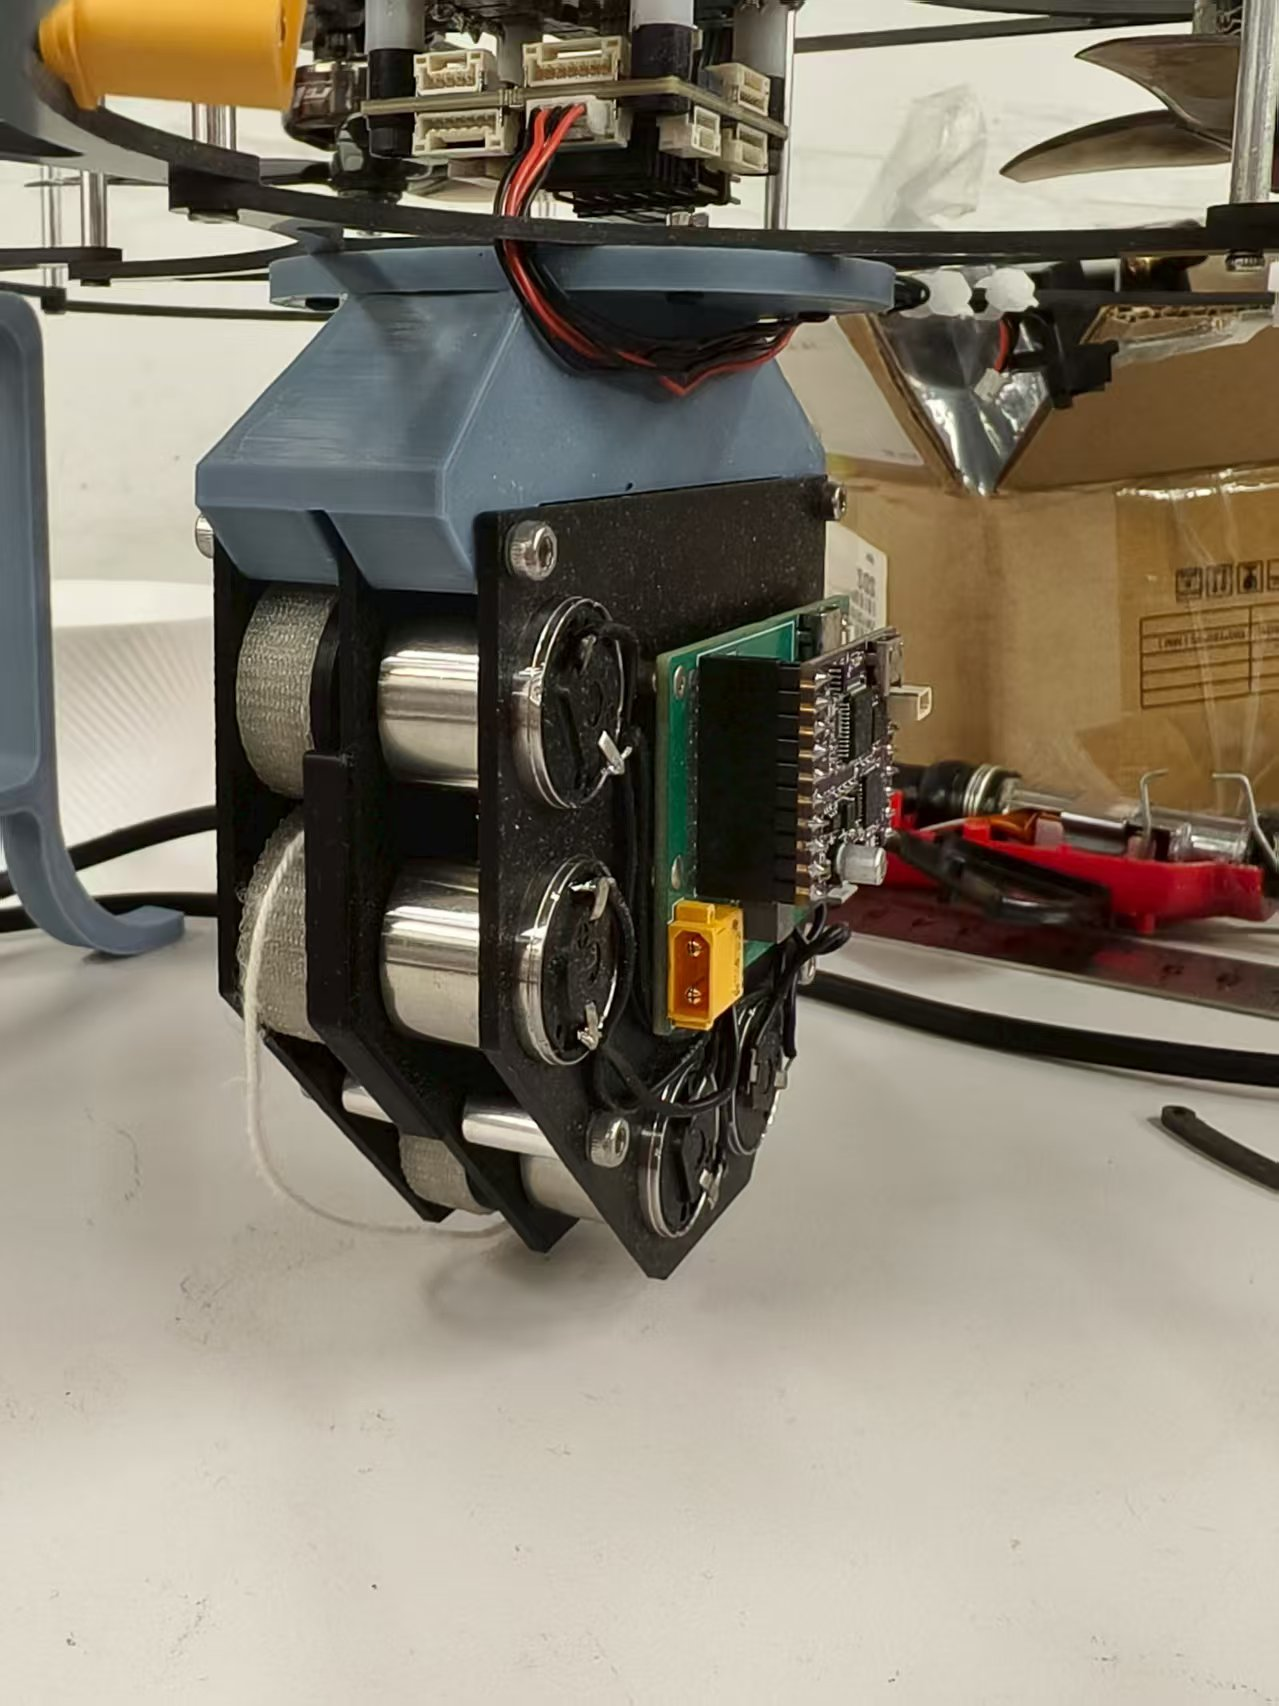
\includegraphics[width=\linewidth]{Figures/system_overview.jpg}
\caption{The proposed gripper connected with an ESP32 controller, motor electronic speed controller.}
\end{minipage}
\end{tabular}
\end{figure}

\subsection{Mechanism of Loop-Based Capture}

The grasping principle of Lasso Gripper differs from classical antipodal grasping. A parallel-jaw gripper typically requires two suitable contact regions and relatively accurate fingertip placement. Lasso Gripper first creates a projected loop, which acts as a large capture envelope. If the loop passes around a neck, protrusion, frame, or enclosed region of the target, subsequent retraction can convert the loose loop into a tightened contact path.

This process can be understood in three phases. In the deployment phase, the launched string forms an open loop in free space. In the enclosure phase, the robot motion or target motion causes the object to enter the loop region. In the tightening phase, the spool retracts the string and increases tension, causing the loop to close around the target. The result is not a two-point contact grasp but a distributed contact interaction along part of the string path.

This distributed contact is the main source of the gripper's advantage for deformable, oversized, and irregular objects. For a deformable object, the string can spread contact over a longer path and reduce local pressure compared with rigid fingertips. For a frame-like object, the loop can pass through or around an opening and then tighten on the frame. For an oversized object, the loop can partially enclose or hook a useful region even when the object is larger than the rigid body of the gripper. For a moving object, the open loop increases the temporal and spatial window for capture, provided that launch and retraction timing are selected appropriately.

The mechanism also has inherent limitations. A loop that misses the target region cannot generate grasping force. A loop that tightens above an unstable center-of-mass relationship can slip during lifting. Excessive retraction can damage soft targets, while insufficient retraction can leave the object unsecured. These limitations motivate the control assumptions, parameter selection, and failure analysis presented later in this chapter.



% ------------------------- 2.2 String Shooting and Retraction Mechanism -------------------------
\subsection{String Shooting and Retraction Mechanism}

The string shooting and retraction mechanism is a defining feature of Lasso Gripper, enabling it to perform complex gripping tasks with high efficiency. The mechanism comprises multiple components working in unison to achieve precise control over the string's movement.

The propulsion of the string is achieved through two pairs of friction wheels. These wheels are designed with high-friction surfaces to grip the string effectively. The wheels are driven by coreless motors with high speed so that the required rotational speeds for rapid string extrusion can be achieved\cite{murata2024elastic}.

During the string shooting phase, both pairs of friction wheels rotate in the same direction, propelling the string forward through a guided track. This track is designed to help the string form a loop within the desired dimensions and shape. In the prototype reported here, the launch duration and wheel speeds were specified by the experiment script rather than adjusted by online visual recognition.

\begin{figure}[htbp]
\centering
\begin{tabular}{cc}
\begin{minipage}[t]{0.9\textwidth}
\centering
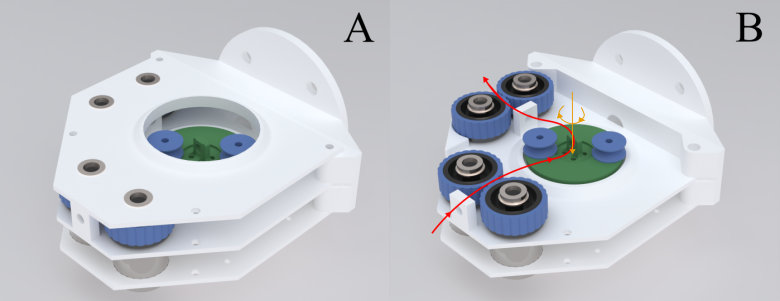
\includegraphics[width=\linewidth]{Figures/Figure11.png}
\caption{The friction wheels and the retraction mechanism driving motors are highlighted for illustration.}
\end{minipage}
\end{tabular}
\end{figure}

When retraction is required, the mechanism undergoes a coordinated sequence of actions. The rear pair of friction wheels maintains its rotational speed, continuing to pull the string inwards. Simultaneously, the front pair of wheels reverses direction, creating a counterforce that pulls the string loop into the space between the two pairs of wheels. This space is precisely designed to accommodate the retracted string without entanglement.

Within this confined space, a spool mechanism is designed. The spool is equipped with a rotational motor that winds the string onto itself, storing it neatly for future use. The tension exerted on the string during retraction is monitored by a force feedback sensor located on the spool's axle. This sensor is used to observe cable loading and support safety limits during the preprogrammed retraction sequence.

\subsection{Controller, Actuation, and Sensing Hardware}

The ESP32 main controller serves as the central hub for Lasso Gripper operations. It receives the experiment script or operator command, sends motor commands to the launch and retraction modules, and reads the sensing signals used for monitoring.
\begin{figure}[htbp]
\centering
\begin{tabular}{cc}
\begin{minipage}[t]{0.5\textwidth}
\centering
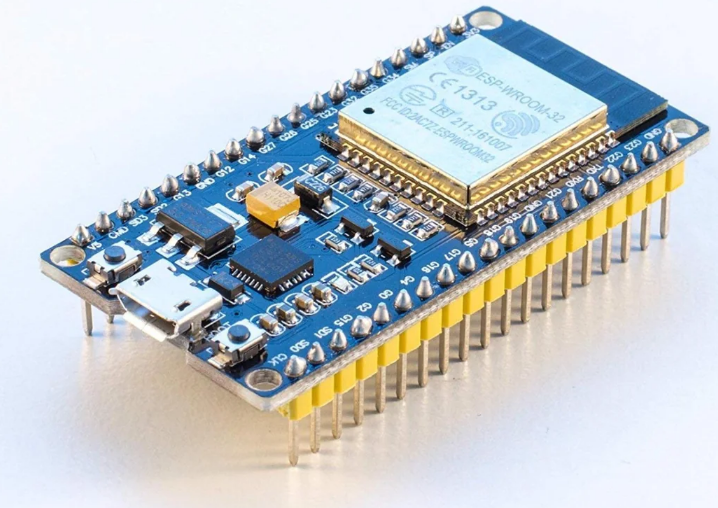
\includegraphics[width=\linewidth]{Figures/esp32.png}
\caption{ESP32 controller used in Lasso Gripper.}
\end{minipage}
\end{tabular}
\end{figure}
Its dual-core processor handles motor command execution, basic sensor monitoring, and communication with external devices. The controller interfaces with a spool-mounted force sensor, motor encoders, and any auxiliary trackers used during experiments.

GPIO pins drive the retraction modules and friction-wheel controllers, while PWM outputs provide fine speed control for the propulsion motors. Wireless connectivity is used for logging and remote monitoring via a host computer when required.

\section{Operational Workflow and Control Logic}
The operation of Lasso Gripper in the reported demonstrations was implemented as a preprogrammed launch, approach, retraction, lifting, and release sequence. The system did not autonomously recognize objects or decide when to grasp based on visual detection. Instead, the target position, approach direction, launch timing, retraction duration, and release command were specified before each trial according to the experimental setup. This section clarifies that control logic and distinguishes the implemented demonstration sequence from possible future closed-loop autonomy.

% ------------------------- 3.1 Demonstration Control Assumptions -------------------------
\subsection{Demonstration Control Assumptions}
The experiments were designed to validate the mechanical feasibility of loop-based capture rather than to demonstrate autonomous perception or decision making. Before each trial, the object was placed in a known region and the robot motion was manually selected or preprogrammed so that the open string loop would sweep across the intended capture region. For static targets, the launch and retraction timing were triggered by the experiment script. For moving-object demonstrations, the gripper was held at a fixed pose and the object was manually thrown through the loop during the launch window.

Sensors were used primarily for command execution, monitoring, and post-trial interpretation rather than for autonomous state transitions. Motor controllers provided speed and position control for the friction wheels and retraction spool. The spool-mounted force sensor was used to monitor cable tension and prevent excessive loading during retraction. Camera images and point-cloud examples were used to illustrate feasible loop placement and caging geometry, but the prototype did not use online object recognition to initiate grasping or release actions.

\subsection{Preprogrammed Grasping State Machine}
The demonstration controller can be described as a simple state machine with scripted transitions. The transitions are based on elapsed time, predefined motor commands, robot trajectory waypoints, operator commands, and safety limits rather than automatic visual recognition. The states are:
\begin{itemize}
    \item \textbf{Idle}: the controller waits for an operator start command.
    \item \textbf{Preset}: the target pose, robot sweep path, launch motor current, retraction motor current, and timing parameters are loaded into the experiment script.
    \item \textbf{Launch}: the friction wheels spin up and extrude the string to form the open loop.
    \item \textbf{Approach/Sweep}: for static objects, the robot follows the predefined path so that the loop passes around the target region; for moving objects, the gripper remains fixed while the object enters the loop.
    \item \textbf{Retract/Tighten}: the spool motor retracts the string according to the programmed duration or position command. Tension is monitored to avoid excessive load.
    \item \textbf{Lift/Transport}: after retraction, the robot performs the scripted lifting or transport motion.
    \item \textbf{Release}: the operator or script commands spool unwinding and friction-wheel reversal or relaxation, allowing the loop to reopen and release the object.
    \item \textbf{Recovery}: the string is rewound to the initial configuration and the controller returns to \textbf{Idle}.
\end{itemize}

The corresponding actuation and signal flow is summarized in Fig.~\ref{fig:grasp_release_flow}. The host script sends velocity or position commands to the ESP32 controller. The ESP32 drives the electronic speed controllers for the friction wheels and the spool motor driver for retraction. Sensor feedback is limited to motor state and cable tension monitoring; it does not trigger autonomous grasp initiation in the current prototype.

\begin{figure}[htbp]
\centering
\begin{tikzpicture}[
    node distance=0.5cm,
    every node/.style={font=\small},
    block/.style={draw, rectangle, rounded corners, align=center, minimum width=3.2cm, minimum height=0.85cm},
    arrow/.style={->, thick}
]
\node[block] (idle) {Idle\\operator start};
\node[block, below=of idle] (preset) {Preset trial\\pose, timing, speeds};
\node[block, below=of preset] (launch) {Launch loop\\friction wheels on};
\node[block, below=of launch] (sweep) {Approach / sweep\\predefined robot motion};
\node[block, below=of sweep] (retract) {Retract / tighten\\spool motor command};
\node[block, below=of retract] (lift) {Lift / transport\\scripted robot motion};
\node[block, below=of lift] (release) {Release\\unwind or relax string};
\node[block, below=of release] (recovery) {Recovery\\rewind and reset};

\draw[arrow] (idle) -- (preset);
\draw[arrow] (preset) -- (launch);
\draw[arrow] (launch) -- (sweep);
\draw[arrow] (sweep) -- (retract);
\draw[arrow] (retract) -- (lift);
\draw[arrow] (lift) -- (release);
\draw[arrow] (release) -- (recovery);
\draw[arrow] (recovery.east) -- ++(1.2,0) |- (idle.east);

\node[block, right=4.4cm of retract, minimum width=3.9cm] (monitor) {Monitoring only\\tension, motor state};
\draw[arrow] (retract.east) -- (monitor.west);
\draw[arrow] (monitor.south) |- (release.east);
\end{tikzpicture}
\caption{Preprogrammed grasping and release sequence used in the demonstrations. The current prototype does not autonomously detect objects or trigger grasping from visual feedback; state transitions are commanded by the operator or experiment script, with tension and motor signals used for monitoring and safety.}
\label{fig:grasp_release_flow}
\end{figure}

\begin{figure}[htbp]
\centering
\begin{tabular}{cc}
\begin{minipage}[t]{0.9\textwidth}
\centering
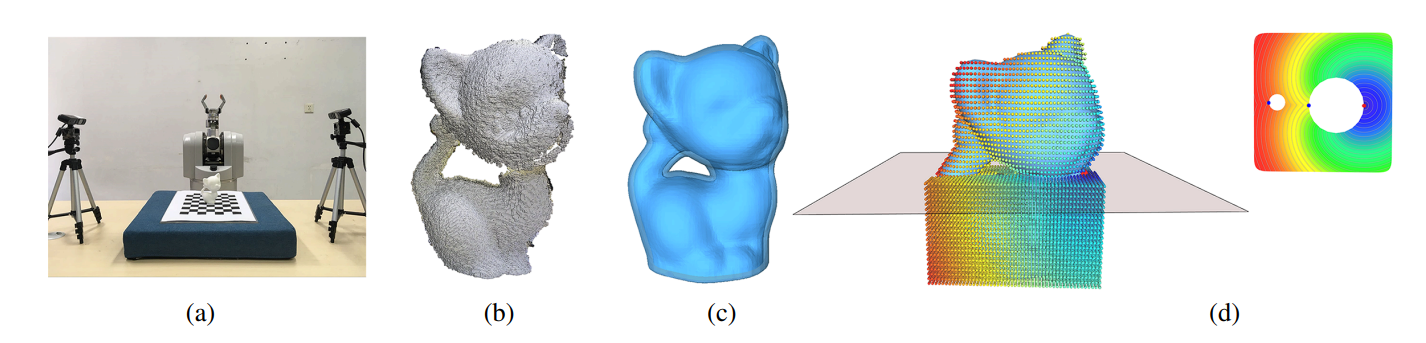
\includegraphics[width=\linewidth]{Figures/caging.png}
\caption{Caging-loop calculation algorithm for Lasso Gripper \cite{liu2018caging}. (a) Setup of the depth reconstruction system. (b) Point cloud captured directly by the depth camera. (c) An r-offset surface built to define the grasping space. (d) Two Morse saddle points (blue) calculated to define the grasping loop.}
\label{fig:caging_loop_method}
\end{minipage}
\end{tabular}
\end{figure}

The caging-loop concept shown in Fig.~\ref{fig:caging_loop_method} motivates the geometric placement of the loop around neck-like regions. In the present prototype, this concept was used to guide experimental setup and qualitative interpretation rather than as a fully automated online perception module. Future versions could integrate the point-cloud caging method with closed-loop planning, but this capability was outside the scope of the current demonstration.

% ------------------------- 3.2 Loop Positioning and Tightening -------------------------
\subsection{Loop Positioning and Tightening}

For the reported experiments, loop positioning was determined before each trial from the known target location and the intended capture region. The key requirement was to align the open loop so that retraction would cause the string to close around a neck, protrusion, or enclosed region of the object. This preplanned positioning was sufficient for demonstrating the mechanical advantages of distributed contact and large capture tolerance.

\begin{figure}[htbp]
\centering
\begin{tabular}{cc}
\begin{minipage}[t]{0.9\textwidth}
\centering
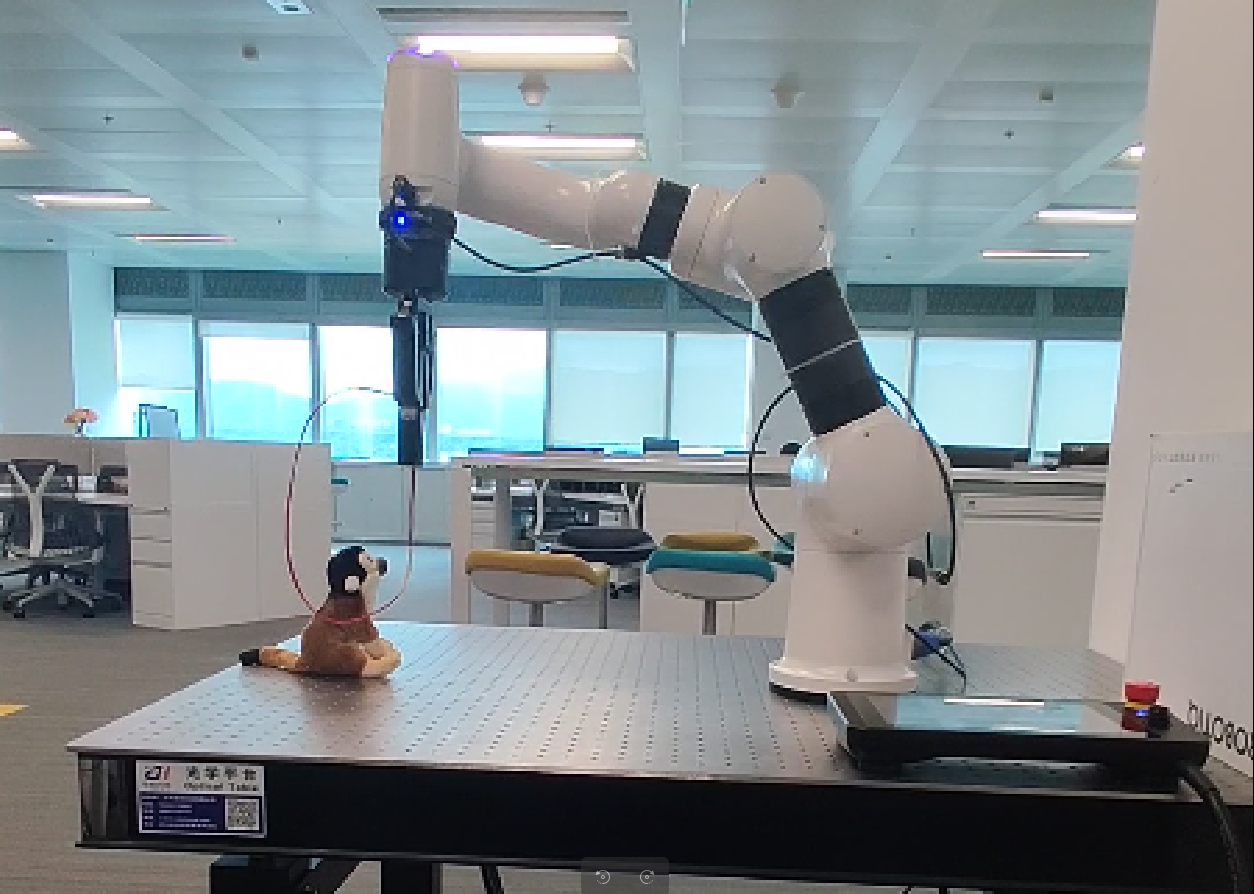
\includegraphics[width=\linewidth]{Figures/exp.png}
\caption{Illustration of the relative position of the string loop and the target object -- an early test}
\end{minipage}
\end{tabular}
\end{figure}

The tightening process is executed in a controlled manner, with the string loop gradually constricting around the target region. The wrist of the gripper approaches the object in synchrony with the programmed retraction action, ensuring that the loop maintains its position and grip.

% ------------------------- 3.3 Real-Time Feedback and Adjustment -------------------------
\subsection{Monitoring and Safety Feedback}
The current prototype uses feedback for monitoring and safety rather than autonomous grasp planning. The spool-mounted force sensor provides cable-tension information during retraction, while motor encoders provide actuator state information. These signals help verify whether the commanded sequence is being executed properly and whether the cable load remains within a reasonable range.

The force feedback sensor, located on the spool's axle, plays a safety role during tightening. If the measured tension exceeds a preset threshold, the controller can stop or relax the retraction command to reduce the risk of damaging the object or overloading the mechanism. In the reported demonstrations, this feedback was not used to automatically recognize successful capture; capture success was assessed from the observed outcome of the trial.

\section{Loop Dynamics and Workspace Extension}

The previous sections define the mechanical sequence used to deploy, position, and tighten the loop. This section explains why the deployed string can form a useful free-space shape and how that shape extends the effective workspace of a robot arm beyond the rigid wrist position.

\subsection{Dynamics of the String Loop}
This section analyzes the loop dynamics that govern Lasso Gripper operation. We focus on the transition from a gravity-dominated regime at low ejection speeds to a self-supporting regime at higher speeds, where aerodynamic drag and inertial effects stabilize the loop shape. The analytic model follows prior theoretical work and is compared with representative experimental profiles to validate qualitative trends \cite{abello2024string}\cite{daerr2019charmed}.

At low ejection speeds the loop sags under gravity. As ejection speed increases, aerodynamic drag and inertial forces can balance gravity and internal tension, yielding a self-supporting loop profile. Characterizing these regimes helps select launch speed, loop length, and control strategies that improve capture reliability.

\begin{figure}[htbp]
\centering
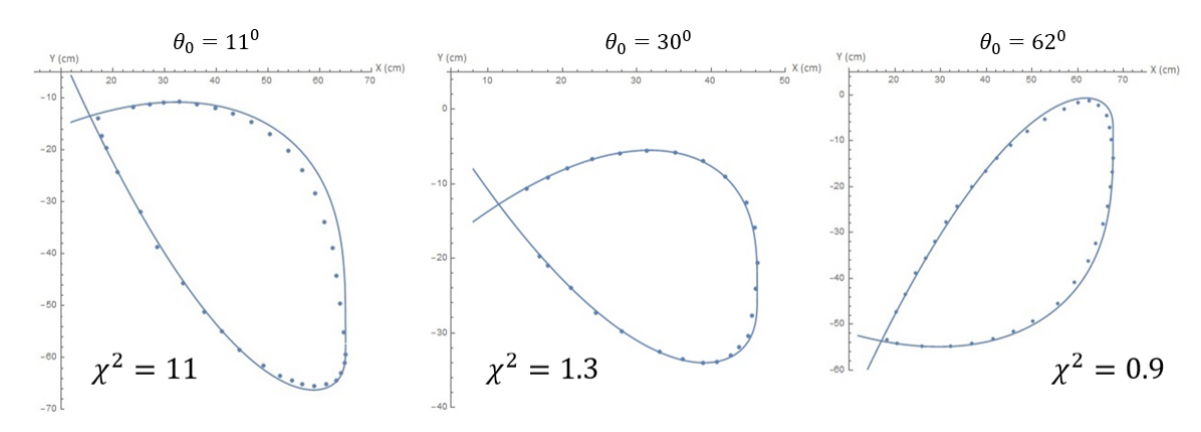
\includegraphics[width=\linewidth]{Figures/stringsim.png}
\caption{Comparison of numerical loop-shape solutions with representative experimental profiles \cite{abello2024string}. Example parameters: linear mass $\mu = 0.283 \pm 0.005\,\mathrm{g\,m^{-1}}$, loop length $L = 160\,\mathrm{cm}$, ejection speed $v = 5.1\,\mathrm{m\,s^{-1}}$, and several ejection pitch angles $\theta_0$. A satisfactory fit with $\chi^2 \leq 11$ was obtained for these samples.}
\label{simulation}
\end{figure}

Assuming the loop junction is at position $s = s_0$ when $t = 0$, the position of the junction along this curve is $s = v \cdot t + s_0 (\mathrm{mod} \, L)$. Denote $T(s)$ as the local tension. The Frenet--Serret frame $(\vec{\tau},\vec{n})$ describes an infinitesimal string element of length $\mathrm{d}s$ subjected to its weight $\mu\,\mathrm{d}s\,\vec{g}$, the local tension $\frac{\mathrm{d}(T\vec{\tau})}{\mathrm{d}s}\,\mathrm{d}s$, and a linear air drag $-f\,\vec{\tau}\,\mathrm{d}s$ with $f>0$.

Newton's motion equation produces:

\vspace{-0.3cm}
\begin{equation}
\begin{split}
\frac{\mathrm{d}(\mu v \vec{\tau})}{\mathrm{d}t} = \mu \vec{g} + \frac{\mathrm{d}(T \vec{\tau})}{\mathrm{d}s} - f \vec{\tau}
\end{split}
\end{equation}

Noting $\mathrm{d}s = v \cdot \mathrm{d}t$ and defining the effective tension $T^o = T-\mu v^2$, the following balance equation can be written:

\vspace{-0.3cm}
\begin{equation}
\begin{split}
T^o \vec{\tau} - f \vec{\tau} +\mu \vec{g}s=\vec{0}
\end{split}
\end{equation}

If the origin is wisely chosen for $\vec{r}$ as the point $o$ where the tangent to the loop is vertical, the integration constants will vanish. In the vertical local Frenet--Serret frame, defining $\tan\theta = \frac{\mathrm{d}z}{\mathrm{d}x}$, the following can be obtained:

\vspace{-0.3cm}
\begin{equation}
\begin{split}
-f \cdot ( x \tan \theta - z )+\mu gs=0
\end{split}
\end{equation}

This integro-differential equation admits analytical solutions under the stated simplifications; representative solutions are compared with experiment in Fig. \ref{simulation}.

The formation of the self-supporting loop is governed by aerodynamic drag acting on the string. Daerr et al. (2019) investigated this drag both experimentally and theoretically, focusing on a smooth long cylinder moving along its axis \cite{daerr2019charmed}. The drag arises from interaction between the moving string and the surrounding air, producing pressure and shear forces that can support the loop.

The loop-shape equations are formulated under the assumption of negligible string radius. They reveal a critical interface separating two regions: a supercritical zone (string speed larger than wave speed) and a subcritical zone (wave speed larger than local string speed). Regular solutions that cross this juncture continuously can be obtained and compared with experimental profiles.

In practical terms, understanding the string loop dynamics has significant implications for Lasso Gripper's design and operation. By leveraging the principles of aerodynamic drag and the transition between different velocity regimes, Lasso Gripper can achieve precise control over the string loop's shape and stability. This enables the gripper to handle objects with varying sizes and shapes effectively, improving robustness of capture.

\subsection{Workspace Analysis}
Because Lasso Gripper forms a self-supporting loop in three-dimensional space, the operational workspace of the proposed manipulator extends beyond the physical reach of the robotic arm.

\begin{figure}[ht]
    \centering
    
\includegraphics[width=0.8\linewidth]{workspace.png} 
    \caption{Lasso Gripper string loop is set at the end of UR5 robotic arm. The green point at the end of the robotic arm marks the position reachable by a rigid manipulator, while the red point indicates the furthest position on the string loop from the original point at the same robotic position.}
    \label{ws1}
\end{figure}

Consistent with the loop-dynamics analysis above, the three-dimensional pose kinematics of the lasso-type end-effector can be characterized by constrained dynamics under gravitational loading. For the local coordinate system constrained by gravity, the working plane is defined as the plane formed by the lasso's ejection direction and the gravity direction. The rotation with the normal vector of this working plane as the rotation axis is defined as pitch, while the rotation with the gravity vector as the rotation axis is defined as yaw. According to the right-hand coordinate system, the roll rotation axis is defined as the axis orthogonal to both the pitch and yaw rotation axes, lying within the working plane. Specifically, the gripper mechanism exhibits negligible roll angular displacement within the global coordinate frame due to gravitational stabilization. Its pitch orientation becomes parametrically dependent on the projectile's ejection velocity vector, while yaw angle variations are governed by the robotic manipulator's pose in Cartesian space.

\begin{figure}[htp]
    \centering
    
\includegraphics[width=0.6 \linewidth]{ws3.jpg} 
    \caption{The initial robotic arm workspace is marked in green, and the extended Lasso Gripper workspace is marked in red.}
    \label{ws2}
\end{figure}

A case study is conducted with specific parameters to investigate the workspace of Lasso Gripper on a 6-axis robotic arm using the Monte Carlo method. A UR5 robot without joint angle limits is used as an example in Fig. \ref{ws1}, and $[R, x_{+}, x_{-}]$ is set as $[0.7, 0.2\,m, 0.1\,m]$ in this case. The green point at the end of the robotic arm is the specific position that a rigid manipulator can reach, and the red point represents the furthest point on the string loop from the same robotic position. The sets of green and red points in Fig. \ref{ws2} are the workspace of the robotic arm and the extended workspace of Lasso Gripper, respectively. After generating 200,000 sampled robotic-arm configurations, the convex-hull workspace volume is calculated. The volume of the original UR5 workspace convex hull is $3.4620\,\mathrm{m^3}$, and the volume of the extended Lasso Gripper workspace convex hull is $8.9002\,\mathrm{m^3}$. The workspace extension ratio reaches $157.08\%$.
\section{Experimental Methodology}

The preceding sections establish the mechanism, control sequence, and loop behavior. The following experiments were designed to evaluate whether these elements can produce useful grasping outcomes under selected demonstration conditions.

\subsection{Experimental Objectives}
To validate the unique capabilities of Lasso Gripper and to compare its performance with antipodal grippers, the following experimental procedure was designed. The setup employed a modular robotic arm (Inovo Robotic) with a maximum payload of 6 kg, mounted on a flat platform where the target objects were placed.
The experimental objectives were divided into four categories:

    \begin{enumerate}
        \item Capturing animal figures by the neck or horns,

        \item Capturing objects of diverse shapes,

        \item Capturing oversized objects through shape adaptation, and

        \item Capturing moving objects.
    \end{enumerate}

\subsection{Experimental Setup}
For Objectives 1 to 3, the procedure consisted of the following steps:

    \begin{enumerate}
        \item The robotic arm moved to a predefined position to initiate the launch phase;

        \item Lasso Gripper was swept toward the target while maintaining its open-loop configuration;

        \item Upon reaching the target, the string was retracted to secure the object;

        \item The arm performed a vertical lifting motion while maintaining a stable grip.
    \end{enumerate}
For Objective 4, the robotic arm remained stationary, and Lasso Gripper independently executed the capture process aimed at intercepting a moving object in flight.
\paragraph{Control mode}
All demonstrations used a preprogrammed control sequence. The system did not autonomously detect the object or decide when to initiate grasping. Instead, the robot path, launch timing, retraction timing, and release timing were defined before each trial. The operator initiated the sequence, and the controller executed the scripted motor commands while monitoring cable tension and motor state for safety.
\subsection{Experimental Procedure}
The experimental procedure was divided into phases to evaluate Lasso Gripper's performance:
\begin{enumerate}
    \item \textbf{Static Object Gripping Tests}: Static object gripping tests were conducted to assess the gripper's ability to handle stationary objects. Test objects were placed in fixed positions, and the preprogrammed launch-and-retract sequence was executed to secure and lift each object. Success rates, gripping forces, and any slippage or deformation of the objects were recorded where feasible.

\item \textbf{Dynamic Object Gripping Tests}: Dynamic object gripping tests focused on evaluating the gripper's performance with moving objects. Test objects with controlled motion, such as rolling or sliding trajectories, were introduced and the lasso attempted to intercept and secure them. The effectiveness and speed of the gripping action were measured to assess performance in dynamic scenarios.

\item \textbf{Comparative Analysis}: Finally, a comparative analysis was conducted to compare Lasso Gripper's performance with traditional gripping methods. Parallel tests using a standard parallel-jaw gripper were carried out on the same set of test objects. Differences in gripping force, handling precision, success rates, and overall efficiency were analyzed to highlight advantages and potential areas for improvement of Lasso Gripper.
\end{enumerate}


\subsection{Data Collection and Analysis}
Data collection involved capturing both quantitative and qualitative metrics where available. Key observations included whether the loop enclosed the intended target region, whether retraction produced a stable hold, whether the object could be lifted or transported, and whether visible damage, deformation, slippage, or entanglement occurred. The spool force sensor provided cable-load information during retraction, while images and video frames were used to interpret loop placement around candidate neck, frame, or protrusion regions. Where feasible, counts of successful and failed grasps were noted; however, the evaluation emphasis in this section is demonstrative rather than a full statistical study.

Limited summary statistics were computed where appropriate, but a comprehensive statistical campaign (large-sample success rates, fatigue tests) was outside the present scope and is recommended for future work. Most representative scenes were repeated twice after the loop length and approach angle had been preset. This trial structure should therefore be interpreted as a repeatability check under selected demonstration conditions rather than as an unbiased statistical evaluation across random object poses.

\begin{table}[htbp]
    \centering
    \caption{Representative Lasso Gripper demonstration cases}
    \label{tab:lasso_demo_cases}
    \begin{tabular}{p{0.18\linewidth} p{0.12\linewidth} p{0.12\linewidth} p{0.16\linewidth} p{0.20\linewidth}}
        \toprule
        Target & Mass & Trials & Outcome & Notes \\
        \midrule
        3D-printed figures & 50\,g & 2 & 2 successful & Horn/neck capture \\
        DJI Mini 3 drone & 249\,g & 2 & 2 successful & Frame capture \\
        Cabbage & 170\,g & 2 & 2 successful & Irregular object \\
        Empty coke can & 305\,g & 2 & 2 successful & Cylindrical object \\
        Chili pepper & 90\,g & 2 & 1 secure, 1 slipped & Unbalanced mass \\
        Oversized balloons & -- & Example & Successful & Adaptive contact \\
        Thrown balloons & -- & Example & Successful & Moving target \\
        \bottomrule
    \end{tabular}
\end{table}

The table summarizes the representative cases used in this chapter. Because the approach angle and loop length were selected before each trial, the results should be interpreted as feasibility demonstrations under known setup conditions rather than as a randomized statistical evaluation. The detailed interpretation of these cases is presented after the experimental results.

\subsection{Experimental Parameter Selection}
Although the demonstrations were not designed as a large statistical campaign, several operating parameters were selected deliberately before each trial. These parameters determine whether the loop forms, reaches the target, tightens in time, and remains stable during lifting. The most important parameters are loop length, launch speed, approach angle, retraction timing, and lifting trajectory.

Loop length defines the size of the capture region. A longer loop increases the geometric tolerance to object-position error and makes it easier to capture oversized objects, but it also increases the risk of sagging, contact with the support surface, and entanglement during retraction. A shorter loop is easier to control and retract, but it requires more accurate placement around the target. For objects with clear neck or horn features, such as the 3D-printed bull and horse figures, a moderate loop length is sufficient because the loop only needs to pass around a narrow capture feature. For balloons or large irregular objects, a larger loop is beneficial because the target may not provide a precise narrow feature.

Launch speed affects whether the loop becomes self-supporting. If the speed is too low, gravity causes the loop to collapse before it sweeps across the target. If the speed is too high, the loop may become difficult to place accurately and may rebound after contact. The selected speed must therefore produce a loop that is large and stable enough for capture but not so aggressive that it destabilizes the approach. This trade-off is consistent with the loop-dynamics analysis presented earlier in the chapter.

Approach angle determines how the open loop intersects the object. For neck-like features, the preferred approach is one in which the loop plane crosses behind the feature and the retraction direction pulls the loop toward a mechanically stable region. For cylindrical or irregular objects, the approach angle must also consider the center of mass. The chili-pepper failure demonstrates this issue: even if the loop initially encloses part of the object, lifting can cause rotation if the tightened loop does not settle below or around a stable support region.

Retraction timing is the transition between geometric capture and force closure. Early retraction can close the loop before the target is fully inside the capture region, producing a miss. Late retraction can allow the target to leave the loop or allow the loop to slide to an undesired position. Retraction speed also matters. A slow retraction may fail to secure moving objects; a fast retraction may cause overshoot, local compression, or string shift. In the current prototype, these timing values were selected manually from preliminary trials and then held constant for the repeated demonstrations.

\begin{table}[htbp]
    \centering
    \caption{Role of main experimental parameters in demonstrations with Lasso Gripper}
    \label{tab:lasso_parameters}
    \begin{tabular}{p{0.20\linewidth} p{0.30\linewidth} p{0.32\linewidth}}
        \toprule
        Parameter & Increasing the parameter tends to & Practical risk if poorly selected \\
        \midrule
        Loop length & Increase capture area and pose tolerance & Sagging, surface contact, entanglement, slower recovery \\
        Launch speed & Improve loop support and reach & Overshoot, rebound, reduced placement accuracy \\
        Approach angle & Change intersection between loop and target feature & Missed capture or unstable tightening region \\
        Retraction delay & Allow target to enter the loop before closure & Late closure and target escape \\
        Retraction speed & Tighten faster and improve moving-object capture & Local compression, string slip, or object rotation \\
        Lifting path & Test whether capture remains stable under load & Slip if loop is not below a stable support region \\
        \bottomrule
    \end{tabular}
\end{table}

These parameters are coupled rather than independent. For example, a long loop may require a higher launch speed to remain self-supporting, but higher speed may require a gentler approach angle to avoid collision or rebound. Similarly, a late retraction may be acceptable for a stationary cabbage but unacceptable for a thrown balloon. For this reason, the current experiments should be interpreted as selected operating demonstrations. They identify feasible parameter combinations and observed failure boundaries, but they do not yet define a complete parameter map.

\subsection{Success Criteria and Failure Taxonomy}
To make the demonstration results interpretable, success was defined as completion of the intended capture-and-lift sequence without object escape or visible damage. A trial was considered successful when the loop enclosed the target region, retraction generated a stable hold, and the robot lifted or transported the object through the scripted motion. A trial was considered partially successful when the loop initially captured the target but the object slipped, rotated out, or could not be transported reliably. A trial was considered failed when the loop missed the target, tangled, or could not close around a mechanically useful region.

This definition is deliberately task-based rather than purely geometric. A loop that touches the object is not necessarily a successful grasp. The loop must also settle into a stable force path that supports the object during lifting. Conversely, the loop does not need to achieve classical antipodal force closure at two precise points. Its advantage is that it can use distributed contact and caging-like enclosure to tolerate uncertainty.

\begin{table}[htbp]
    \centering
    \caption{Failure taxonomy for loop-based capture}
    \label{tab:lasso_failure_taxonomy}
    \begin{tabular}{p{0.22\linewidth} p{0.32\linewidth} p{0.30\linewidth}}
        \toprule
        Failure type & Typical cause & Design or control implication \\
        \midrule
        Geometric miss & Loop does not intersect a valid capture region & Improve approach planning and loop placement \\
        Premature closure & Retraction begins before target enters the loop & Delay retraction or use visual/tension trigger \\
        Late closure & Target leaves the loop before tightening & Shorten delay or increase retraction speed \\
        Slip after capture & Loop settles above center of mass or on low-friction region & Select lower support region or add multi-loop capture \\
        Entanglement & Long loop contacts fixtures, table, or gripper body & Limit loop length and improve recovery path \\
        Excessive compression & Retraction tension is too high for soft targets & Add tension regulation and object-dependent limits \\
        Dynamic escape & Moving target crosses loop too quickly or off-axis & Increase capture window or add tracking feedback \\
        \bottomrule
    \end{tabular}
\end{table}

The taxonomy helps explain why a simple success count would be insufficient at this stage. Two failures may both appear as unsuccessful grasps, but they can require different design responses. A geometric miss suggests a planning or sensing problem. A slip after capture suggests a stability or center-of-mass problem. Excessive compression suggests a tension-control problem. Entanglement suggests a loop-length and recovery-path problem. Distinguishing these categories is necessary before the mechanism can be improved systematically.

\section{Experimental Results}
% (paragraph will be indented)
The evaluation reported in this section is demonstration-focused and intended to validate feasibility, illustrate common operating modes, and highlight comparative behavior versus conventional antipodal grasping. Test cases emphasized scenarios where a loop-based capture offers clear mechanical advantages. Results are presented as illustrative sequences and representative frames rather than as full statistical studies. Observed failure modes (entanglement, missed captures at extreme approach angles, and tension-management lapses) are documented to guide design improvements.
\subsection{Various Objects Grasping Results}
\begin{figure}[htbp]
    \centering
    
\includegraphics[width=0.7 \linewidth]{test3.png}
    \caption{Validation of grasping ability via bull and horse figures.}
    \label{fig:3}
\end{figure}

\begin{figure}[htbp]
    \centering
    
\includegraphics[width=0.7 \linewidth]{test1.png}
    \caption{Validation of grasping ability over variable shapes: drone, cabbage, coke can and chili pepper.}
    \label{fig:4}
\end{figure}

\begin{figure}[htbp]
    \centering
    
\includegraphics[width=0.7 \linewidth]{test2.png}
    \caption{Validation of grasping ability with oversized objects: inflated balloons.}
    \label{fig:5}
\end{figure}
Fig. \ref{fig:3} illustrates the experimental results for Objective 1. The lasso attached to the horns and necks and secured the figures, allowing the robot to lift and transport them from the platform. These approximately 50\,g figures were useful because the horn and neck features provided repeatable geometric regions for loop closure. For the second set of target objects (a drone, a cabbage, an empty coke can, and a chili pepper), Lasso Gripper was tested on objects with more varied geometry and mass. The drone weighed approximately 249\,g, the cabbage approximately 170\,g, the empty coke can approximately 305\,g, and the chili pepper approximately 90\,g. Under the preset loop length and approach angle, the drone, cabbage, and coke-can cases were each completed successfully in two repeated trials. The chili pepper was less stable: one trial slipped out of the loop after capture because its mass distribution was uneven and the loop tightened around a region that did not remain below the center of mass during lifting.
\begin{figure}[htbp]
    \centering
    
\includegraphics[width=0.7 \linewidth]{test4.png}
    \caption{Flying object is captured by Lasso Gripper.}
    \label{fig:6}
\end{figure}
The grasping strategy for these experiments was similar. In both cases, the robot swept above the target while Lasso Gripper maintained the string in its full range, ensuring that the target could be captured as the string retracted. This strategy was extended to expansive targets such as oversized balloons. The third set comprised two flower-shaped balloons (diameters 45 cm and 71 cm) and a spike ball of 18 cm diameter, as shown in Fig. \ref{fig:5}. Although Lasso Gripper could not fully encircle the largest balloons due to loop-size limitations, the loop still secured them sufficiently to lift them from the platform. This observation led to the fourth case, capturing flying objects. Fig. \ref{fig:6} shows examples where a long balloon and a small flower balloon were manually thrown through Lasso Gripper's loop and successfully intercepted.

Some notable phenomena were observed during the demonstrations, illustrating additional advantages of Lasso Gripper. The string's sustained high speed made it possible to grasp objects placed close to surfaces. In Fig. \ref{fig:4} (B) and (D), where the cabbage and chili pepper were placed near the table, Lasso Gripper maintained the loop shape and achieved successful grasps despite limited clearance between the object and support surface. The adaptive, distributed contact provided by the loop tolerated deviations in placement; compared with the grasp posture in Fig. \ref{fig:5} (D), the loop in Fig. \ref{fig:5} (C) exhibited an unexpected pose deviation yet still produced a secure grip. Thus, Lasso Gripper demonstrates adaptive force-closure behavior.

The failure modes observed in the demonstrations were also informative. First, the loop may miss the target if the preset approach path does not sweep across a valid caging region. Second, even when the loop initially catches the object, a strongly unbalanced target can rotate during lifting and shift the loop toward an open end, as observed in the chili-pepper case. Third, excessive retraction can produce unnecessary local compression on soft objects, while insufficient retraction may leave the loop too loose for transport. These limitations motivate future closed-loop planning and tension regulation, but they do not undermine the main mechanism result: a simple tensile loop can provide a large capture region and distributed contact without requiring precise antipodal point placement.

\subsection{Comparison with Antipodal Point Gripper}

\begin{figure}[htbp]
    \centering
    
\includegraphics[width=0.7 \linewidth]{compare.png}
    \caption{The inflated balloon is captured by the antipodal gripper. As a result of the concentrated stress applied, the balloon was severely deformed.}
    \label{fig:7}
\end{figure}
As the comparison group, the 2F-140 gripper from Robotiq was used as the classical antipodal gripper. In this scenario, the small flower balloon served as the target due to its elasticity. As shown in Fig. \ref{fig:7}, the flower balloon experienced severe deformation when grasped by the antipodal gripper. Although the balloon remained intact after the trial, the limitation of traditional grippers for delicate or highly deformable objects was evident. Instead of concentrating forces on small contact patches, Lasso Gripper captures objects via distributed rope tension, avoiding damage to delicate surfaces and enabling handling of larger, potentially heavier objects than some traditional grippers.

\section{Discussion and Mechanism-Level Implications}

\subsection{Interpretation of Demonstration Evidence}

The experimental evidence in this chapter should be read as mechanism validation. The goal is to show that a launched tensile loop can create capture behaviors that are difficult for conventional point-contact grippers. The results are not intended to prove deployment-level reliability. This distinction matters because Lasso Gripper has a large operating space: object shape, object mass, center-of-mass location, surface friction, target motion, loop length, launch speed, approach direction, retraction timing, and lifting trajectory can all affect the outcome.

The demonstrations nevertheless support several specific claims. First, loop-based capture can use object features that are not suitable for antipodal grasping. Horns, necks, drone frames, and irregular vegetable surfaces all provide candidate regions for loop closure. Second, distributed contact can reduce local deformation compared with point-contact grasping, as illustrated by the balloon comparison. Third, the gripper can interact with targets that exceed the convenient opening range of a parallel-jaw gripper because the functional capture region is defined by the deployed loop rather than by rigid jaw spacing. Fourth, the same mechanism can capture both stationary and moving objects when the timing is preset appropriately.

\begin{table}[htbp]
    \centering
    \caption{Evidence interpretation for representative target categories}
    \label{tab:lasso_evidence_interpretation}
    \begin{tabular}{p{0.22\linewidth} p{0.30\linewidth} p{0.30\linewidth}}
        \toprule
        Target category & Mechanism behavior demonstrated & Remaining validation gap \\
        \midrule
        Horned and necked figures & Capture using protrusions and enclosed regions & Randomized pose and feature-size tolerance \\
        Drone frame & Capture of sparse frame-like geometry & Robustness to propeller guards, cables, or fragile components \\
        Cabbage and coke can & Handling of irregular or cylindrical objects & Surface-friction and mass-distribution sensitivity \\
        Chili pepper & Identification of slip due to asymmetric mass distribution & Stable capture planning around center of mass \\
        Oversized balloons & Distributed contact over targets larger than rigid gripper opening & Tension limits for fragile deformable objects \\
        Thrown balloons & Moving-target interception under preset timing & Closed-loop tracking and automatic trigger timing \\
        \bottomrule
    \end{tabular}
\end{table}

The results therefore justify the mechanism concept and motivate a more quantitative next phase. Future experiments should randomize object pose and approach direction, repeat each condition over larger trial counts, and record loop state, cable tension, object motion, and failure category. A meaningful quantitative campaign would report not only success rate but also the parameter boundary at which the loop transitions from reliable capture to miss, slip, or entanglement.

\subsection{Comparison Criteria for Loop and Antipodal Grippers}

The comparison between Lasso Gripper and the Robotiq 2F-140 gripper is qualitative, but it can still be framed using explicit criteria. A parallel-jaw gripper is strong and repeatable when it can place its fingertips at suitable contact points. Its main limitation appears when the object is too large, too deformable, moving, or difficult to access from two opposing sides. Lasso Gripper has the opposite profile. It does not provide the same precise fingertip placement, but it can define a larger capture region and distribute contact through a flexible loop.

This difference means that the two grippers should not be evaluated only by peak grip force. For deformable or fragile targets, a high local grip force can be undesirable. For oversized targets, jaw opening may be more limiting than motor force. For moving targets, capture-region size and timing may matter more than fingertip accuracy. For frame-like objects, the ability to pass through or around an opening can be more important than surface friction.

\begin{table}[htbp]
    \centering
    \caption{Qualitative comparison criteria for Lasso Gripper and antipodal grippers}
    \label{tab:lasso_antipodal_criteria}
    \begin{tabular}{p{0.24\linewidth} p{0.29\linewidth} p{0.29\linewidth}}
        \toprule
        Criterion & Lasso Gripper tendency & Antipodal gripper tendency \\
        \midrule
        Capture region & Large, loop-defined, tolerant to moderate pose error & Limited by jaw opening and fingertip placement \\
        Contact distribution & Distributed along string-object contact path & Concentrated at two main contact patches \\
        Deformable-object handling & Can reduce local deformation if tension is limited & Can deform object under high local pressure \\
        Oversized-object handling & Possible if loop can partially enclose or hook feature & Limited by maximum jaw opening \\
        Moving-object capture & Possible with large loop and correct timing & Requires accurate tracking and fingertip placement \\
        Precision placement & Lower, because loop shape is flexible & Higher when object geometry is known \\
        Failure mode & Miss, slip, entanglement, excessive loop tension & Missed fingertips, crushing, slipping from point contacts \\
        \bottomrule
    \end{tabular}
\end{table}

This comparison clarifies the intended contribution. Lasso Gripper is not proposed as a universal replacement for antipodal grippers. It is a complementary end-effector for tasks where capture tolerance, distributed contact, and geometric enclosure are more valuable than precise fingertip placement.

\subsection{Mechanism Contribution of Lasso Gripper}

Work on Lasso Gripper provides the main mechanism contribution of this thesis and offers several insights that generalize beyond the specific prototype. First, the principle of using a flexible tensile element to create an adaptive capture region suggests new ways to trade capture range for control complexity. Second, proximal actuation enables low distal mass while still producing useful end-effector behavior through a flexible transmission path. Third, performance metrics such as capture probability, peak tensile load, retraction dynamics, and hysteresis in the string path form a compact evaluation set that is applicable to other tendon-driven designs.

Taken together, these demonstrations support the feasibility of Lasso Gripper as a novel end-effector centered on adaptive loop capture. The results show that controlled tension, distributed contact, and low-distal-complexity actuation can produce robust behavior under uncertainty in object size, shape, and motion. The following chapter should therefore be read as a complementary application case within the same tendon-driven mechanism framework, not as a device derived directly from Lasso Gripper. The two systems occupy different roles in the thesis: Lasso Gripper is the primary exploratory and innovative platform, while the handheld surgical instrument is a secondary, application-oriented engineering implementation that examines guided cable transmission, packaging, and control under medical-device constraints.

% Chapter 7
\chapter{Handheld Tendon-Driven Surgical Instrument: Design, Packaging and Control}

\label{Chapter7}

\begin{chaptersummary}
This chapter presents a complementary application case within the tendon-driven mechanism framework of the thesis: a compact handheld laparoscopic instrument. The instrument is positioned alongside Lasso Gripper rather than as a derivative of it. Whereas Lasso Gripper serves as the primary novel mechanism platform of the thesis, the handheld instrument demonstrates how the same tendon-driven design variables can be organized in a more constrained engineering context: compact packaging, repeatable bidirectional cable motion, ergonomic handheld operation, safety, and clinically practical distal dexterity. The chapter first introduces these primary design objectives and then describes the overall system architecture connecting proximal actuation, paired-cable reel mechanisms, cable routing and guidance structures, interchangeable end-effectors, and the input/HMI subsystem.

The mechanical and electromechanical implementation is subsequently detailed, including actuator selection and arrangement, paired-cable winding mechanisms, cable routing strategies, tip interfaces and quick-swap designs, encoder-integrated input modules, and compact packaging considerations. Particular emphasis is placed on minimizing hysteresis, preserving cable tension, reducing distal inertia, and maintaining reliable force transmission within the spatial constraints of handheld surgical instrumentation.

The chapter further presents the control architecture of the system, including the modeling framework, Denavit-Hartenberg coordinate definitions and forward kinematics, overall system architecture and data flow, encoder-based intent estimation and command mapping, low-level position and tension control loops, firmware communication, and human-machine interaction design. Safety-related procedures such as homing, fault handling, and tension-release logic are also discussed as integral components of the instrument's operational reliability.
\end{chaptersummary}

\section{Necessity of Developing a Handheld Motorized Medical Instrument}
The handheld surgical instrument is developed as a complementary application case within the tendon-driven mechanism framework introduced in this thesis. Whereas Lasso Gripper uses an unconstrained tensile loop to achieve adaptive capture, the present system uses guided cable transmission to achieve compact distal dexterity and repeatable control. The relationship between the two systems is therefore not that one directly originates from the other. Instead, both are built on controlled tension, proximal actuation, and flexible transmission, while serving different roles in the thesis. Lasso Gripper forms the main mechanism innovation, and the handheld instrument provides a secondary engineering implementation that applies the same design language to a medical-device setting.

Contemporary research in surgical robotics has predominantly prioritized maximizing tip-positioning accuracy through advanced actuation methods and the integration of supplementary sensors. While these approaches demonstrably enhance precision, they often overlook a critical practical constraint: the weight-to-functionality ratio. The evident correlation between enhanced capabilities achieved through more powerful motors or additional sensing and increased instrument mass creates a significant adoption barrier. This added weight often leads surgeons to favor simpler, nearly weightless traditional instruments over their motorized counterparts, despite the latter's technological advantages.

To resolve this fundamental trade-off, the present work introduces a holistic approach to ergonomic and functional design in robotic-assisted surgery. This chapter frames the surgical instrument as a complementary, application-driven embodiment of the tendon-driven mechanism thesis: instead of proposing a new capture principle as in Lasso Gripper, the objective here is to maximize distal dexterity and control fidelity while preserving low mass and practical usability. The proposed system embodies a dedicated effort to distribute system components intelligently, minimize inertial load, and integrate multi-modal sensing without compromising the manipulator's agility or the surgeon's comfort.


\section{Core Design Advantages for Handheld Applications}

This cable-driven, differential actuation philosophy offers several fundamental advantages that are particularly suited to the development of advanced handheld devices:

\begin{itemize}
\item \textbf{Enhanced Dexterity and Manipulation}: The system enables multi-degree-of-freedom manipulation (e.g., rotation, twisting) using a minimal number of actuated elements. This is crucial for applications requiring fine motor control within confined spaces.

\item \textbf{Inherent Compliance and Safety}: The system is naturally compliant. Cables under tension provide a direct force-feedback path. If an unexpected obstacle is encountered, the cables will slacken rather than apply a rigid, potentially damaging force. This passive safety feature is a critical asset for interactions in unstructured or delicate environments.

\item \textbf{Proximal Actuation and Minimal End-Effector Mass}: A primary benefit for handheld device design is the ability to locate the heavy actuators (motors) and associated drive electronics proximally, either in the device's handle or even in a remote unit. This dramatically reduces the mass and inertia of the distal end-effector, leading to improved ergonomics, reduced user fatigue, and the potential for higher maneuverability and smaller form factors at the interaction point.
\end{itemize}

\section{Defining Performance Metrics for Structural Design}

To translate this conceptual framework into a viable product, key performance metrics must be established. These metrics represent the surgical-domain counterpart within the same tendon-driven design space: instead of capture range and adaptive loop closure, the emphasis here shifts to precision, low hysteresis, compact routing, and stable bidirectional tension transmission. They will directly guide the structural design choices detailed in the next section:

\begin{itemize}
\item \textbf{Precision and Resolution}: The minimum achievable incremental movement of the end-effector tip, targeting sub-millimeter and sub-degree accuracy for delicate tasks.

\item \textbf{Force Capability}: The maximum tensile force the cables must transmit to securely grasp and manipulate objects of a target weight range.

\item \textbf{Range of Motion}: The required angular deflection and rotational range of the end-effector to perform its intended functions effectively.

\item \textbf{Force Transmission Efficiency}: Minimizing friction losses throughout the cable drive path is essential for accurate force feedback and predictable control.

\item \textbf{Low Hysteresis and Backlash}: The structural design must ensure minimal play and elastic deformation in the system to guarantee precise, repeatable, and immediate response to actuator inputs.
\end{itemize}

\section{Pathway to Structural Implementation}
The structural implementation is based on the same tendon-driven mechanism variables examined throughout the thesis: compliance, proximal actuation, differential control, routing geometry, and explicit tension management. In the handheld surgical instrument, these variables are configured for stricter constraints on packaging, repeatability, sterilization feasibility, and operator ergonomics.

The next section addresses the critical task of transforming this mechanism framework into a robust mechanical reality. The structural design must meticulously integrate several key subsystems:
\begin{enumerate}
    \item \textbf{Actuation Unit Selection and Layout}: Choosing motors and sensors that meet the performance metrics and determining their optimal arrangement.

    \item \textbf{Cable Routing and Guidance System}: Designing low-friction, precise pathways for the cables to ensure efficient force transmission and longevity.

    \item \textbf{End-Effector Configuration and Cable Termination}: Engineering the interface where the cables attach to the manipulator, ensuring secure anchoring, precise motion, and mechanical advantage.

    %\item \textbf{Ergonomic Handle and Housing Design}: Packaging the system into a form factor that is balanced, comfortable, and intuitive for the user to hold and operate over prolonged periods.
\end{enumerate}


Through this structured approach, the subsequent design shows how the shared tendon-driven mechanism framework can produce a functional cable-driven surgical instrument under medical-device constraints. Rather than treating the handheld instrument as a derivative of Lasso Gripper or as an isolated engineering project, this thesis positions it as a complementary application case under the same mechanism-level theme. Lasso Gripper remains the main exploratory contribution, focused on tendon-driven adaptivity and loop-based capture in an open manipulation setting. The surgical instrument is secondary and application-oriented, focused on guided cable routing, compact packaging, and controllability in a tightly constrained medical setting. Emphasizing this relationship keeps the thesis focused on tendon-driven mechanisms without overstating a direct innovation transfer from one device to the other.

\section{Mechanism and Design}
\begin{figure}[htbp]
    \centering
      \begin{subfigure}[b]{\linewidth}
        \centering
        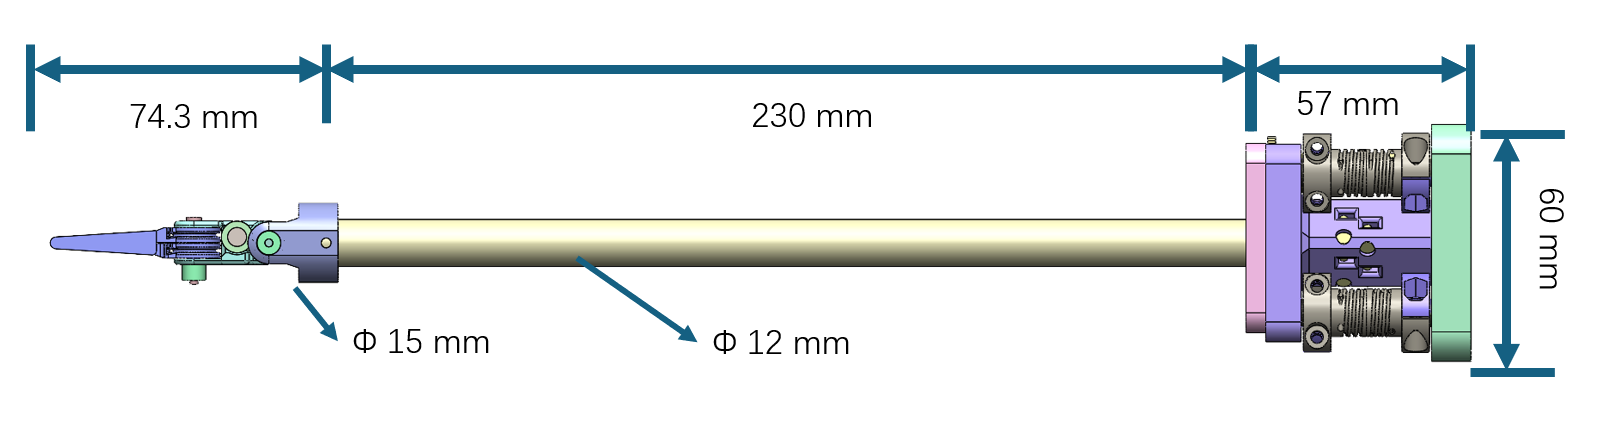
\includegraphics[width=\linewidth]{Figures/Chapter4/Winding_Size.png}
        \caption{Shaft and winding dimensions}
    \end{subfigure}

    \vspace{0.5em}

    \begin{subfigure}[b]{\linewidth}
        \centering
        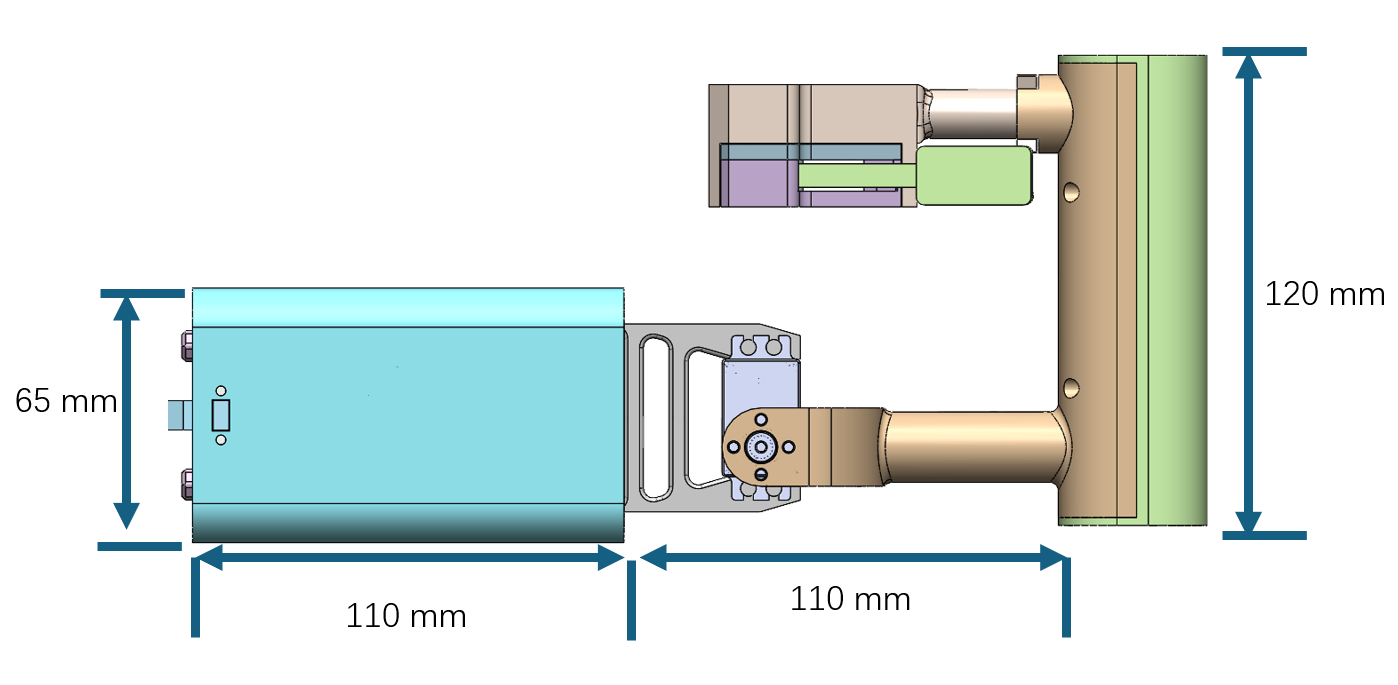
\includegraphics[width=\linewidth]{Figures/Chapter4/Main_Frame_Size.png}
        \caption{Main dimensions}
    \end{subfigure}
    \caption{Overall mechanical layout of the handheld tendon-driven instrument. The design separates the handheld actuation and control housing from the distal tool module so that the mass of motors and electronics is concentrated proximally, while the cable-driven tip remains compact.}
    \label{fig:main_frame_exploded}
\end{figure}

The system is organized into three physical modules: the proximal main frame, the cable-driven shaft and winding assembly, and the distal interchangeable tool. This modular arrangement follows the same proximal-actuation principle underlying the tendon-driven mechanism framework of this thesis, but adapts it to the stricter requirements of handheld surgical instrumentation. The main frame contains the higher-mass actuators, control board, and input interface; the shaft transmits cable tension through a guided internal route; and the distal tip converts cable displacement into multi-degree-of-freedom tool motion.

The total prototype mass is approximately 682\,g. Of this, the handheld body accounts for about 539\,g and the distal operating forceps account for about 143\,g. Concentrating most of the mass in the handle reduces the inertia of the distal portion and makes the device easier to orient during fine manipulation. The main frame measures approximately 110\,mm by 65\,mm in the motor housing region, while the distal shaft assembly uses a 250\,mm carbon tube with a 12\,mm outer diameter and a 15\,mm proximal coupling region. These dimensions were selected to balance compactness, cable routing clearance, and sufficient stiffness for hand-guided use.

\begin{table}[htbp]
    \centering
    \caption{Mass distribution of the handheld instrument prototype}
    \label{tab:mass_distribution}
    \begin{tabular}{p{0.23\linewidth} c p{0.48\linewidth}}
        \toprule
        Module & Mass & Design implication \\
        \midrule
        Handheld body & 539\,g & Motors, electronics, input interface, and main housing \\
        Operating forceps & 143\,g & Distal tool and shaft kept lighter to reduce manipulation inertia \\
        Total prototype & 682\,g & Bench-top handheld validation platform \\
        \bottomrule
    \end{tabular}
\end{table}

\subsection{Output Motors}
A key challenge for handheld cable-driven devices is selecting actuators that combine low mass with sufficient torque. The chosen output actuator, the Feetech STS3032 smart servo, offers a favorable torque-to-volume ratio and built-in low-level drive electronics useful for closed-loop control. It weighs approximately 20.6\,g, measures $23 \times 12 \times 27.5\,\mathrm{mm}$, and provides a stall torque of about $4.5\,\mathrm{kg\,cm}$, enabling reliable tensioning through small-diameter pulleys.

The four STS3032 servos are assigned to the output-side tool motions, including roll, pitch, yaw, and gripper opening/closing. Their serial-bus communication simplifies wiring and supports daisy-chaining, which reduces the number of conductors inside the handle and aids miniaturization. As smart servos, they can be commanded at the level of position and speed while also reporting state variables such as position, speed, load, voltage, temperature, and current. This low-level feedback allows the controller to implement repeatable position commands, monitor loading, and protect the cable drive from excessive tension.
\subsection{Input Motors and Sensors}

The control philosophy for this cable-driven handheld device is based on replicating the user's hand movements with high fidelity and translating them into precise motions of the distal end-effector. This requires a sophisticated input system that can accurately capture the intent of the user's fingers while providing sufficient force feedback and stability.


\begin{figure}[htbp]
    \centering
    \begin{subfigure}[b]{0.45\linewidth}
        \centering
        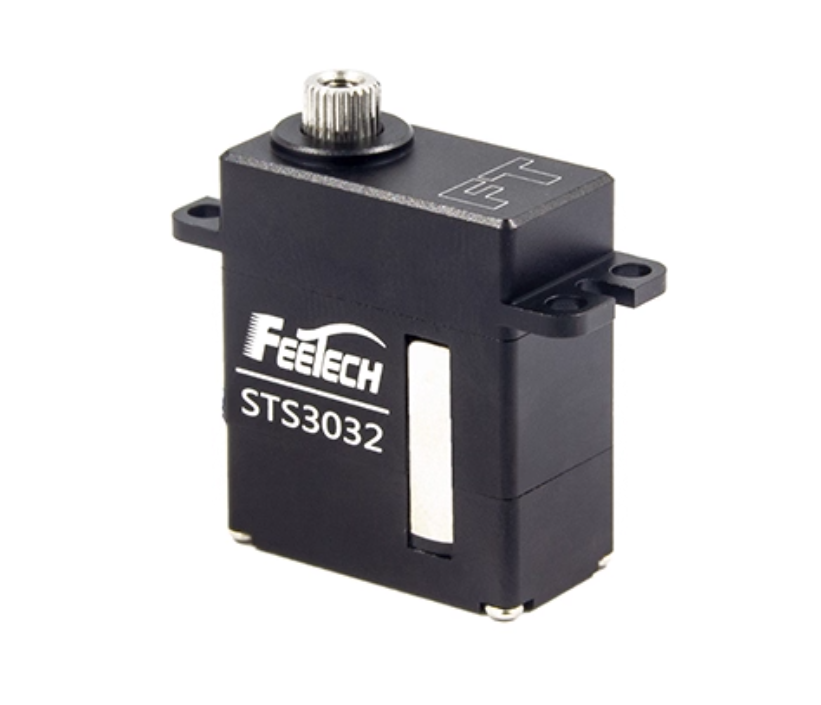
\includegraphics[width=\linewidth]{Figures/STS3032.png}
        \caption{Feetech 3032 for output}
        \label{fig:81}
    \end{subfigure}
    \hfill  % 水平填充，使两张图之间有空隙
    \begin{subfigure}[b]{0.45\linewidth}
        \centering
        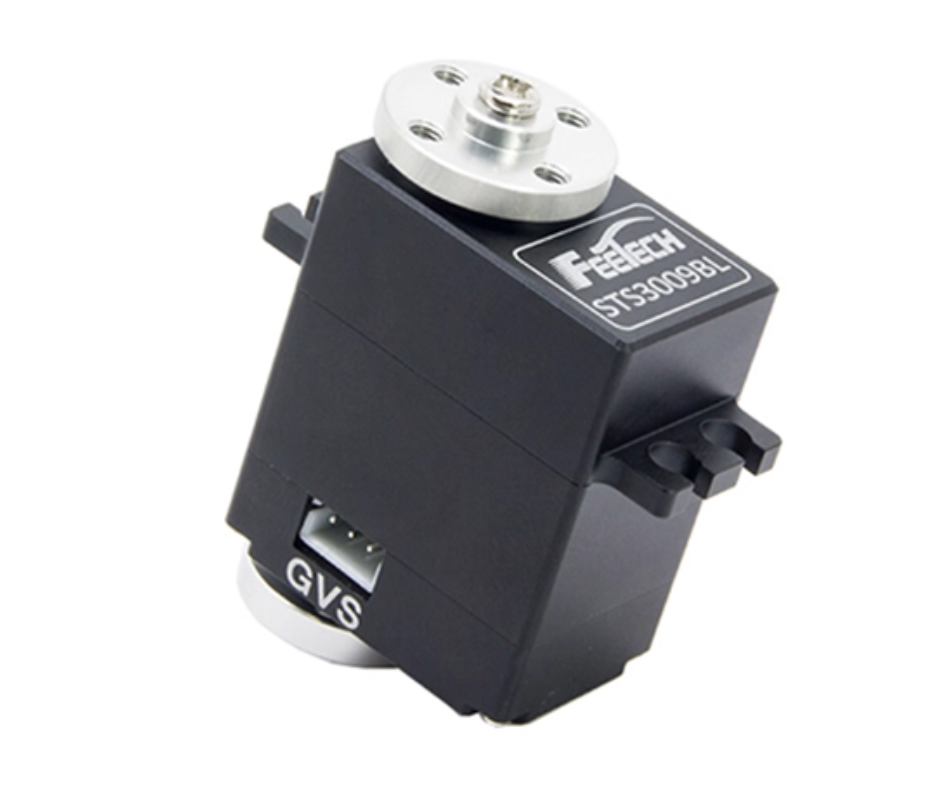
\includegraphics[width=\linewidth]{Figures/STS3009.png}
        \caption{Feetech 3009 for wrist inputs}
        \label{fig:82}
    \end{subfigure}
    \caption{Feetech servos: left motor for output (STS3032), right motor for wrist inputs (STS3009)}
\end{figure}

For the input actuation, shown in Fig.\ref{fig:81}, the Feetech STS3009 servo was selected based on a different set of requirements. Weighing approximately 45\,g, measuring $20 \times 30 \times 36.5\,\mathrm{mm}$, and providing a stall torque of about $11.5\,\mathrm{kg\,cm}$ ($\approx 1.13\,\mathrm{N\,m}$), this larger motor serves two essential functions in the input stage: it maintains mechanical equilibrium by resisting forces from the output tendons, thus offering a stable and responsive feel to the operator, and it helps filter out high-frequency physiological tremors or unintended jerks, ensuring that only deliberate commands are transmitted to the end-effector.


However, since the two input motors alone cannot fully capture all nuanced finger movements, a hybrid sensing strategy was implemented. The two STS3009 servos correspond to the input-side pitch and yaw axes. Two AMS AS5600 magnetic rotary encoders were integrated into the input mechanism to directly detect the remaining roll and open/close commands. These sensors provide 12-bit contactless angular sensing, enabling precise recognition of the pinching gesture of the index finger and thumb, which controls grasping, and the rotational movement of the fingers, which is translated into in-plane rotation of the end-effector. This combination of robust actuation and high-resolution sensing creates an intuitive and stable human-machine interface suitable for delicate manipulation tasks.

\begin{table}[htbp]
    \centering
    \caption{Actuator and sensor allocation in the handheld instrument}
    \label{tab:actuator_allocation}
    \small
    \setlength{\tabcolsep}{3pt}
    \begin{tabular}{@{}p{0.21\linewidth} p{0.09\linewidth} p{0.10\linewidth} p{0.16\linewidth} p{0.34\linewidth}@{}}
        \toprule
        Component & Quantity & Mass & Stall torque & Assigned function \\
        \midrule
        Feetech STS3032 & 4 & 20.6\,g & $4.5\,\mathrm{kg\,cm}$ & Output-side roll, pitch, yaw, and open/close control \\
        Feetech STS3009 & 2 & 45\,g & $11.5\,\mathrm{kg\,cm}$ & Input-side pitch and yaw sensing/stabilization \\
        AS5600 encoder & 2 & -- & -- & Input-side roll and open/close sensing \\
        \bottomrule
    \end{tabular}
\end{table}

\section{Cable Routing and Guidance System}
\subsection{Tip Design}
\begin{figure}[htbp]
    \centering
    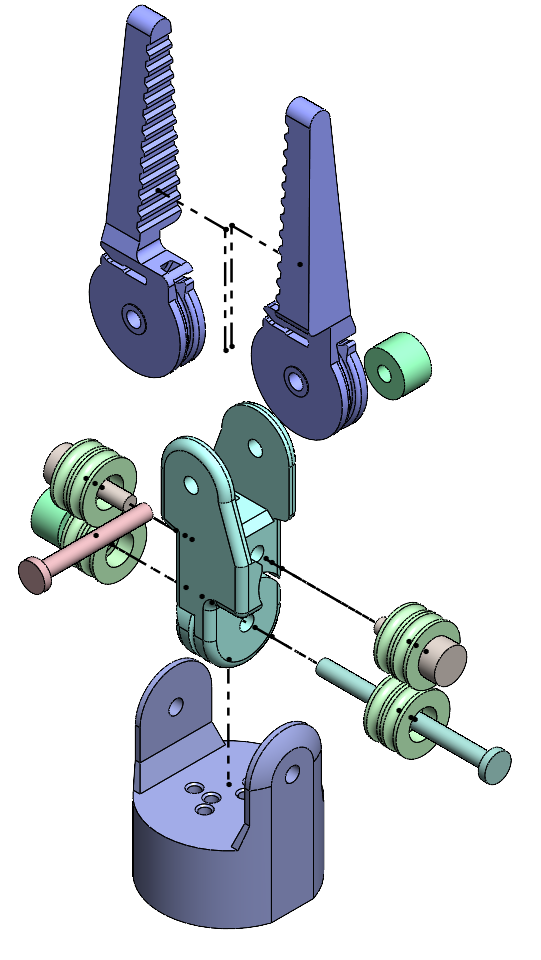
\includegraphics[width=0.5\linewidth]{Figures/Chapter4/Tip_Explode_View_Isometric.png}
    \caption{Exploded view of the distal tip assembly, including the jaw components, middle base, guide pulleys, pivot shafts, and base housing.}
    \label{fig:tip_exploded}
\end{figure}
In addition to motor performance, the accuracy and repeatability of the end-effector's motion are highly dependent on precise cable guidance and sustained tension control. To ensure consistent behavior during operation, each cable must be constrained to move freely yet securely within a meticulously designed path, minimizing unwanted friction and slack.

A specialized tip assembly has been developed to fulfill these requirements. As shown in Fig.~\ref{fig:tip_exploded}, the four cables are routed through custom-machined channels and pulley-like guides before terminating at the moving jaw components. These channels ensure that the cables remain aligned throughout the entire range of motion, avoiding cross-interference and reducing wear.

The two jaw components (fabricated in blue) are mounted onto a central middle base (green). To further enhance cable stability and minimize friction, donut-shaped guides machined via CNC (light green) are integrated into the middle base. These guides act as low-friction directional pulleys, maintaining cable position with high precision and reducing bending stress, thereby extending cable service life.

The main base housing (deep blue) is designed with precision-aligned holes that direct the cables perpendicularly toward the motors. This alignment is critical for maximizing force transmission efficiency and eliminating off-axis loading, which can introduce positioning errors and reduce system responsiveness.

The selected cable is a 7$\times$37 tungsten wire cable with a diameter of 0.5\,mm. It consists of seven braided strands, each composed of 37 fine wires, giving the cable sufficient flexibility for small-radius routing while maintaining a rated breaking force of 501.7\,N. The working cable length is approximately 350\,mm and is constrained by the current winding assembly, which uses a 250\,mm carbon tube as the main shaft structure. A Teflon guide tube is placed inside the carbon tube to reduce sliding friction and prevent metal-to-carbon abrasion. At the distal tip, integrated pulleys guide the cable around direction changes and reduce localized bending stress.

Through this integrated approach--combining dedicated guiding channels, pulley-supported direction changes, and perpendicular alignment--the system achieves high repeatability, reduced hysteresis, and smoother force transmission, making it suitable for delicate manipulation tasks requiring fine motor control.

\subsubsection{Finite Element Analysis of Tip Components}
\label{sec:tip_fea}
To validate the structural integrity of the distal tool assembly, finite element analysis (FEA) simulations were conducted on the two primary load-bearing components: the jaw/tip component and the middle base. The analysis used 6061-T4 aluminum alloy with an elastic modulus of $69{,}000\,\mathrm{N/mm^2}$, Poisson's ratio of 0.33, and a yield strength of $227.53\,\mathrm{N/mm^2}$. The global mesh size was set to 1.5\,mm, and local mesh control of 0.5\,mm was applied near the load and contact regions to better resolve stress concentrations around the cable-contact and pivot features.

The applied loads were derived from the STS3032 stall torque and therefore represent conservative worst-case loading rather than continuous normal operation. In normal use, firmware-level position, speed, and load limits prevent sustained stall operation; nevertheless, checking the components against a stall-torque-derived case provides a useful structural upper bound for the prototype.

\begin{figure}[htbp]
    \centering
    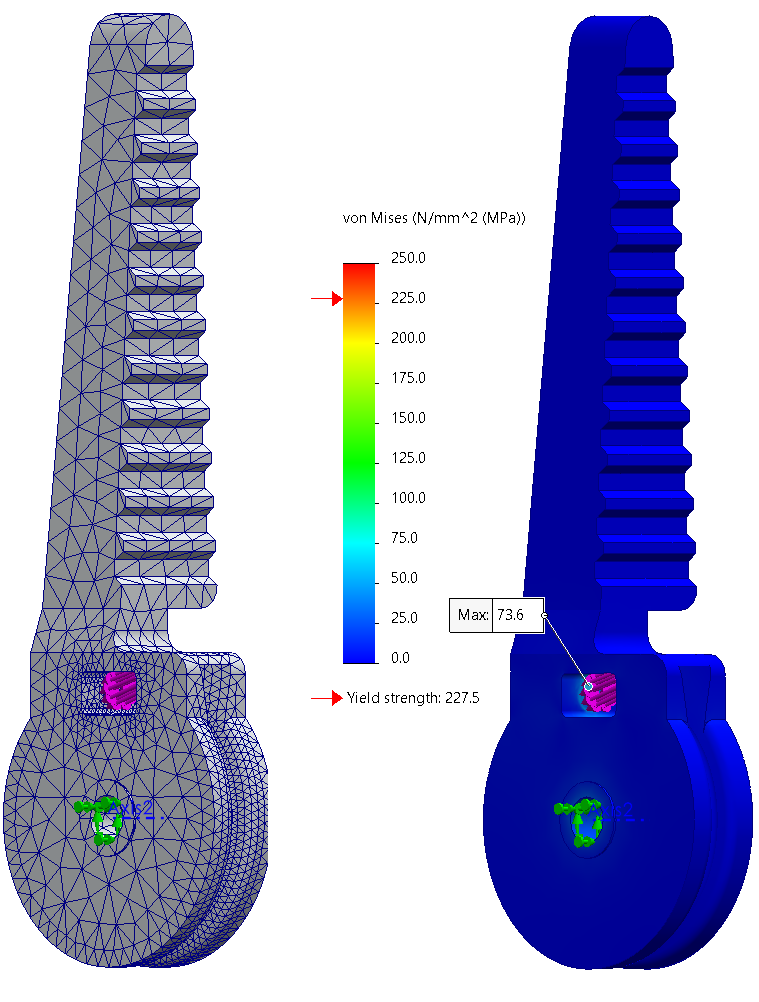
\includegraphics[width=0.7\linewidth]{Figures/Chapter4/Tip_Mesh_FEA.png}   
    \caption{FEA setup and von Mises stress result for the jaw/tip component under the stall-torque-derived loading condition.}
    \label{fig:tip_fea_new}
\end{figure}

\paragraph{Jaw/tip FEA}
The jaw/tip component was constrained at the pivot region and loaded at the cable-contact region according to the worst-case cable tension estimated from the STS3032 stall torque. The maximum von Mises stress was $73.6\,\mathrm{MPa}$, as shown in Fig.~\ref{fig:tip_fea_new}. Compared with the 6061-T4 yield strength of $227.53\,\mathrm{MPa}$, the corresponding safety factor is approximately
\[
SF_{tip}=\frac{227.53}{73.6}\approx 3.09 .
\]
This indicates that the jaw/tip component remains below yield under the conservative load case.

\begin{figure}[htbp]
    \centering
    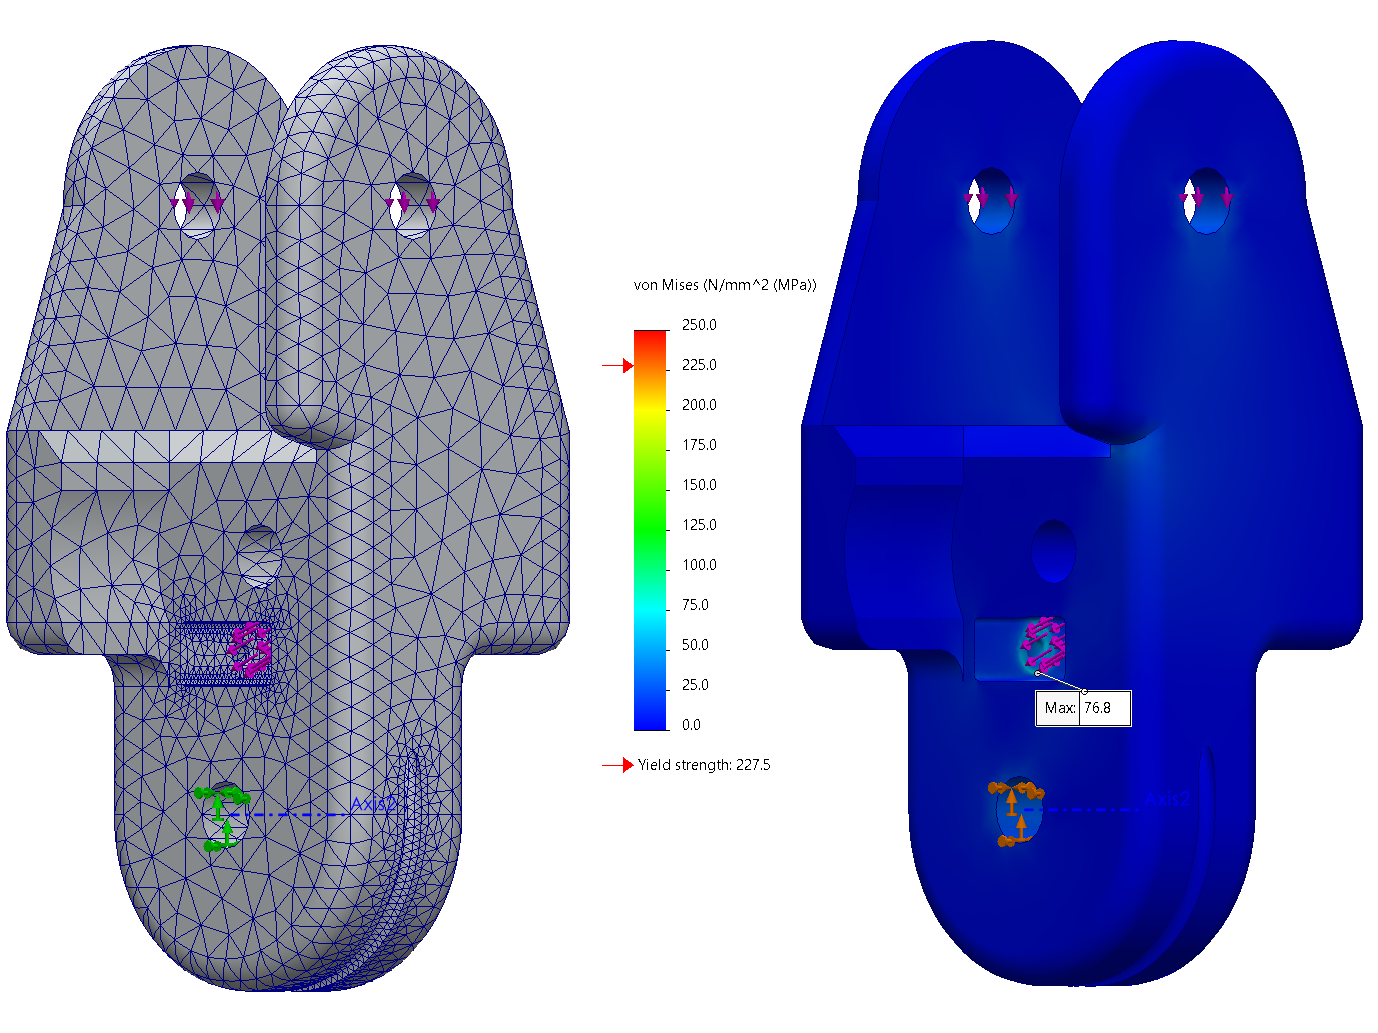
\includegraphics[width=0.9\linewidth]{Figures/Chapter4/Mid mesh&FEA.png}
    \caption{FEA setup and von Mises stress result for the middle base. The load case includes the cable-induced load and the extreme double downward forces transmitted from the tip.}
    \label{fig:mid_fea_new}
\end{figure}

\paragraph{Middle base FEA}
The middle base was evaluated under a combined loading case. In addition to the cable-induced load, the model includes the extreme double downward forces transmitted from the two tip/jaw components, representing a conservative condition in which both jaws transfer load into the base simultaneously. The maximum von Mises stress was $76.8\,\mathrm{MPa}$, as shown in Fig.~\ref{fig:mid_fea_new}. The corresponding safety factor is
\[
SF_{mid}=\frac{227.53}{76.8}\approx 2.96 .
\]
The result confirms that the middle base also remains below the yield strength under the combined extreme loading condition.

Overall, the updated FEA results indicate that both the jaw/tip and middle-base components have sufficient static strength for prototype validation under the conservative stall-torque-derived loading cases. The highest stresses appear near load introduction and geometric transition regions, so future design iterations should continue to use local fillets, adequate wall thickness around guide features, and careful deburring to reduce stress concentration and cable wear.
\subsection{Reel}

A fundamental challenge in cable-driven mechanisms lies in maintaining adequate tension during both winding and unwinding phases. In a conventional single-motor-single-cable configuration, unidirectional actuation presents a significant limitation: while rotation in one direction (e.g., clockwise) effectively pulls and tensions the cable, reverse rotation (counterclockwise) does not positively push the cable but often results in slack accumulation along the path. This leads to unpredictable response, reduced positional accuracy, and potential entanglement.

To address this issue, a paired-cable design has been implemented. The two cables corresponding to a single degree of freedom are affixed to the same axial shaft driven by one motor. This configuration effectively reforms the two independent cables into a continuous loop—functioning conceptually as a flexible drive belt. As a result, when the motor rotates in one direction, one cable is pulled while the other is simultaneously recovered, enabling bidirectional force transmission without slack accumulation.

\begin{figure}[htbp]
    \centering
  
    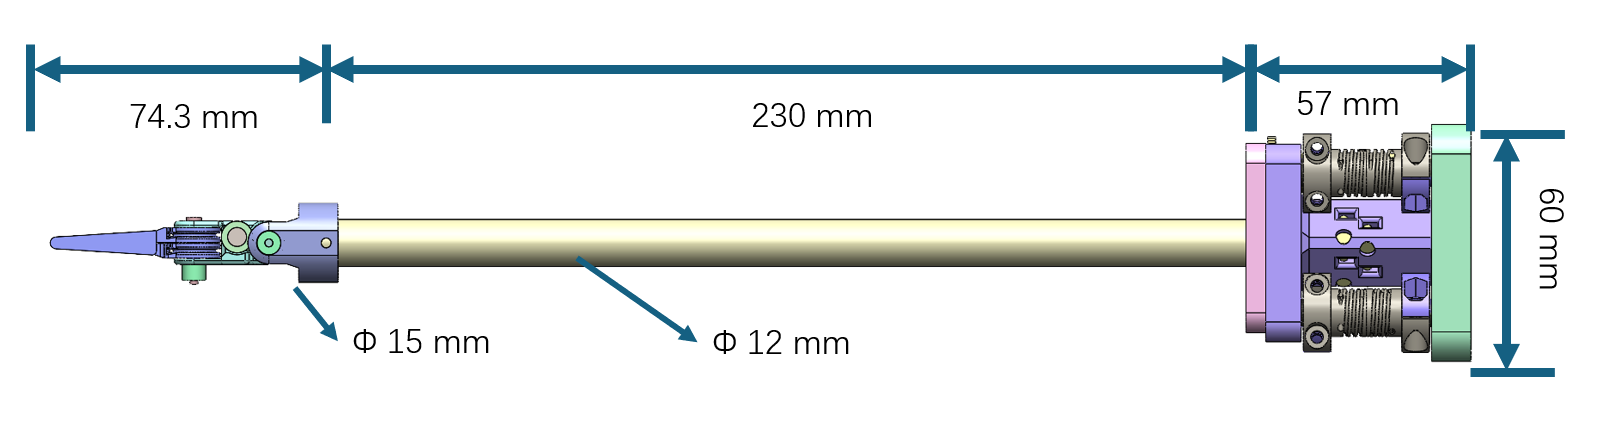
\includegraphics[width=\linewidth]{Figures/Chapter4/Winding_Size.png}

    \caption{Winding mechanism and shaft layout. The 250\,mm carbon tube provides the main shaft structure, while internal Teflon guidance and paired reel components maintain the cable route and tension.}
    \label{fig:winding_exploded}
\end{figure}

The key to ensuring effective operation of this belt-like linkage is sustained cable tension. To achieve this, the reel assembly is split into two distinct components, each dedicated to one cable. These two reel pieces are mounted on the same shaft and are designed to rotate in opposite directions relative to each other. This counter-rotation ensures that one cable is wound while the other is unwound during actuation, maintaining constant tension across the system.

To prevent slippage and undesired loosening of the cables during operation, one-way bearings are incorporated into the reel mechanism. As the name implies, these bearings permit free rotation in one direction while locking in the opposite direction. This feature is critical for preserving tension integrity, especially during transitions in motor direction or under varying load conditions. The use of one-way bearings enhances system reliability, improves motion accuracy, and minimizes the need for manual tension adjustments.

The reel diameter is matched to the tip rotation-axis diameter at 11\,mm, producing a nominal 1:1 displacement relationship between reel rotation and the corresponding tip-side cable displacement. This geometric matching simplifies command mapping because the controller does not need to compensate for an additional reel-to-tip radius ratio. For the roll transmission at the tip, the driving gear has 35 teeth and the driven gear has 65 teeth. The resulting angular reduction is $35/65$, while the ideal torque is increased by approximately $65/35$ before frictional losses. This ratio was selected to improve fine angular resolution and keep the quick-swap distal module compact.

\subsubsection{Actuator-to-Cable Force Mapping}
The reel geometry provides a direct way to estimate the upper-bound cable load generated by the output servos. The STS3032 stall torque is specified as approximately $4.5\,\mathrm{kg\,cm}$. Converting this value into SI units gives
\[
\tau_{stall}=4.5 \times 9.80665 \times 10^{-2}
\approx 0.441\,\mathrm{N\,m}
=441\,\mathrm{N\,mm}.
\]
With the reel diameter set to 11\,mm, the nominal reel radius is $r=5.5\,\mathrm{mm}$. Neglecting friction and cable compliance, the maximum single-cable tension that can be produced at the reel is therefore
\[
F_{cable,max}=\frac{\tau_{stall}}{r}
=\frac{441}{5.5}
\approx 80.2\,\mathrm{N}.
\]
This value is not intended to represent the normal continuous operating tension. It is an upper-bound estimate used for structural checking and safety-limit reasoning. In normal operation, the firmware commands position and speed within a limited range and avoids sustained stall conditions. Nevertheless, the stall-torque-derived load is useful because it defines the most severe actuator-driven load that the distal parts may experience before controller intervention.

The selected 0.5\,mm 7$\times$37 tungsten cable has a rated breaking force of 501.7\,N. Comparing this rating with the ideal stall-derived cable tension gives a cable-side strength margin of approximately
\[
SF_{cable}=\frac{501.7}{80.2}\approx 6.26 .
\]
This margin is evaluated only against axial cable breaking strength. It does not include losses from bending fatigue, local abrasion, knotting or crimp termination, pulley groove quality, or repeated sterilization and cleaning processes. For this reason, the cable is treated as structurally sufficient for prototype validation, but future versions should still include cycle-life tests under representative routing and tension profiles.

In addition to the axial strength margin, extra cable length was reserved for assembly and pretensioning. The prototype keeps approximately two additional turns on the 11\,mm-diameter reel, corresponding to an installation allowance of
\[
l_{allowance}=2\pi D=2\pi(11)\approx 69.1\,\mathrm{mm}.
\]
This reserved length is used to mount the cable securely and to tighten the opposing reel during setup. It should be interpreted as an installation and pretensioning allowance, not as an additional mechanical strength safety factor. The axial safety factor above describes the cable's load capacity under the stall-torque-derived tension, whereas the two-turn allowance improves assembly robustness and makes it easier to remove slack from the antagonistic cable pair.

\begin{table}[htbp]
    \centering
    \caption{Nominal actuator-to-cable force estimates for the output drive}
    \label{tab:actuator_cable_force}
    \small
    \setlength{\tabcolsep}{4pt}
    \begin{tabular}{@{}p{0.22\linewidth} p{0.22\linewidth} p{0.46\linewidth}@{}}
        \toprule
        Quantity & Value & Interpretation \\
        \midrule
        STS3032 stall torque & $4.5\,\mathrm{kg\,cm}$ & Maximum actuator torque before controller derating or protection \\
        Reel diameter & $11\,\mathrm{mm}$ & Matches the tip rotation-axis diameter for a nominal 1:1 displacement relationship \\
        Ideal maximum cable tension & $80.2\,\mathrm{N}$ & Upper-bound tension from stall torque and 5.5\,mm reel radius \\
        Tungsten cable breaking force & $501.7\,\mathrm{N}$ & Axial rating of the selected 0.5\,mm 7$\times$37 cable \\
        Cable axial safety margin & $6.26$ & Margin against ideal stall-derived cable tension before routing and termination effects \\
        Installation allowance & $\approx69.1\,\mathrm{mm}$ & Two reserved turns on the 11\,mm reel for mounting and opposing-reel pretensioning \\
        \bottomrule
    \end{tabular}
\end{table}

The same calculation also explains why the FEA load cases were derived from the actuator torque rather than from an arbitrary external force. The servo defines the largest force that the cable transmission can inject into the distal mechanism under normal electrical power. Because the reel and tip share the same nominal diameter, the cable displacement at the reel can be interpreted directly as cable displacement at the tip before friction and elastic stretch are considered. This makes the structural model traceable from motor specification to cable tension and then to local component loading.

For the roll transmission, the 35-tooth driving gear and 65-tooth driven gear modify the angular and torque relationship. Ideally, the output roll angle is
\[
\theta_{roll,out}=\frac{35}{65}\theta_{roll,in},
\]
while the torque available at the driven gear is increased by the inverse ratio,
\[
\tau_{roll,out}\approx \frac{65}{35}\tau_{roll,in}.
\]
This reduction is useful for handheld manipulation because the roll axis benefits from fine angular resolution and stable holding behavior. The penalty is that the input motor must rotate through a larger angular range to generate the same distal roll angle. Since the STS-series servos can be commanded precisely in position and speed, this penalty is acceptable for the current prototype.

\subsubsection{Cable Displacement and Motion Resolution}
The matched reel and tip diameter also provides a simple displacement model. For a reel radius $r$, a motor rotation of $\Delta\theta$ produces an ideal cable displacement
\[
\Delta l = r\Delta\theta,
\]
where $\Delta\theta$ is expressed in radians. With $r=5.5\,\mathrm{mm}$, one degree of servo rotation corresponds to
\[
\Delta l_{1^\circ}=5.5\frac{\pi}{180}
\approx 0.096\,\mathrm{mm}.
\]
This sub-0.1\,mm nominal cable-displacement increment is sufficient for fine command mapping at the prototype level. Actual distal motion resolution will be lower because of cable stretch, guide friction, backlash in the reel assembly, gear clearance, and servo quantization. However, the geometric relationship provides a useful baseline for firmware scaling and calibration.

In the paired-cable arrangement, each controlled degree of freedom can be represented by an antagonistic displacement pair:
\[
\Delta l_+ = r\Delta\theta,\qquad
\Delta l_- = -r\Delta\theta .
\]
The first cable is shortened while the second cable is recovered by the same nominal amount. This pairing is the reason the mechanism can transmit motion bidirectionally even though a cable can only carry tensile load. The design objective is not to keep the individual cable lengths fixed, but to keep their sum and pretension within a useful range:
\[
l_+ + l_- \approx constant,\qquad
T_{min}<T_+,T_-<T_{max}.
\]
Here $T_{min}$ is the minimum tension required to avoid slack and delayed response, while $T_{max}$ is the maximum safe tension set by the cable, distal components, actuator load, and target tissue or object.

\begin{table}[htbp]
    \centering
    \caption{Transmission relationships used for control interpretation}
    \label{tab:transmission_relationships}
    \small
    \setlength{\tabcolsep}{4pt}
    \begin{tabular}{@{}p{0.24\linewidth} p{0.20\linewidth} p{0.48\linewidth}@{}}
        \toprule
        Relationship & Expression & Design meaning \\
        \midrule
        Cable displacement & $\Delta l=r\Delta\theta$ & Converts servo rotation into linear tendon motion \\
        One-degree increment & $\Delta l_{1^\circ}\approx0.096\,\mathrm{mm}$ & Baseline command resolution at the 11\,mm reel diameter \\
        Antagonistic pair & $\Delta l_+=-\Delta l_-$ & Maintains bidirectional actuation through paired cables \\
        Roll gear ratio & $\theta_{out}=35\theta_{in}/65$ & Improves roll resolution and holding torque \\
        Useful tension window & $T_{min}<T<T_{max}$ & Prevents both slack and overload \\
        \bottomrule
    \end{tabular}
\end{table}

This analysis is intentionally first-order. It does not attempt to model the full nonlinear friction and compliance of the cable path. Instead, it defines the nominal relationships used to choose hardware dimensions and firmware gains. More accurate compensation would require measuring cable tension and distal pose over repeated trajectories, then identifying hysteresis parameters for each cable route. That work is beyond the scope of the present prototype but follows naturally from the framework established here.

\subsection{Motor Arrangement and Quick-Swap Mechanism}

As previously discussed, the STS3032 servos are employed as the driving motors for the cable reels. In practical surgical scenarios, various end-effector tips are often required throughout a single procedure. To accommodate this need, a quick-swap system has been integrated into the design, allowing for rapid and secure tip replacement without compromising system integrity.

To achieve a compact form factor suitable for handheld operation, the four motors are arranged in a rotationally symmetric pattern within the main housing. This layout optimizes spatial efficiency while maintaining sufficient clearance for motor power and communication cables, thereby preventing interference and ensuring reliable connectivity.
\begin{figure}[htbp]
    \centering
    \begin{subfigure}[b]{0.7\linewidth}
        \centering
        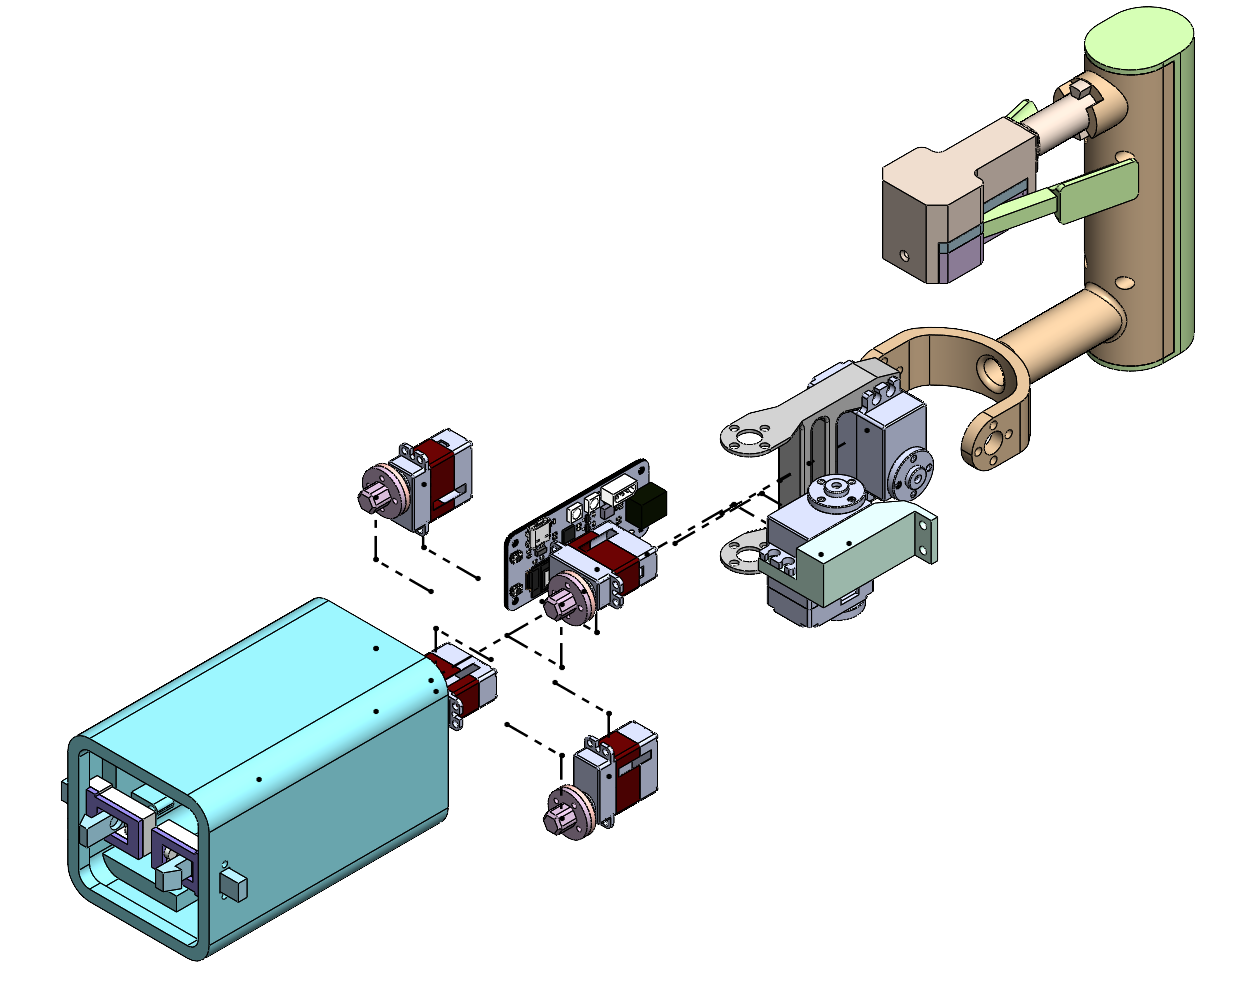
\includegraphics[width=\linewidth]{Figures/Chapter4/Main_Frame_ExplView_Iso.png}
        \caption{Exploded isometric view}
    \end{subfigure}

    \vspace{0.5em}

    \begin{subfigure}[b]{0.7\linewidth}
        \centering
        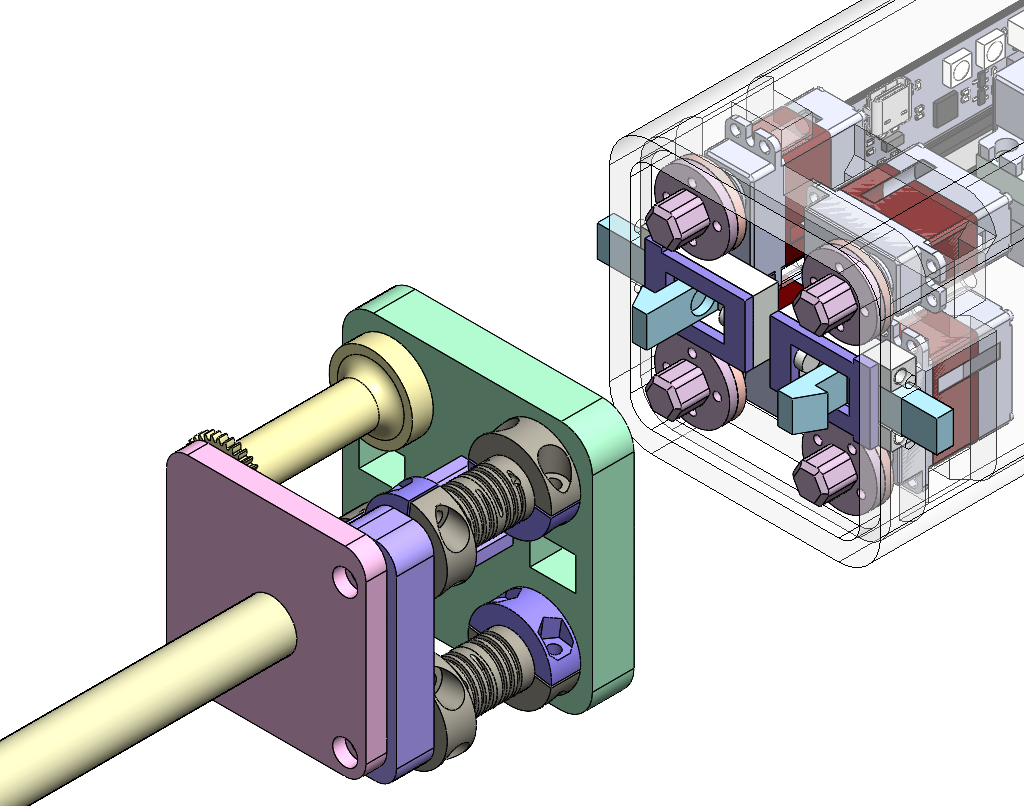
\includegraphics[width=\linewidth]{Figures/Motor Arrangement.png}
        \caption{Motor arrangement and quick-swap interface}
    \end{subfigure}
    
    \caption{Motor arrangement and quick-swap mechanism in the proximal frame. The output servos are packaged around the detachable shaft interface to preserve cable alignment while enabling tool exchange.}
    \label{fig:85}
\end{figure}
The quick-swap mechanism incorporates a user-friendly yet secure attachment scheme. Press-activated hooks are mounted within the main frame, enabling tool-free engagement and release. To attach a tip module, the user simply aligns and applies gentle pressure until the hooks audibly lock into place. For disengagement, bilateral release buttons must be depressed simultaneously while withdrawing the module. This dual-action release strategy prevents accidental detachment during operation, enhancing safety, while minimizing the number of steps required for module exchange.

This design ensures a robust mechanical and electrical connection during use, maintaining precise cable alignment and tension integrity while facilitating efficient tool interchange in time-sensitive surgical environments.

\subsection{Input Design}

The input module is designed to intuitively capture the user’s hand and finger motions with high precision and minimal latency. By integrating two STS3009 servos and two AS5600 magnetic encoders, the system is capable of sensing four degrees of freedom (DOFs): two DOFs from the wrist movement—yaw and pitch—and two DOFs from the fingers, namely roll and open/close actuation.

The wrist motions are translated through a dual-axis gimbal-like mechanism, where the STS3009 servos provide both actuation force and preliminary positional feedback. Fine rotational movements in yaw and pitch are accurately detected and relayed to the control system, enabling responsive and natural manipulation of the end-effector.
\begin{figure}[htbp]
    \centering
    \begin{subfigure}[b]{0.47\linewidth}
        \centering
        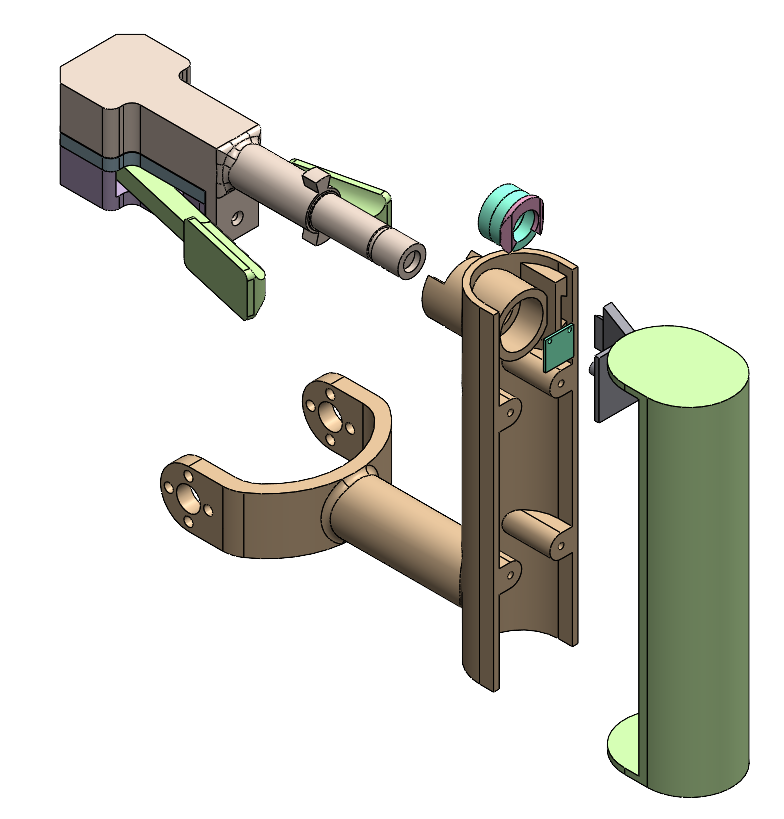
\includegraphics[width=\linewidth]{Figures/Chapter4/Input_Handle_ExplView_Iso.png}
        \caption{Input handle assembly}
    \end{subfigure}
    \hfill
    \begin{subfigure}[b]{0.47\linewidth}
        \centering
        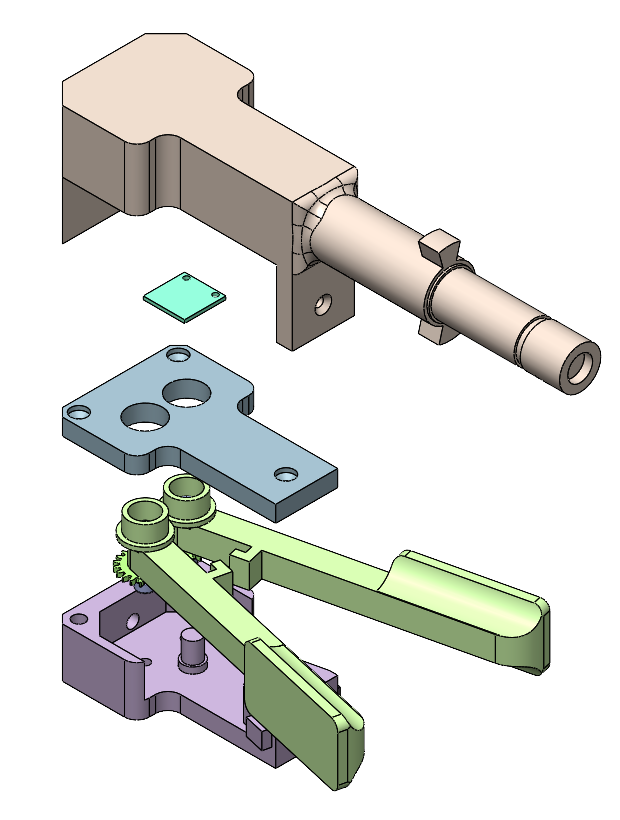
\includegraphics[width=\linewidth]{Figures/Chapter4/Pinch_ExplView_Iso.png}
        \caption{Pinch module}
    \end{subfigure}
    \caption{Input module design. Wrist pitch and yaw are captured through the STS3009-supported input handle, while roll and open/close commands are sensed by AS5600 encoders in the finger module.}
    \label{fig:86}
\end{figure}
Finger actions are captured using the high-resolution AS5600 encoders, which detect both the rolling gesture and the degree of opening or closing of the fingers. Specifically, the open/close mechanism is implemented as an interchangeable module, allowing customization based on user preference or task requirements. The lever length and rebound force can be easily adjusted or swapped, facilitating ergonomic adaptability and reducing user fatigue during prolonged operations.

This modular and sensor-rich input design ensures that the system can accommodate a wide range of hand sizes and operating styles while maintaining accurate and reliable motion mapping between the user and the instrument.

The project aims to implement a da Vinci–style surgical instrument claw effect using a compact 4-DOF hardware architecture: a 3-DOF manipulator arm plus a single gripper open/close degree of freedom. The system input is provided by the handle as three rotational joint angles and one gripper opening angle.

Since the manipulator itself has only three actual mechanical degrees of freedom, it cannot realize an arbitrary rotation axis in space. A specified direction in space requires three independent pose parameters, and a stable pose also consumes three degrees of freedom. This makes the system inherently over-constrained if arbitrary axis rotation is demanded. In contrast, the da Vinci system achieves effective 6-DOF stabilized control by using a larger arm to drive a smaller wristed arm in coordinated motion. Under the hardware constraints of this project, that six-degree-of-freedom stabilization strategy is not considered.

Instead, the control design adopts a decoupled attitude mapping. The coordinate system is defined using Euler angles to describe the desired end-effector orientation. The input attitude from the handle is mapped linearly to the output attitude of the manipulator, subject to the arm's three-degree-of-freedom limitations.


\subsection{Denavit–Hartenberg Coordinate Frames}
The coordinate frames are established using standard Denavit–Hartenberg conventions, as shown in Figures~\ref{fig:dhcord} and~\ref{fig:dhcord1}. The manipulator consists of three rotary joints, with the following D-H parameters:

\begin{table}[htbp]
    \centering
    \caption{Denavit–Hartenberg parameters for the 3-DoF manipulator}
    \label{tab:dhparams}
    \begin{tabular}{c c c c c l}
        \toprule
        Link & $\theta_i$ & $d_i$ & $a_i$ & $\alpha_i$ & Remarks \\
        \midrule
        1 & \(\theta_1\) & 0 & 0 & \(-90^\circ\) & Base rotation \\
        2 & \(90^\circ - \theta_2\) & 0 & \(-a_2\) & \(90^\circ\) & Upper arm rotation \\
        3 & \(\theta_3 - 180^\circ\) & 0 & \(a_3\) & 0 &  \\
        \bottomrule
    \end{tabular}
\end{table}

The following rotation matrix describes the end-effector orientation:

\[
A_1 =
\begin{bmatrix}
c_1 & 0 & -s_1 & 0 \\
s_1 & 0 & c_1 & 0 \\
0 & -1 & 0 & 0 \\
0 & 0 & 0 & 1
\end{bmatrix},
\]

\[
A_2 =
\begin{bmatrix}
s_2 & 0 & c_2 & -a_2 s_2 \\
c_2 & 0 & -s_2 & -a_2 c_2 \\
0 & 1 & 0 & 0 \\
0 & 0 & 0 & 1
\end{bmatrix},
\]

\[
A_3 =
\begin{bmatrix}
-c_3 & -s_3 & 0 & -a_3 c_3 \\
s_3 & -c_3 & 0 & a_3 s_3 \\
0 & 0 & 1 & 0 \\
0 & 0 & 0 & 1
\end{bmatrix}
\]
The end-effector pose is governed by the following equations:
\begin{align*}
P_x &= c_1 s_2(-a_3 c_3) + (-s_1)(a_3 s_3) + c_1 c_2(0) + (-a_2 c_1 s_2) \\
& \rightarrow P_x= -a_3 c_1 s_2 c_3 - a_3 s_1 s_3 - a_2 c_1 s_2 \\
P_y &= s_1 s_2(-a_3 c_3) + c_1(a_3 s_3) + s_1 c_2(0) + (-a_2 s_1 s_2) \\
& \rightarrow P_y= -a_3 s_1 s_2 c_3 + a_3 c_1 s_3 - a_2 s_1 s_2 \\
P_z &= -c_2(-a_3 c_3) + 0(a_3 s_3) + s_2(0) + a_2 c_2 \\
& \rightarrow P_z= a_3 c_2 c_3 + a_2 c_2
\end{align*}
The orientation of the end effector can also be expressed through the base axis direction vectors shown in Table~\ref{tab:axisdir}.

\begin{table}[htbp]
\centering
\caption{End-effector base-axis direction vectors}
\label{tab:axisdir}
\begin{tabular}{|l|l|l|l|}
\hline
\textbf{Direction} & \textbf{X-axis  ($n$)} & \textbf{Y-axis  ($o$)} & \textbf{Z-axis  ($a$)} \\
\hline
Base X-axis & $-c_1 s_2 c_3 - s_1 s_3$ & $-c_1 s_2 s_3 + s_1 c_3$ & $c_1 c_2$ \\
\hline
Base Y-axis & $-s_1 s_2 c_3 + c_1 s_3$ & $-s_1 s_2 s_3 - c_1 c_3$ & $s_1 c_2$ \\
\hline
Base Z-axis & $c_2 c_3$ & $c_2 s_3$ & $s_2$ \\
\hline
\end{tabular}
\end{table}

\begin{figure}[htbp]
    \centering
    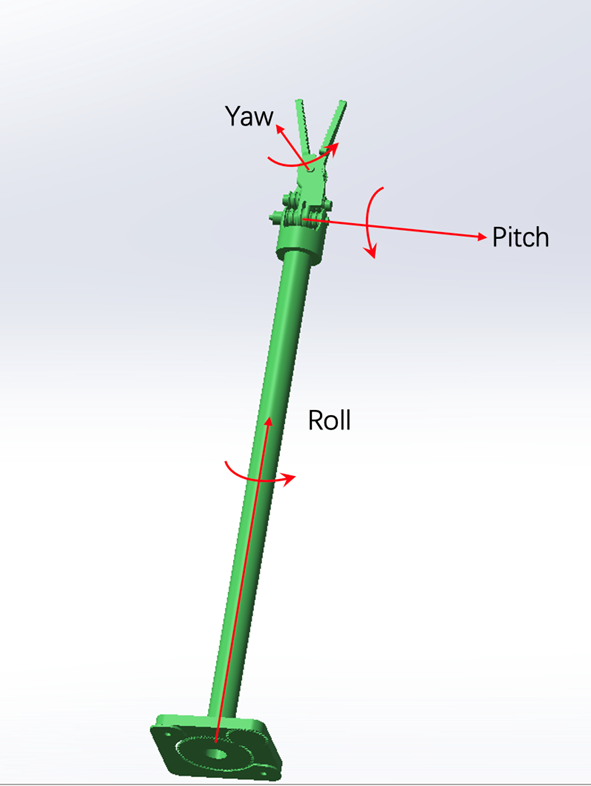
\includegraphics[width=0.7\linewidth]{Figures/DH cord1.png}
    \caption{Denavit–Hartenberg coordinate frame definition for the manipulator}
    \label{fig:dhcord}
\end{figure}

\begin{figure}[htbp]
    \centering
    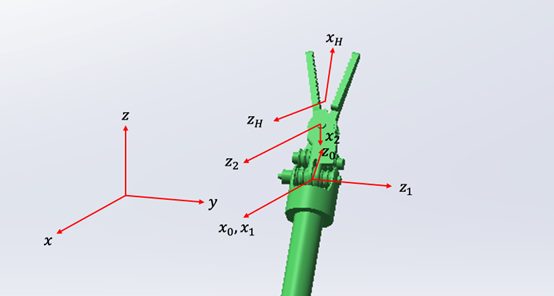
\includegraphics[width=0.8\linewidth]{Figures/DH cord.png}
    \caption{Alternative view of the D-H coordinate frames and joint axes}
    \label{fig:dhcord1}
\end{figure}

\subsection{System Architecture and Data Flow}
The control system is implemented on an ESP32 microcontroller running FreeRTOS, enabling real-time processing of sensor inputs and actuator commands. The architecture follows a cyclic loop structure, as illustrated in the firmware code, where sensor feedback is continuously acquired, processed, and translated into motor commands.

At the core of the system is a feedback loop that reads position, speed, load, voltage, temperature, and current from eight Feetech STS-series servos via UART communication. This multi-modal feedback provides the foundation for state estimation and control. The input module captures user intent through four degrees of freedom: wrist yaw, pitch, roll, and gripper opening/closing, using AS5600 magnetic encoders and STS3009 servos for precise motion detection.

The overall control pipeline is organized into four layers. The first layer is the sensing layer, where the AS5600 encoders and servo feedback registers are sampled. The second layer is the intent-estimation layer, where raw input angles are converted into centered, filtered, and range-limited user commands. The third layer is the command-mapping layer, where the desired roll, pitch, yaw, and open/close commands are transformed into individual output-servo setpoints. The fourth layer is the actuator layer, where the STS3032 servos execute the command while returning load and state information for monitoring.

\begin{table}[htbp]
    \centering
    \caption{Control-layer organization of the handheld instrument}
    \label{tab:control_layers}
    \begin{tabular}{p{0.22\linewidth} p{0.32\linewidth} p{0.30\linewidth}}
        \toprule
        Layer & Main function & Representative signals \\
        \midrule
        Sensing & Acquire raw input and actuator states & AS5600 angle, servo position, speed, load, voltage, temperature, current \\
        Intent estimation & Center, scale, filter, and limit the user's motion & Roll, pitch, yaw, and gripper-opening commands \\
        Command mapping & Convert user commands into output-axis setpoints & Four STS3032 position targets and motion limits \\
        Actuation and monitoring & Execute commands and detect abnormal states & Servo enable/unload state, load threshold, communication status \\
        \bottomrule
    \end{tabular}
\end{table}

This layered structure is important because it separates user-interface behavior from distal tool behavior. The handle may be redesigned in future versions without changing the output transmission model, provided that it still supplies normalized roll, pitch, yaw, and open/close commands. Similarly, the distal tool can be replaced through the quick-swap interface as long as its cable routing and command scaling remain compatible with the actuator layer. This modularity supports the broader thesis goal of applying tendon-driven design principles across multiple mechanical embodiments.

\subsection{Intent Estimation and Command Mapping}
User inputs are mapped from encoder readings to angular commands. The firmware calculates roll, pitch, yaw, and gripper commands by scaling encoder positions relative to a midpoint. For instance, $roll_cmd$ is derived from the difference between encoder p8 and the midpoint, scaled to degrees. These commands are then transformed into servo-specific inputs, accounting for mechanical ratios and phase offsets to ensure coordinated motion.

The transformation incorporates kinematic considerations, such as the differential yaw control for the gripper jaws, where $s3\_yaw\_right$ and $s4\_yaw\_left$ are adjusted based on $yaw\_in$ and $gripper\_cmd$ to achieve symmetric or asymmetric grasping.

To robustly infer operator intent in the presence of noise and delay, an Extended Kalman Filter (EKF) can be integrated as a future enhancement. The EKF would fuse sensor inputs from AS5600 encoders, motor encoders, and optional inertial measurements from an IMU module. It maintains estimates of finger poses, wrist orientation, and cable tensions, enabling predictive control and improved stability during rapid transitions. This probabilistic approach handles uncertainties in sensor readings, providing smoother and more reliable command generation compared to the current direct mapping.

In the current prototype, the direct mapping can be written as a normalized affine transformation. For an input sensor reading $q_i$, the corresponding command is
\[
u_i = k_i(q_i-q_{i,0}),
\]
where $q_{i,0}$ is the neutral reference measured during homing and $k_i$ is the command gain selected for that degree of freedom. The command is then saturated:
\[
u_i^{sat}=\mathrm{clip}(u_i,u_{i,min},u_{i,max}).
\]
The saturation step is not only a software convenience. It is a safety mechanism that prevents the handle from commanding cable travel beyond the mechanically validated range of the reel, guide tube, pulley, and distal joint.

The four output commands are intentionally decoupled at the operator level:
\[
\mathbf{u}=
\begin{bmatrix}
u_{roll} & u_{pitch} & u_{yaw} & u_{grip}
\end{bmatrix}^T .
\]
They are then mapped into motor targets:
\[
\mathbf{m}=M\mathbf{u}+\mathbf{m}_0 ,
\]
where $\mathbf{m}$ contains the four STS3032 target positions, $M$ is a sign-and-scale matrix determined by cable routing direction and gear ratio, and $\mathbf{m}_0$ contains the neutral motor positions. In the simplest case, each row of $M$ contains only one dominant nonzero term. In practice, the jaw and yaw axes may be coupled because the same distal geometry contributes to both lateral orientation and symmetric jaw motion. The firmware therefore applies sign offsets so that symmetric closing commands move both jaws together, while yaw commands create differential motion.

\begin{table}[htbp]
    \centering
    \caption{Command interpretation for the four output degrees of freedom}
    \label{tab:command_mapping}
    \begin{tabular}{p{0.18\linewidth} p{0.24\linewidth} p{0.38\linewidth}}
        \toprule
        Command & Primary input source & Output interpretation \\
        \midrule
        Roll & AS5600 roll encoder & Rotates the distal tool through the 35:65 gear transmission \\
        Pitch & STS3009-supported wrist input & Bends the distal tool in the pitch plane through an antagonistic cable pair \\
        Yaw & STS3009-supported wrist input & Produces lateral distal orientation through differential cable motion \\
        Open/close & AS5600 pinch encoder & Controls jaw aperture and grasping tension \\
        \bottomrule
    \end{tabular}
\end{table}

Several practical issues arise in this mapping. First, the neutral position must be repeatable. If the user powers on the device while the handle is displaced, the controller may interpret a biased input as the center position. The startup routine therefore moves the servos to known neutral positions and records sensor baselines before enabling full output motion. Second, the command gain must be conservative enough to prevent sudden distal motion, especially near the limits of the jaw and pitch axes. Third, the sign convention must be verified physically after every cable rerouting or tip replacement, because crossing a cable or reversing a reel direction changes the relationship between motor rotation and distal motion.

\subsection{Low-Level Actuation and Tension Management}
Actuation is handled through direct position control of the STS3032 servos for the output stage and STS3009 for input stabilization. The code implements a locking mechanism for the gripper motors: when the gripper is open beyond a threshold $(gripper_open = 5.0 degrees)$, the motors are unloaded to reduce power consumption and allow free motion; otherwise, they are locked to maintain tension.

This tension management is critical for cable-driven systems, preventing slack while enabling compliant interaction. The firmware uses the servo's built-in position mode with zero speed and acceleration for precise control, ensuring smooth transitions without oscillations.

For a tendon-driven tool, low-level control cannot be evaluated only by whether the servo reaches a target position. The control objective is to reach the target while maintaining the cable inside a useful tension range. A simple practical interpretation is:
\[
T_{min}<T(t)<T_{max},
\]
where $T_{min}$ prevents backlash and delayed response, while $T_{max}$ prevents cable damage, component yielding, motor overheating, and excessive tool force. Because the current prototype does not include direct inline cable-load cells at every tendon, the firmware uses servo load feedback as an indirect monitoring signal. This indirect signal is sufficient for prototype protection and debugging, but it is not a substitute for calibrated distal force sensing.

The control strategy therefore combines position commands with state-dependent enable and unload logic. When the gripper is open beyond the defined threshold, the controller can unload selected servos to avoid unnecessary cable tension and heat generation. When the gripper is closing or holding, the output servos are enabled so that the cable path remains tensioned and the jaws do not drift. This behavior is particularly important for surgical-style use because an unintended holding force could damage tissue, while an unintended release could cause loss of object control.

\begin{table}[htbp]
    \centering
    \caption{Representative tension-management states}
    \label{tab:tension_management_states}
    \begin{tabular}{p{0.20\linewidth} p{0.33\linewidth} p{0.31\linewidth}}
        \toprule
        State & Controller behavior & Purpose \\
        \midrule
        Open and idle & Selected motors unloaded or low-torque holding & Reduce heat and avoid unnecessary distal force \\
        Commanded motion & Position targets updated with speed limits & Produce smooth motion while avoiding sudden cable loading \\
        Grasp or hold & Motors enabled and position maintained & Preserve cable tension and jaw closure \\
        Overload indication & Stop, relax, or reject further closing command & Protect cable, distal parts, and target object \\
        Communication fault & Stop command update and enter error indication & Prevent uncontrolled motion under missing feedback \\
        \bottomrule
    \end{tabular}
\end{table}

The one-way bearings in the reel assembly complement the firmware strategy. Mechanically, they reduce the tendency for a cable to unwind when load direction changes or when the motor is temporarily unloaded. Electrically, the firmware avoids repeatedly driving the motor against the same holding load when mechanical retention is sufficient. This mechanical-electrical division of responsibility is useful in a handheld device because it reduces power consumption and heat while improving perceived stability.

\subsection{System Implementation and Details}
Safety is ensured through conditional motor unloading and error management. When feedback faults occur—such as communication dropouts—the system illuminates an error LED and stops execution. At startup, a homing routine moves the servos to their neutral positions, enabling the encoders to establish reference baselines.

While running, the lock/release mechanism functions as a safety measure: it relieves cable tension whenever the gripper is open, preventing unintended forces on tissue.

Visual and diagnostic feedback is delivered through a WS2812 LED strip and serial output. Error conditions activate red LEDs, whereas normal operation leaves the indicators off. Both USB and Bluetooth connectivity support data logging, facilitating offline analysis of control performance and user interactions.

The firmware communicates with servos via HardwareSerial at 500k baud and uses standard Serial for debugging. Motor commands are assembled using a custom protocol that includes unload/enable directives. The main loop executes roughly every 3~ms, striking a balance between system responsiveness and computational overhead.

This implementation embodies a practical tendon-driven control framework, translating high-level intentions into low-level actuation while emphasizing safety and usability within a compact, real-time system.

\subsubsection{Homing and Calibration Procedure}
The homing procedure establishes the mechanical and electronic zero state of the instrument. At power-on, the controller first checks communication with all STS-series servos and verifies that the AS5600 encoders return valid angular readings. The output servos are then moved to their neutral positions, and the input sensors are sampled to define the operator-center reference. This sequence prevents the system from immediately converting an arbitrary startup posture into a distal tool command.

Calibration is especially important because the cable transmission is not perfectly rigid. Small changes in cable pretension, guide-tube seating, reel assembly position, and quick-swap module alignment can shift the neutral distal pose. The prototype therefore treats neutral calibration as part of the operating procedure rather than as a one-time factory setting. After the tool module is inserted, the user can bring the handle to its neutral posture and allow the firmware to store the corresponding encoder baselines. The output motors then apply only limited holding torque until the command state is enabled.

\begin{table}[htbp]
    \centering
    \caption{Startup and calibration sequence}
    \label{tab:startup_calibration}
    \begin{tabular}{p{0.16\linewidth} p{0.44\linewidth} p{0.24\linewidth}}
        \toprule
        Step & Operation & Failure response \\
        \midrule
        Device check & Confirm servo communication and sensor readings & Enter error indication if feedback is missing \\
        Mechanical neutral & Move output servos to predefined neutral positions & Keep motors unloaded if motion is blocked \\
        Input baseline & Record AS5600 and STS3009 neutral readings & Reject commands until readings are stable \\
        Pretension check & Apply limited holding command and inspect response & Relax cable if load estimate is abnormal \\
        Enable control & Accept user roll, pitch, yaw, and grip commands & Continue monitoring load and communication \\
        \bottomrule
    \end{tabular}
\end{table}

This procedure also supports the quick-swap concept. If a distal module is exchanged, the controller does not assume that the previous neutral offset remains valid. Recalibration after module insertion reduces the risk of accumulating cable bias across tool changes. In a future clinical version, this procedure would need to be further constrained by sterilizable connectors, keyed mechanical alignment, and automated verification of tool identity.

\subsubsection{Fault Handling and Safety State Machine}
The safety logic can be represented as a state machine that limits how the device reacts to abnormal conditions. The normal operating state accepts user commands and updates servo targets. If the input command exceeds the allowed range, the controller clips the command rather than passing it directly to the output servo. If the servo load or temperature rises beyond an acceptable range, the controller can stop further closing motion, relax the corresponding cable, or enter a fault state depending on severity. If communication with a servo is lost, the system stops command updates and provides a visible error indication through the LED interface.

\begin{table}[htbp]
    \centering
    \caption{Safety-related events and controller responses}
    \label{tab:safety_events}
    \begin{tabular}{p{0.26\linewidth} p{0.34\linewidth} p{0.24\linewidth}}
        \toprule
        Event & Detection source & Response \\
        \midrule
        Command exceeds travel limit & Scaled input command after saturation check & Clip command to validated range \\
        Possible cable overload & Servo load feedback or abnormal holding demand & Stop closing or relax affected axis \\
        Servo communication fault & Missing or invalid UART response & Freeze command update and show error LED \\
        Startup bias & Input baseline unstable during homing & Delay enabling output motion \\
        Excessive heating risk & Servo temperature or prolonged high-load state & Reduce holding command or unload motor \\
        Quick-swap uncertainty & Module exchange or alignment disturbance & Require neutral recalibration \\
        \bottomrule
    \end{tabular}
\end{table}

The safety state machine is deliberately conservative. The prototype is intended to validate mechanism feasibility, not to maximize speed at the expense of controllability. Therefore, ambiguous states are treated as reasons to stop or relax motion rather than to continue driving the tendon path. This approach is consistent with the design philosophy of cable-driven medical tools, where the consequences of excessive force are more severe than the inconvenience of stopping a command.

\subsubsection{Control Limitations}
The present control implementation has several limitations. First, distal pose is inferred from motor position and transmission geometry rather than measured directly at the tool tip. As a result, cable stretch, friction, backlash, and guide-tube movement can create differences between commanded and actual pose. Second, load monitoring is indirect. Servo load feedback is useful for detecting abnormal trends, but it does not provide a calibrated measurement of cable tension or tissue force. Third, the current mapping is mostly linear. This is appropriate for a first prototype, but the real transmission is nonlinear because friction changes with bend angle, direction of motion, and cable normal force.

These limitations define the next control-development path. A more advanced version should add distal pose or force sensing, identify hysteresis maps for each cable route, and compensate for cable stretch under load. Repeated cyclic tests should be used to measure backlash, settling time, and drift. The current architecture is compatible with these future improvements because it already separates sensing, intent estimation, command mapping, and low-level actuation. The missing elements are therefore additional measurement channels and experimentally identified compensation parameters rather than a complete redesign of the control framework.

\chapter{General Discussion}

\label{ChapterDiscussion}

\begin{chaptersummary}
This chapter synthesizes the two prototype studies presented in the thesis, with Lasso Gripper serving as the main mechanism contribution and the handheld surgical instrument serving as a complementary application case. Rather than treating the two systems as unrelated devices, the discussion identifies the common design variables that govern both systems: proximal actuation, flexible tensile transmission, routing geometry, tension management, compliance, sensing, and task-specific interaction geometry.

The chapter also evaluates what has and has not been demonstrated by the present work. Lasso Gripper is treated as the main mechanism contribution of the thesis, showing the feasibility of a free tensile loop for adaptive capture under uncertain object geometry. The handheld instrument is treated as a complementary application case, showing how guided cable transmission can be packaged into a compact, multi-DOF tool architecture. The discussion clarifies the limitations of qualitative demonstrations, static FEA, and open-loop control, and extracts practical design guidelines for future tendon-driven robotic systems.
\end{chaptersummary}

\section{Unifying View of the Two Prototype Systems}

The thesis develops two systems that appear different at the application level. Lasso Gripper is an adaptive robotic end-effector for capturing objects using a launched and retracted string loop. The handheld surgical instrument is a compact motorized laparoscopic tool that transmits motion from proximal actuators to a distal multi-DOF tip through guided cables. One system operates in an open manipulation environment and emphasizes capture tolerance; the other operates under medical-device constraints and emphasizes precision, packaging, and reliable bidirectional transmission. However, at the mechanism level, both systems address the same central question: how can flexible tensile elements be used to produce useful robotic behavior without allowing flexibility, slack, and hysteresis to dominate the system response?

This perspective is important for interpreting the thesis as a coherent body of work. The two prototypes are not intended to solve the same task, nor should their experimental results be compared directly as if they were alternative grippers. They are parallel embodiments under the same tendon-driven mechanism framework, but they do not carry equal roles in the thesis. Lasso Gripper is the primary mechanism platform and the main source of novelty; the surgical instrument is a complementary engineering case that examines the same design variables under tighter packaging and control constraints. Together, they occupy two ends of a design spectrum for tendon-driven mechanisms. Lasso Gripper uses a deliberately unconstrained loop. Its advantage arises from allowing the tensile element to occupy a large capture region and conform to objects with uncertain geometry. The surgical instrument uses a highly constrained cable path. Its advantage arises from imposing routing, guidance, and paired winding so that cable motion becomes repeatable enough for handheld teleoperation. The design problem is therefore not whether a cable should be free or constrained, but how much constraint should be introduced for the target task.

In Lasso Gripper, the loop is useful because it is not forced to behave like a rigid linkage. It can sweep across a region, tighten around protrusions or enclosed features, and distribute contact over a larger portion of the object surface. This is particularly valuable for deformable, oversized, or moving objects, where precise antipodal point placement is difficult. In the surgical instrument, by contrast, an unconstrained cable would be unacceptable. The cable must remain inside a guide path, maintain pretension, avoid crossing or entanglement, and transmit motion with predictable phase and displacement. The same physical property--flexible tension transmission--therefore supports two different functions depending on the surrounding mechanical constraints.

This relationship can be summarized through several mechanism-level variables. Both systems share the same underlying design concerns, but each system chooses a different point in the tendon-driven design space.

\begin{description}[style=nextline,leftmargin=1.5em,labelindent=0pt,itemsep=0.8em]
    \item[\textbf{Tensile element role.}]
    Lasso Gripper uses a free loop that creates an adaptive capture region. The handheld surgical instrument uses guided cables that transmit tool motion from proximal servos.

    \item[\textbf{Primary objective.}]
    Lasso Gripper aims to increase capture tolerance and distributed contact. The handheld instrument aims to preserve distal dexterity and repeatable control in a compact form factor.

    \item[\textbf{Routing constraint.}]
    Lasso Gripper imposes a low level of constraint, allowing the loop shape to remain task-dependent and partly self-supporting. The surgical instrument imposes a high level of constraint through guide tubes, pulleys, reels, and tip channels.

    \item[\textbf{Tension management.}]
    In Lasso Gripper, retraction tension closes and secures the loop. In the surgical instrument, paired-cable winding maintains bidirectional force transmission.

    \item[\textbf{Main uncertainty.}]
    Lasso Gripper is mainly affected by loop placement, object motion, and object geometry. The surgical instrument is mainly affected by cable stretch, friction, backlash, and user-command mapping.

    \item[\textbf{Validation evidence and limitation.}]
    Lasso Gripper is supported by representative grasping demonstrations and workspace analysis, but it remains demonstration-focused without large-sample statistics. The surgical instrument is supported by mechanical design, kinematic mapping, FEA, packaging, and control implementation, but it remains a prototype without clinical or long-duration reliability validation.
\end{description}

The shared mechanism framework also clarifies why both systems are relevant to the broader field of robotic manipulation. Rigid-link mechanisms are effective when the desired interaction geometry is known, the object is sufficiently rigid, and the workspace is accessible. Tendon-driven mechanisms become attractive when the designer wants to relocate actuation, reduce distal mass, introduce compliance, or create interaction regions larger than the physical end-effector. These advantages are not free. They require explicit design attention to routing, pretension, friction, sensing, and load paths. The thesis demonstrates this trade-off through a primary free-loop gripper and a secondary guided-cable instrument rather than through a single optimized final device.

\section{Tension as a Central Design Variable}

Tension is the most important internal state in both prototypes. In a rigid mechanism, joint position is often the primary variable used to reason about function. In a tendon-driven mechanism, position alone is insufficient. A cable can have the correct nominal displacement but still fail to transmit useful force if it is slack. Conversely, excessive tension can damage an object, overload a component, increase friction, or accelerate wear. The useful operating region is therefore bounded from below by the need to avoid slack and from above by safety, material strength, and task-specific contact limits.

For Lasso Gripper, tension controls the transition between loop formation, loop placement, tightening, and transport. During launch, the loop must retain enough shape to sweep across the target region. During retraction, tension must increase fast enough to close the loop before the object escapes, but not so aggressively that the string slips to an undesired location or damages a deformable object. During lifting, tension must remain sufficient to support the object against gravity and motion-induced disturbances. The chili-pepper trial demonstrates the importance of this last phase. The loop initially captured the object, but the uneven mass distribution allowed the object to rotate and slip. In that case, the issue was not simply whether the loop touched the object; it was whether the tensioned loop ended in a stable relationship with the object's center of mass.

For the handheld surgical instrument, tension controls command fidelity and safety. The paired-cable winding design transforms each antagonistic pair into a belt-like transmission path: as one cable is wound, the other is recovered. This arrangement reduces slack during direction reversal and helps preserve a more consistent relationship between motor rotation and distal motion. The one-way bearing concept further supports tension retention by preventing undesired back-driving and loosening. Without such tension management, the system would experience dead zones, delayed response, and unpredictable motion when the operator changes direction.

The two systems therefore reveal a common principle: tendon-driven mechanisms should not be evaluated only by whether the cable can move. They must be evaluated by whether the cable can remain in an appropriate tension state throughout the task. The functional role of tension changes across the operating sequence:

\begin{description}[style=nextline,leftmargin=1.5em,labelindent=0pt,itemsep=0.8em]
    \item[\textbf{Initialization.}]
    Lasso Gripper uses initialization to establish repeatable loop length and launch state. The handheld instrument uses it to establish neutral cable pretension and servo reference positions.

    \item[\textbf{Motion generation.}]
    In Lasso Gripper, tension helps shape and project the free loop through friction-wheel launch and spool retraction. In the handheld instrument, cable tension converts servo rotation into distal roll, pitch, yaw, and gripper open/close motion.

    \item[\textbf{Contact formation.}]
    Lasso Gripper tightens the loop around protrusions, neck regions, or enclosed features. The surgical instrument closes the jaw or orients the distal tip through guided antagonistic cable motion.

    \item[\textbf{Stability.}]
    Lasso Gripper must maintain enough load to prevent object escape during lifting or transport. The surgical instrument must prevent cable slack, backlash, and delayed response during teleoperation.

    \item[\textbf{Safety and failure modes.}]
    Lasso Gripper must avoid excessive compression or string damage to deformable targets; its common failures include missed loops, late tightening, slippage, and entanglement. The surgical instrument must avoid excessive cable load, motor stall, component yielding, and unsafe tool force; its common failures include slack, hysteresis, wear, overload, and loss of position fidelity.
\end{description}

This emphasis on tension suggests a more general design process. A tendon-driven mechanism should first define the minimum tension required for useful function and the maximum tension allowed by the object, actuator, cable, and structure. The designer should then ensure that the routing and actuation scheme keep the cable inside this range across the full task sequence. For Lasso Gripper, this means selecting loop length, launch speed, retraction timing, and approach geometry together. For the surgical instrument, it means selecting reel radius, cable material, guide-tube path, pulley geometry, servo torque, and firmware limits together. Treating these choices independently risks producing a system that works in one pose but fails when the load path or direction changes.

\section{Proximal Actuation and Distal Mass Reduction}

Both prototypes use proximal actuation to reduce distal complexity. In Lasso Gripper, the launch and retraction mechanisms are mounted near the gripper body, while the functional capture region is created by the projected string loop. In the surgical instrument, the STS3032 output servos and STS3009 input-side servos are packaged in the handheld body, while the distal tool remains comparatively light. This design pattern is common in cable-driven robotic systems because it allows motors, electronics, and heat-generating components to be moved away from the interaction point.

The benefit is especially clear in constrained or handheld systems. A heavy distal end-effector increases rotational inertia, makes fine positioning more difficult, and can amplify user fatigue. In surgical applications, distal bulk also reduces accessibility and can obstruct the operative field. By concentrating mass proximally, the instrument can preserve a slender shaft and lighter distal forceps while still using motors large enough to provide useful torque. The prototype mass distribution reflects this goal: approximately 539\,g is located in the handheld body, while the operating forceps account for about 143\,g.

However, proximal actuation transfers difficulty from one part of the mechanism to another. Removing the motor from the distal joint requires a transmission path, and that path introduces friction, compliance, backlash, and routing constraints. The design challenge is therefore not simply to move the motor away from the tip, but to do so without losing controllability. This is why the cable material, Teflon guide tube, pulleys, matched 11\,mm reel/tip diameter, and paired winding mechanism are not secondary details. They are the mechanism features that make proximal actuation usable.

Lasso Gripper illustrates the same principle in a different form. The system does not need to place multiple rigid fingers or actuators around the object. Instead, the string loop reaches outward from the mechanism and temporarily becomes the functional grasping structure. This expands the effective interaction region without requiring a large rigid end-effector. The workspace analysis demonstrates this effect: the loop extends the reachable capture region beyond the original rigid manipulator workspace. In practical terms, a robot equipped with Lasso Gripper can interact with objects whose size or motion would make precise finger placement difficult.

The broader design lesson is that proximal actuation is powerful when the transmitted element can be made task-compatible. In the surgical instrument, task compatibility means repeatable cable displacement and safe force transmission. In Lasso Gripper, task compatibility means a loop shape and closure sequence that can tolerate uncertainty. The same actuation principle therefore supports precision in one case and adaptability in the other.

\section{Routing Geometry, Friction, and Hysteresis}

Routing geometry determines whether a tendon-driven mechanism behaves predictably. A cable path with unnecessary bends, sharp edges, or inconsistent contact regions can introduce friction and wear. In addition, frictional effects are direction-dependent: the force required to pull a cable through a curved path is not generally the same as the force recovered when the cable relaxes or reverses direction. This produces hysteresis between input motion and output motion, which is one of the central difficulties in tendon-driven surgical systems.

The handheld instrument addresses routing through several design choices. The tungsten cable uses a fine 7$\times$37 construction to maintain flexibility while preserving a high breaking force. The Teflon guide tube reduces sliding friction along the carbon shaft. The tip integrates pulleys and guide features so that the cable path remains aligned near the distal joints. The reel diameter is matched to the tip rotation-axis diameter to simplify the displacement relationship. The 35-tooth driving gear and 65-tooth driven gear at the roll transmission improve angular resolution while keeping the quick-swap module compact.

These choices do not eliminate hysteresis, but they reduce its causes and make it more manageable. The current prototype still relies largely on position commands and low-level servo feedback rather than direct distal pose sensing. Therefore, future accuracy will depend on either improved mechanical repeatability or additional compensation. This is why the Future Works chapter emphasizes repeated-cycle characterization and adaptive calibration. A cable-driven instrument can appear accurate during a short demonstration but drift after cable stretch, guide wear, or repeated load cycling. Long-term validation is therefore essential.

Lasso Gripper has a different routing problem. Its free loop does not follow a fixed guide path during capture, so classical cable-routing hysteresis is less important than loop dynamics and contact evolution. However, friction still matters at the launch wheels, spool, and object contact region. If wheel friction is insufficient, launch speed and loop formation become inconsistent. If object contact friction is too low, the loop may slide away from the desired capture region. If spool retraction is too aggressive, the loop may collapse or shift before stable enclosure is achieved. Thus, even a free-loop system cannot be understood without considering friction and timing.

The common lesson is that a tendon-driven mechanism must be designed as a coupled system. Cable material, routing radius, actuator torque, surface friction, sensing, and control timing all shape the final behavior. A design that is mechanically compact but frictionally inconsistent will not produce reliable output. A design that has adequate actuator torque but poor tension recovery will still feel delayed or unstable. This is why the thesis repeatedly emphasizes tension-preserving routing rather than only actuator selection.

\section{Evidence Provided by the Present Prototypes}

The thesis provides several forms of evidence: conceptual design, prototype construction, analytical modeling, simulation, representative experiments, FEA, and control implementation. These forms of evidence support different claims. It is important to separate them clearly.

For Lasso Gripper, the main demonstrated claim is feasibility of adaptive loop-based capture. The experiments show that a controllable string loop can capture animal figures, a drone, a cabbage, an empty coke can, chili pepper, oversized balloons, and thrown balloons under preset conditions. The results support the claim that loop-based capture can tolerate object shape variation and reduce dependence on precise antipodal grasp points. The comparison with the Robotiq 2F-140 gripper illustrates a qualitative advantage for deformable objects: the loop distributes contact rather than concentrating force at two small contact patches.

The Lasso experiments do not prove general statistical reliability across arbitrary target poses. Most representative scenes were repeated twice after loop length and approach angle had been selected. The demonstrations are therefore better interpreted as evidence of operating modes and mechanism feasibility. They identify what the mechanism can do and where it begins to fail, but they do not replace a large-sample success-rate study. This distinction is valuable because it prevents overclaiming while still preserving the contribution of the prototype.

For the handheld surgical instrument, the main demonstrated claim is that a compact tendon-driven architecture can be designed, packaged, analyzed, and controlled as a functional prototype. The actuator allocation, input design, cable routing, winding mechanism, and quick-swap structure show how the system is physically organized. The D-H modeling and firmware discussion show how commands are mapped to output motion. The FEA provides static structural evidence for the 6061-T4 jaw/tip and middle-base components under conservative stall-torque-derived loads. The maximum von Mises stresses of 73.6\,MPa and 76.8\,MPa remain below the 227.53\,MPa yield strength, with safety factors of approximately 3.09 and 2.96 respectively.

The surgical-instrument results do not yet prove clinical readiness. The prototype has not undergone sterilization validation, biocompatibility assessment, ex vivo tissue testing, long-duration fatigue testing, or user studies with surgeons. It also does not yet include direct distal force sensing or closed-loop visual correction. The contribution is therefore an engineering mechanism contribution rather than a certified medical-device result.

The supported claims and remaining validation gaps can be separated as follows:

\begin{description}[style=nextline,leftmargin=1.5em,labelindent=0pt,itemsep=0.8em]
    \item[\textbf{Lasso capture feasibility.}]
    Current evidence consists of representative captures across rigid, deformable, oversized, and moving targets. The remaining gap is large-sample statistics over randomized poses and object categories.

    \item[\textbf{Loop-based object tolerance.}]
    Current evidence shows successful grasping of targets that are difficult for point-contact grippers. The remaining gap is systematic measurement of pose-error tolerance and capture probability.

    \item[\textbf{Workspace extension.}]
    Current evidence comes from Monte Carlo workspace analysis showing an extended reachable region. The remaining gap is experimental validation over calibrated three-dimensional capture volumes.

    \item[\textbf{Surgical instrument packaging.}]
    Current evidence includes CAD design, exploded views, prototype dimensions, and mass distribution. The remaining gap is ergonomic user study and comparison with conventional handheld tools.

    \item[\textbf{Structural strength.}]
    Current evidence comes from FEA of the jaw/tip and middle base under conservative load cases. The remaining gap is physical load testing, fatigue testing, and evaluation of off-axis collision cases.

    \item[\textbf{Control implementation.}]
    Current evidence includes servo feedback, input sensing, command mapping, and firmware safety logic. The remaining gap is distal sensing, closed-loop compensation, and clinical task validation.
\end{description}

This separation between supported claims and remaining gaps is central to the thesis. The work should not be judged as a completed commercial gripper or a clinically deployable surgical instrument. It should be judged as a mechanism study that builds and evaluates two tendon-driven embodiments, extracts design principles from them, and identifies the technical path required for more rigorous future validation.

\section{Design Guidelines Extracted from the Thesis}

The two prototypes lead to several design guidelines for future tendon-driven systems. These guidelines are not universal rules, and they should not be read as evidence that the handheld instrument is a direct continuation of Lasso Gripper. Instead, they summarize the engineering lessons that appear across the primary free-loop mechanism and the complementary guided-cable implementation.

First, the task should determine the degree of cable constraint. A free loop is advantageous when the goal is to create a large capture region and tolerate object uncertainty. A guided cable path is advantageous when the goal is repeatable motion transmission. Over-constraining a loop-based gripper would reduce its adaptivity; under-constraining a surgical instrument would destroy precision.

Second, tension should be designed as an operating range rather than as a maximum value. Designers often focus on actuator stall torque or cable breaking force, but these quantities alone do not define performance. The mechanism needs enough tension to avoid slack and produce motion, but not so much that it damages objects, overloads components, or increases wear. The useful range depends on the task, object, cable path, and control strategy.

Third, routing geometry should be treated as part of the transmission model. Every guide tube, pulley, bend, hole, and cable-contact region affects friction and hysteresis. A compact design that ignores routing losses may perform poorly even if the actuator has adequate torque. The handheld instrument addresses this through Teflon guidance, pulleys, matched reel/tip geometry, and paired winding, but further experimental characterization is still needed.

Fourth, proximal actuation should be paired with explicit transmission compensation. Moving motors away from the distal tip reduces mass and inertia, but it increases reliance on the cable path. Without compensation, the benefits of proximal actuation can be offset by backlash, stretch, and delayed response. Servo feedback, direct distal sensing, visual correction, or learned compensation can all help, but they must be integrated into the design rather than added after the mechanism is fixed.

Fifth, qualitative demonstrations should be converted into parameterized validation as soon as the operating principle is established. The experiments with Lasso Gripper were appropriate for demonstrating feasibility, but the next stage must quantify success rate, failure type, tension profile, and pose tolerance. Similarly, the surgical instrument prototype demonstrates packaging and control feasibility, but future work must quantify accuracy, hysteresis, repeatability, fatigue, and user performance.

The practical guidelines extracted from the thesis are:

\begin{description}[style=nextline,leftmargin=1.5em,labelindent=0pt,itemsep=0.8em]
    \item[\textbf{Match cable constraint to task.}]
    Free or lightly constrained loops should be used when capture tolerance is the priority. Guided cable paths should be used when precision transmission is the priority.

    \item[\textbf{Define a tension operating window.}]
    The mechanism should avoid both slack and excessive loading. Actuator limits, cable strength, and control thresholds must therefore be selected together.

    \item[\textbf{Design routing as a functional component.}]
    Guide tubes, pulleys, holes, reels, and bends should be treated as part of the transmission model rather than as secondary packaging details.

    \item[\textbf{Preserve distal simplicity.}]
    Proximal actuation can reduce distal mass, but it must be paired with compensation for transmission compliance and hysteresis.

    \item[\textbf{Combine mechanics and sensing early.}]
    Sensor selection should match the dominant uncertainty, such as loop placement, cable load, distal pose, or user intent.

    \item[\textbf{Validate failure modes, not only successes.}]
    Geometric, dynamic, stability, fatigue, and control failures should be classified separately so that each failure type leads to an appropriate design response.

    \item[\textbf{Keep modularity compatible with alignment.}]
    Quick-swap modules must preserve cable routing, pretension, and mechanical reference positions; otherwise, modularity will reduce repeatability.
\end{description}

These guidelines also help explain why the thesis uses two prototypes. A single prototype would reveal only one subset of tendon-driven behavior. The free-loop gripper reveals the central contribution of the thesis: capture, compliance, and large workspace effects produced by a controllable tensile loop. The surgical instrument reveals routing, packaging, tension preservation, and multi-DOF control issues in a more constrained application setting. Together, they provide a broader basis for mechanism-level conclusions without implying a linear development path from one device to the other.

\section{Limitations of the Current Work}

The current work has several limitations. The first limitation is the qualitative nature of the evaluation of Lasso Gripper. Although representative tests were repeated and failure cases were recorded, the study does not yet include a statistically large experiment set. The object set is also not fully standardized. Some objects were selected because they clearly demonstrate the intended mechanism advantage, such as balloons, irregular vegetables, and lightweight flying targets. This is appropriate for feasibility validation, but future claims about reliability require randomized placement, repeated trials, and formal success criteria.

The second limitation is the absence of closed-loop perception in the current demonstrations with Lasso Gripper. The thesis discusses caging-loop planning and point-cloud reasoning, but the reported prototype uses preprogrammed loop length, approach path, launch timing, and retraction timing. The system therefore does not autonomously decide when to launch or tighten based on online object recognition. This distinction is important. The contribution is a mechanical and control-sequence feasibility demonstration, not a complete autonomous manipulation pipeline.

The third limitation is that the surgical instrument remains at the prototype level. The FEA supports static strength under selected conservative load cases, but it does not replace physical load testing. The prototype also requires long-duration tests to evaluate cable stretch, wear, guide-tube abrasion, thermal behavior, and repeatability. The firmware uses servo feedback and safety logic, but does not yet implement direct distal force sensing or high-level adaptive compensation.

The fourth limitation is the absence of clinical validation. The handheld instrument has not been tested under sterilization constraints, surgical workflow constraints, or tissue interaction conditions. Its mass distribution is reasonable for prototype validation, but user fatigue and task performance must be measured with real users. The quick-swap architecture is mechanically promising, but a clinically viable version would require sealed, cleanable, and sterilizable interfaces.

The fifth limitation concerns manufacturability and tolerance. CAD models and prototype assemblies can demonstrate feasibility, but small misalignments in cable paths, pulley axes, reel geometry, and quick-swap interfaces can significantly affect friction and hysteresis. Future work should include tolerance analysis and assembly procedures that preserve cable alignment after repeated module changes.

These limitations do not negate the contribution. They define the boundary of the present thesis. The thesis establishes a mechanism framework and demonstrates two embodiments; it does not claim to complete all validation required for deployment.

\section{Implications for Future Tendon-Driven Robots}

The broader implication of this work is that tendon-driven mechanisms should be designed around interaction geometry rather than actuator placement alone. Many systems use cables because they allow remote actuation, but remote actuation is only one benefit. A tensile element can also define a compliant contact region, distribute load, conform to uncertain geometry, and create behavior that would be difficult with rigid links. The designer's task is to decide which of these properties should be preserved and which must be constrained for the target interaction.

The two prototypes show that flexibility is not a single design category. A free tensile loop, as used in Lasso Gripper, deliberately preserves geometric freedom so that the end-effector can occupy a large capture region and adapt to uncertain object shape. A guided cable path, as used in the handheld surgical instrument, deliberately suppresses geometric freedom so that cable displacement can be converted into repeatable distal motion. Between these two extremes lies a broader design space in which cables may be partially constrained, locally guided, or selectively released depending on whether the task requires adaptivity, precision, compliance, or compactness.

This design-space view is the main mechanism-level outcome of the thesis. The work does not argue that tendon-driven systems are inherently superior to rigid mechanisms or soft mechanisms. Instead, it shows that tendon-driven mechanisms can bridge rigid precision and soft adaptivity when their tension state, routing geometry, actuation location, and sensing assumptions are treated as coupled design variables. If these variables are considered independently, the mechanism may suffer from slack, hysteresis, excessive friction, or poor repeatability. If they are designed together, the same tensile-transmission principle can support both adaptive grasping and compact surgical manipulation.

In summary, Lasso Gripper and the handheld surgical instrument demonstrate two complementary uses of tendon-driven mechanisms. Lasso Gripper is the primary mechanism contribution, using a tensile loop to expand capture range and adapt to object uncertainty. The handheld surgical instrument is a secondary application-oriented implementation, using guided cables to preserve dexterity and reduce distal mass in a compact medical tool. Their shared lessons are that tension must be controlled, routing must be designed, proximal actuation must be compensated, and validation must distinguish feasibility from deployment readiness. The next chapter builds on these lessons by outlining concrete future development paths for the two prototype systems.

%%%%%%%%%%%%%%%%%%%%% Chapter 3
\chapter{Lasso Gripper: Design, Analysis, and Experiments}

This chapter introduces the Lasso Gripper as the first mechanism embodiment of the thesis. The design investigates how a tendon-driven system can use a flexible tensile element not only for force transmission but also for adaptive grasp formation. Conventional rigid grippers often struggle when the target object exceeds the maximum opening width or presents soft, fragile, or highly variable geometry. In such cases, increasing gripping force alone can raise the risk of slippage, deformation, or damage.

To address this limitation, the Lasso Gripper is proposed as an integrated mechatronic system optimized for adaptive capture, high-speed operation, and distributed contact through a controllable string loop. The following sections describe its mechanical architecture, the dedicated mechanisms for string deployment and retraction, and the control structure that enables its dynamic grasping behavior. The chapter establishes the mechanism principles that are later translated into the handheld surgical instrument presented in this thesis.
% ------------------------- 2.1 Overall Structure -------------------------
\section{Design and Principle}

\begin{figure}[htbp]
\centering
\begin{tabular}{cc}
\begin{minipage}[t]{0.9\textwidth}
\centering
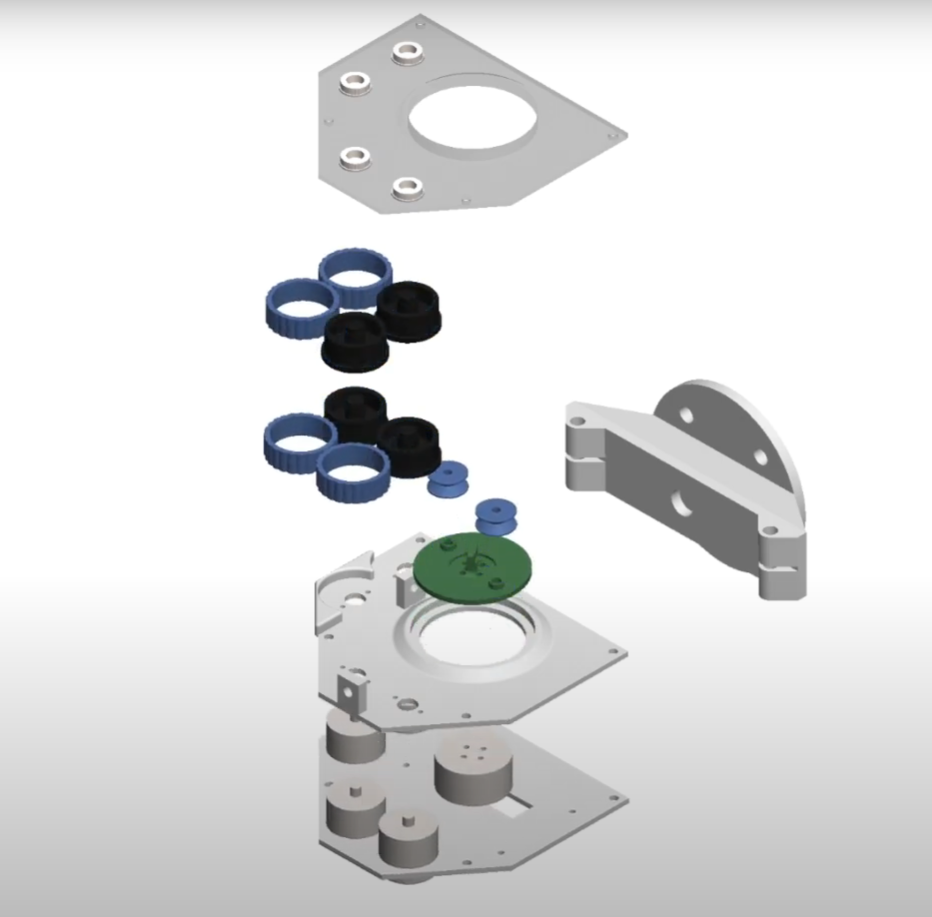
\includegraphics[width=1\columnwidth]{Figures/overall_img.png}
\caption{The SolidWorks designed hardware of the proposed gripper}
\end{minipage}
\end{tabular}
\end{figure}

Lasso Gripper comprises several crucial elements, including the robotic arm, controller, power supply, and communication interfaces. The robotic arm is engineered to provide the necessary degrees of freedom and precision required for accurate positioning and manipulation. The controller is responsible for managing the gripper's operations, processing sensor inputs, and executing the gripping actions. It employs advanced algorithms to ensure optimal performance. The power supply guarantees consistent electrical energy to all components, while communication interfaces enable seamless data exchange between the gripper and the central control system, ensuring synchronized operations.

\begin{figure}[htbp]
\centering
\begin{tabular}{cc}
\begin{minipage}[t]{0.9\textwidth}
\centering
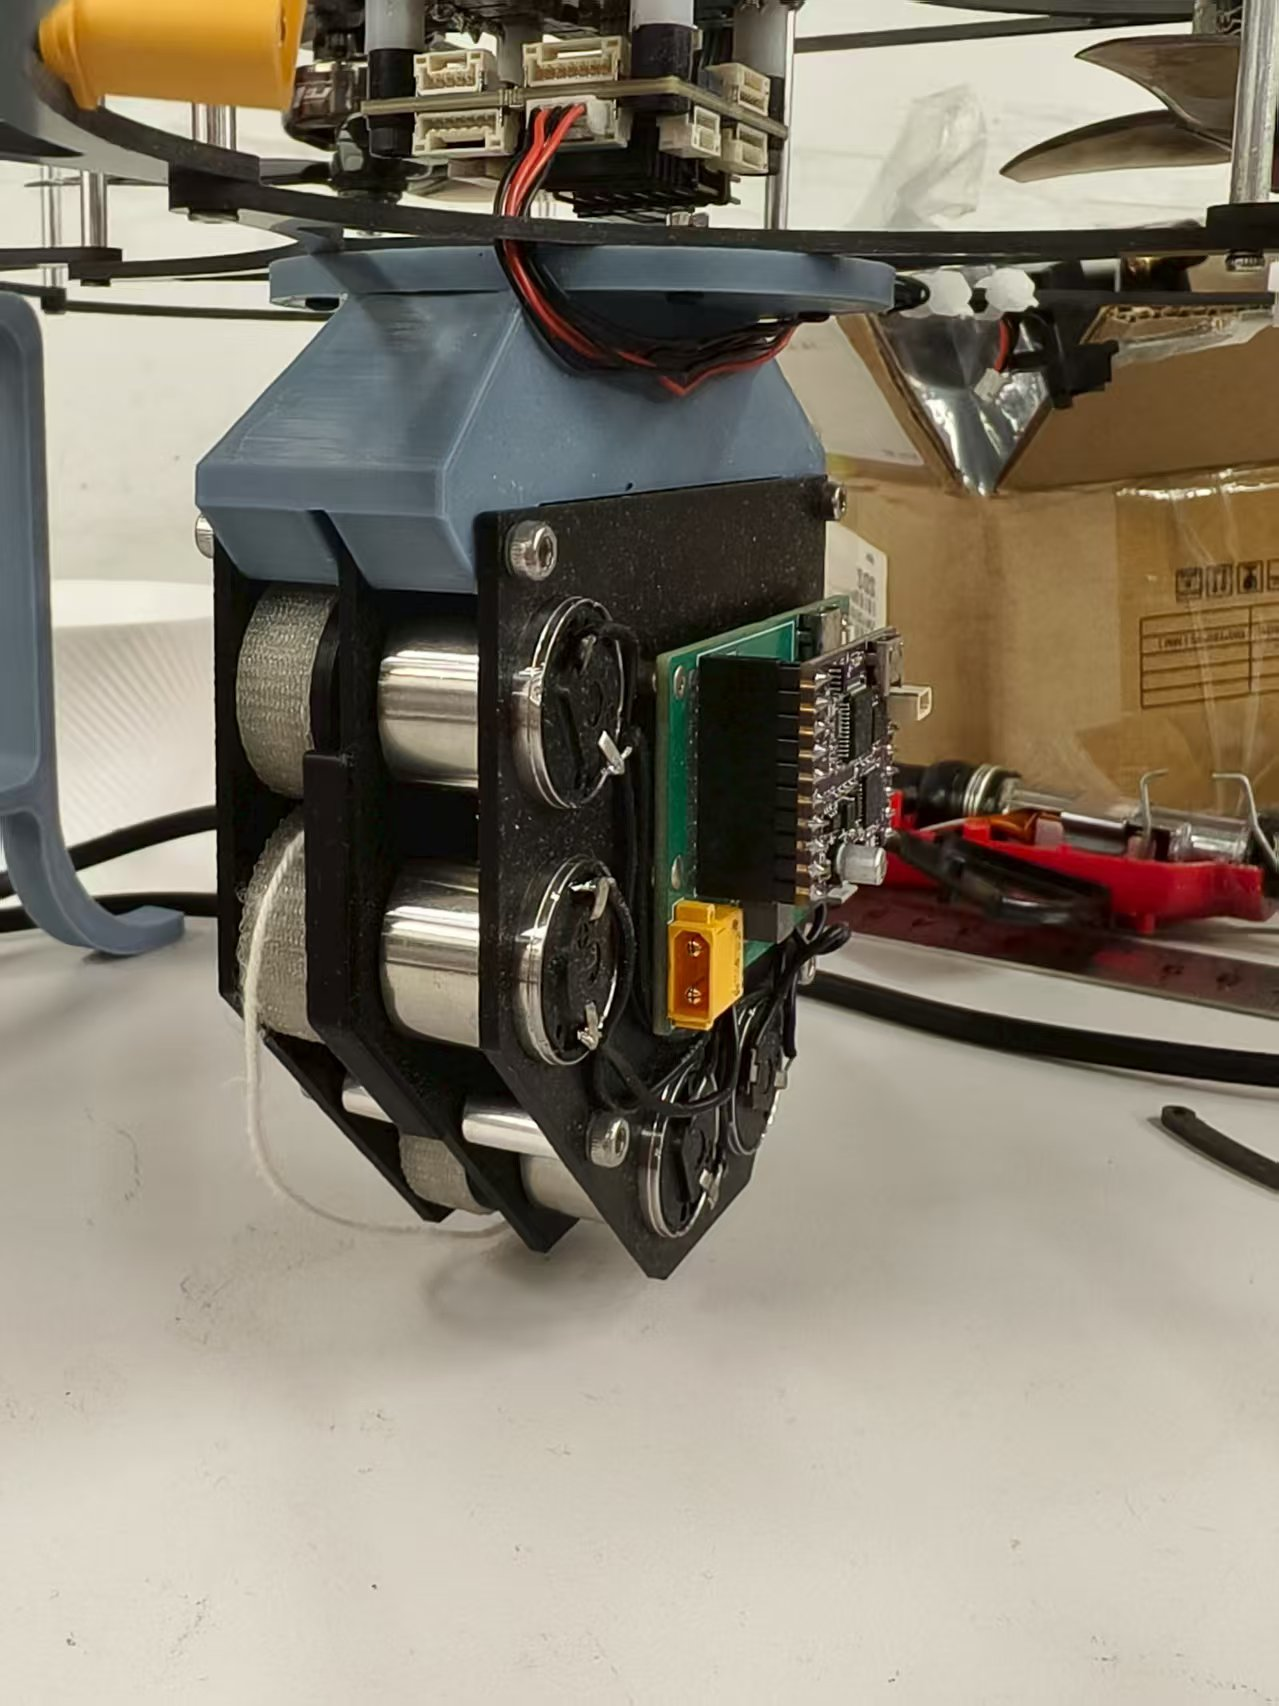
\includegraphics[width=1\columnwidth]{Figures/system_overview.jpg}
\caption{The proposed gripper connected with an ESP32 controller, motor electronic speed controller.}
\end{minipage}
\end{tabular}
\end{figure}



% ------------------------- 2.2 String Shooting and Retraction Mechanism -------------------------
\subsection{String Shooting and Retraction Mechanism}

The string shooting and retraction mechanism is a defining feature of Lasso Gripper, enabling it to perform complex gripping tasks with high efficiency. The mechanism comprises multiple components working in unison to achieve precise control over the string's movement.

The propulsion of the string is achieved through two pairs of friction wheels. These wheels are designed with high-friction surfaces to grip the string effectively. The wheels are driven by coreless motors with high speed so that the required rotational speeds for rapid string extrusion can be achieved\cite{murata2024elastic}.

During the string shooting phase, both pairs of friction wheels rotate in the same direction, propelling the string forward through a guided track. This track is meticulously designed to ensure the string forms a loop within the desired dimensions and shape. Sensors along the track monitor the string's position and velocity, providing real-time feedback to the controller.

\begin{figure}[htbp]
\centering
\begin{tabular}{cc}
\begin{minipage}[t]{0.9\textwidth}
\centering
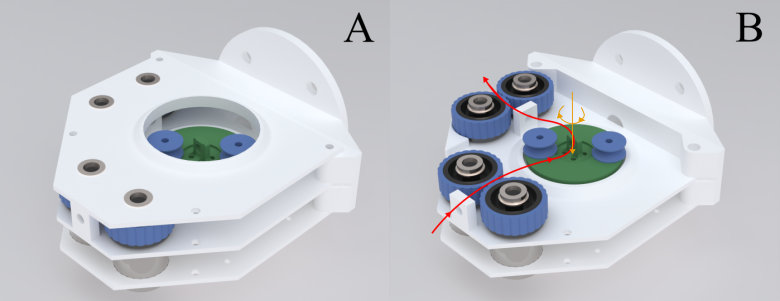
\includegraphics[width=1.0\columnwidth]{Figures/Figure11.png}
\caption{The friction wheels and the retraction mechanism driving motors are highlighted for illustration.}
\end{minipage}
\end{tabular}
\end{figure}

When retraction is required, the mechanism undergoes a coordinated sequence of actions. The rear pair of friction wheels maintains its rotational speed, continuing to pull the string inwards. Simultaneously, the front pair of wheels reverses direction, creating a counterforce that pulls the string loop into the space between the two pairs of wheels. This space is precisely designed to accommodate the retracted string without entanglement.

Within this confined space, a spool mechanism is designed. The spool is equipped with a rotational motor that winds the string onto itself, storing it neatly for future use. The tension exerted on the string during retraction is carefully controlled by a force feedback sensor located on the spool's axle. This sensor monitors the tension and adjusts the motor's torque to ensure that the object is gripped securely without applying excessive force that could cause damage.

\subsection{The ESP32 Main Controller for Lasso Gripper}

The ESP32 Main Controller serves as the central hub for managing the operations of Lasso Gripper. The ESP32 integrated Wi-Fi and Bluetooth capabilities, provides both the computational power and connectivity required for the gripper's complex functions.
\begin{figure}[htbp]
\centering
\begin{tabular}{cc}
\begin{minipage}[t]{0.5\textwidth}
\centering
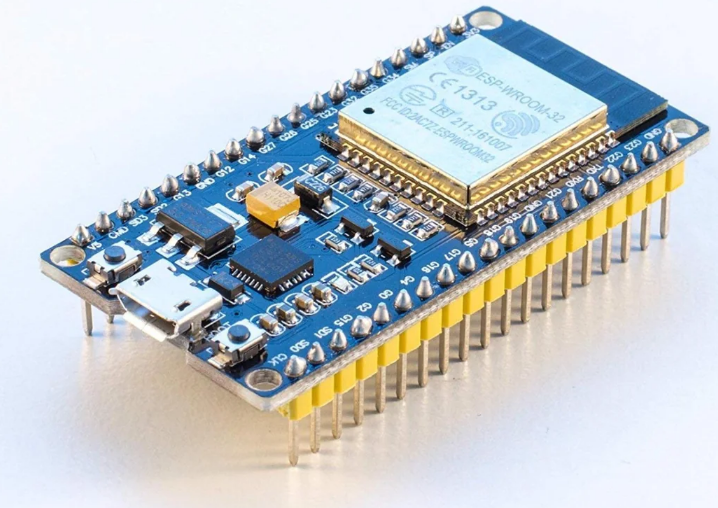
\includegraphics[width=1.0\columnwidth]{Figures/esp32.png}
\caption{The ESP32 controller used in the proposed Lasso Gripper.}
\end{minipage}
\end{tabular}
\end{figure}
At the heart of the ESP32 Main Controller is its dual-core processor, which efficiently handles multiple tasks simultaneously. This includes real-time processing of sensor data, executing gripping algorithms, and maintaining communication with external devices. The controller interfaces with various sensors, such as force sensors and motion trackers, to gather critical data on gripping forces, positioning accuracy, and object integrity.

The ESP32's GPIO (General Purpose Input/Output) pins are utilized to control the retraction modules that adjust the grasping force of the lasso, ensuring precise manipulation of objects. Additionally, the controller's PWM (Pulse Width Modulation) capabilities allow for fine-tuned control of the friction wheels.

The integrated Wi-Fi and Bluetooth features of the ESP32 facilitate seamless communication with a upper computer for target recognition and grasping planning. This connectivity also allows for remote monitoring and control, data logging, and integration with broader automation systems.

\section{Implications for Tendon-Driven Mechanisms and Medical Devices}

The Lasso Gripper work provides several mechanism-level insights that generalise beyond the specific prototype. First, the principle of using a flexible tensile element to create an adaptive capture region suggests new ways to trade capture range for control complexity. Second, differential and proximal actuation patterns enable low distal mass while still producing multi-degree-of-freedom effects at the end-effector; this trade-off is central to designing hand-held tools and remote manipulators. Third, performance metrics such as capture probability, peak tensile load, retraction dynamics, and hysteresis in the cable path form a compact evaluation set that is applicable to other tendon-driven designs.

These insights motivated the subsequent handheld surgical instrument presented in this thesis: the instrument intentionally reuses the same tendon-driven design philosophy and control principles, but applies them to the clinical constraints of minimally invasive surgery (low profile, ergonomic balance, safety and sterilizability). The following chapter therefore uses the Lasso Gripper both as a technical proof-of-concept and as a source of formalised mechanism design rules.

%% Chapter 4
\section{Gripping Algorithm Design} % Main chapter title
\label{Chapter4} % For referencing the chapter elsewhere, use 
The design of the gripping algorithm is critical to the functionality and efficiency of Lasso Gripper, ensuring precise and reliable manipulation of various objects. This section outlines the algorithm's design, which leverages advanced techniques for object recognition and manipulation, ensuring robust performance in diverse scenarios.

% ------------------------- 3.1 Object Recognition and Point Cloud Processing -------------------------
\subsection{}section{Object Recognition and Point Cloud Processing}
The gripping algorithm begins with the recognition of the target object using an Intel REALSENSE depth camera D435i. The camera captures a 3D point cloud of the object, providing detailed spatial information about its shape and orientation. The point cloud data is processed to identify key features of the object, including its boundaries, surface characteristics, and potential gripping points.

\begin{figure}[htbp]
\centering
\begin{tabular}{cc}
\begin{minipage}[t]{0.9\textwidth}
\centering
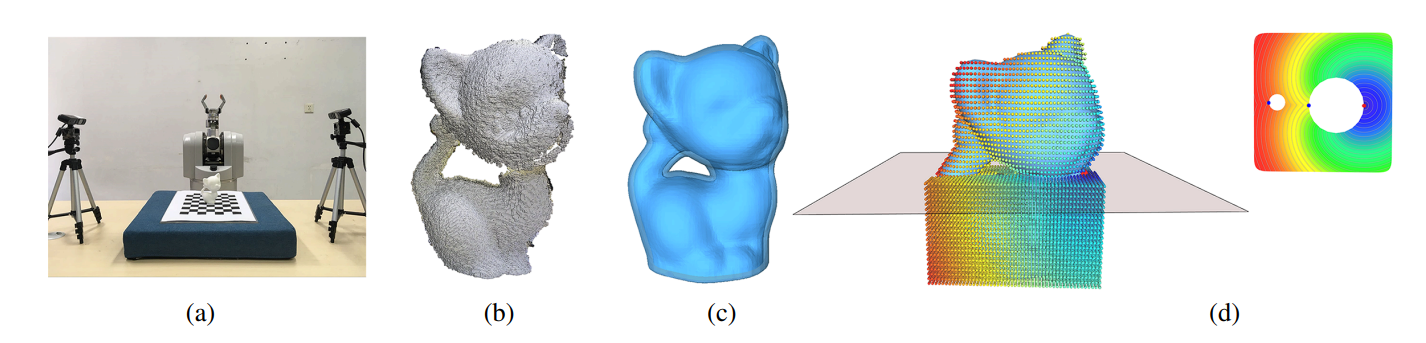
\includegraphics[width=1.0\columnwidth]{Figures/caging.png}
\caption{ The caging loop calculating algorithm for Lasso Gripper \cite{liu2018caging}. (a) The setup of the depth reconstruction system (b)The Point cloud captured by depth camera directly. (c) A r-offset surface is built for defining the grasping space. (d) Two Morse saddle points (blue) are calculated to define the grasping loop.}
\end{minipage}
\end{tabular}
\end{figure}

The algorithm employs a method for identifying the "neck" of the object, which is a critical region for secure gripping. The method entails identifying caging loops, which are closed curves characterized within the embedding space of the target object's shape \cite{liu2018caging}. By decoupling the caging loops from the surface geometry, the algorithm can synthesize feasible caging grasps that are not constrained by the object's surface details. This enables the gripper to handle objects with complex geometries and topologies effectively.

% ------------------------- 3.2 Loop Positioning and Tightening -------------------------
\subsection{Loop Positioning and Tightening}

Once the neck region is identified, the algorithm determines the optimal position for the string loop around the neck. The positioning is crucial for ensuring that the loop can be tightened securely without slipping or causing damage to the object. The algorithm calculates the precise coordinates for the loop's placement, taking into account the object's shape and the desired gripping force.

\begin{figure}[htbp]
\centering
\begin{tabular}{cc}
\begin{minipage}[t]{0.9\textwidth}
\centering
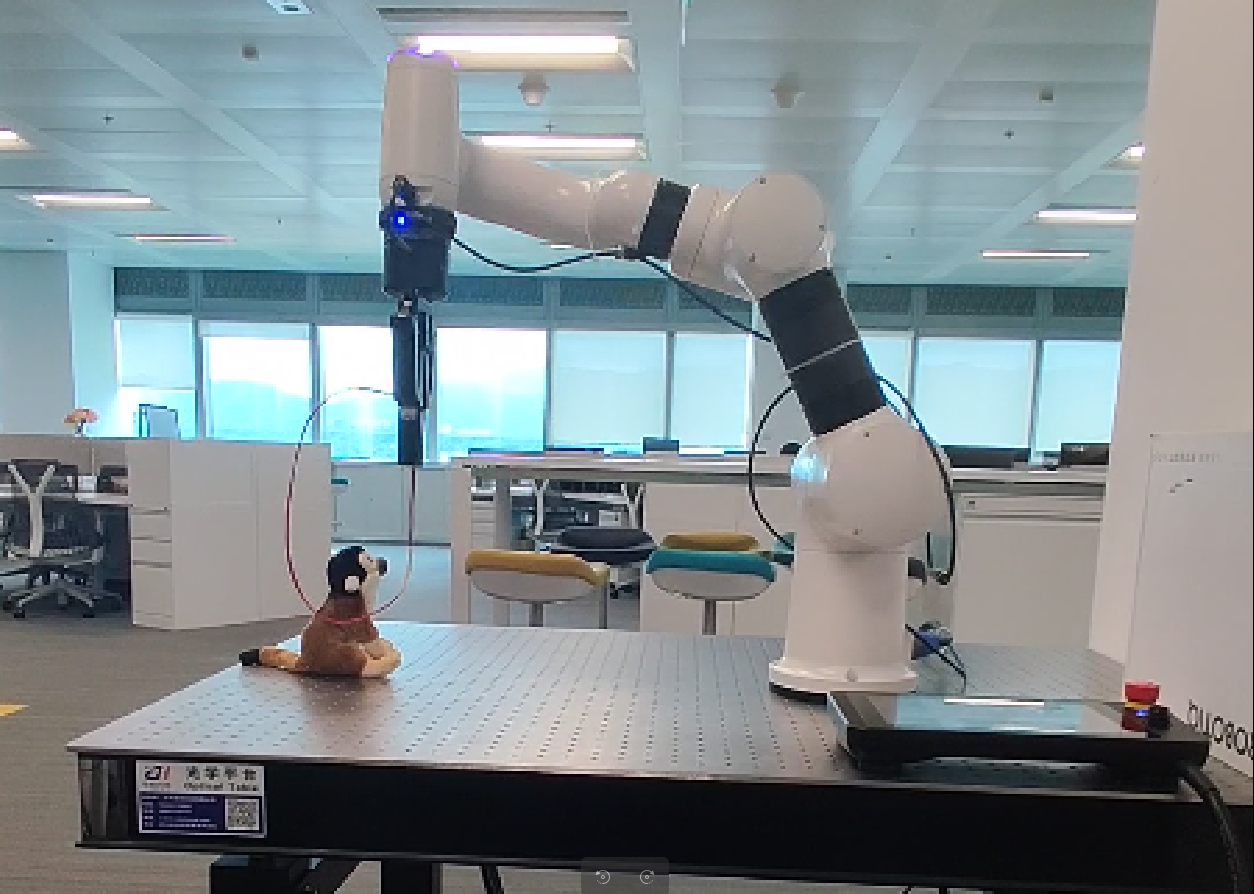
\includegraphics[width=1.0\columnwidth]{Figures/exp.png}
\caption{The illustration of the relative position of the string loop and the target object -- an early test}
\end{minipage}
\end{tabular}
\end{figure}

The tightening process is executed in a controlled manner, with the string loop gradually constricting around the neck region. The wrist of the gripper approaches the object in synchrony with the tightening action, ensuring that the loop maintains its position and grip. The following pseudo code illustrates the sequence of operations:

Input: Point Cloud P, String shooting velocity V

\begin{enumerate}
    \item Scan P using depth camera
    \item Process P to identify key features
    \item Identify neck region N in P using the caging loop method
    \item Determine optimal loop position L according to V 
    \item Align lower end of L with N
    \item Execute controlled tightening action
    \item Approach wrist towards object while maintaining loop position
\end{enumerate}

% ------------------------- 3.3 Real-Time Feedback and Adjustment -------------------------
\subsection{Real-Time Feedback and Adjustment}
The gripping algorithm incorporates real-time feedback mechanisms to adjust the gripping force and position dynamically. Sensors embedded in the gripper provide continuous data on the tension of the string, the position of the loop, and the force exerted on the object. This data is processed by the controller to make real-time adjustments, ensuring that the grip remains secure and stable.

The force feedback sensor, located on the spool's axle, plays a pivotal role in this process. It monitors the tension of the string during the tightening phase and adjusts the motor's torque accordingly. This prevents excessive force that could damage the object and ensures that the grip is firm enough to hold the object securely.
\let\cleardoublepage\clearpage
%% Chapter 5
\section{Dynamics of the String Loop} % Main chapter title

%\label{Chapter5} % For referencing the chapter elsewhere, use 

\subsection{The Dynamics of String Analysis}
The dynamics of the string loop in the lasso gripper are rooted in principles of fluid mechanics and physics \cite{abello2024string}\cite{daerr2019charmed}. This section explores the behavior of the string loop as it transitions from a low-velocity, gravity-dominated state to a high-velocity, self-supporting configuration.

At low velocities, the string loop is primarily influenced by gravity, causing it to hang downwards. This gravity-dominated regime is characterized by a noticeable sag in the string due to its light. As the velocity increases, the string undergoes a transition to a high-velocity regime where it forms a self-supporting loop. In this regime, the string is no longer suspended due to inertia but rather through the hydrodynamic drag. This drag force exerted by the surrounding air counteracts gravity, allowing the string to maintain a stable loop shape.

\begin{figure}[htbp]
\label{simulation}
\centering
\begin{tabular}{cc}
\begin{minipage}[t]{0.9\textwidth}
\centering
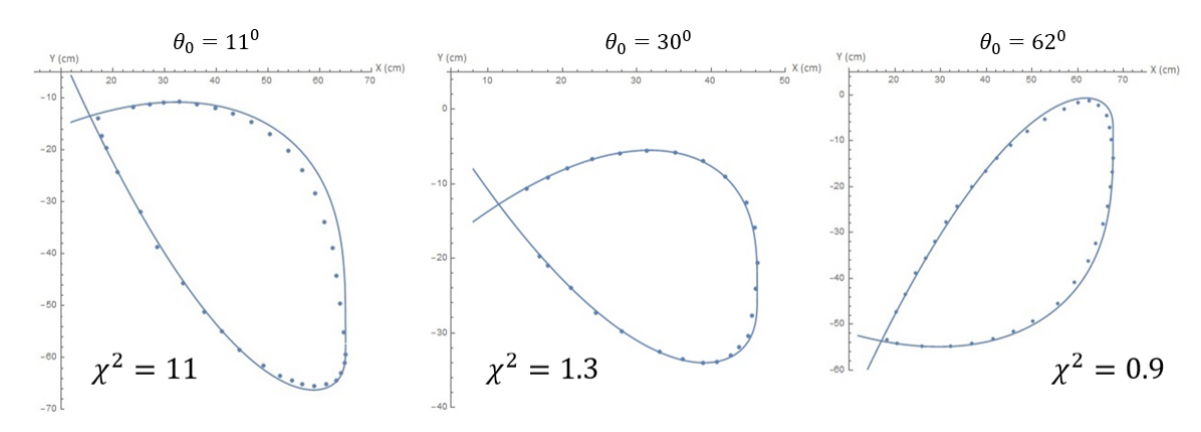
\includegraphics[width=1.0\columnwidth]{Figures/stringsim.png}
\caption{The string loop curve fitting of numerical theoretical solution with experimental profiles \cite{abello2024string}. In this case, the linear mass $\mu = 0.283 \pm 0.005 g \cdot \: m^{-1}$,  the length of the string loop $L = 160 \: cm$, shooting velocity $v = 5.1 \: m \cdot s^{-1}$ and sevel values of ejection pitch angle $\theta _0$. A satisfactory fitting result with $\chi^2 \leq 11$ is obtained.  }
\end{minipage}
\end{tabular}
\end{figure}

Assuming the loop junction is at position $s = s_0$ when $t = 0$, the position of the junction along this curve is $s = v \cdot t + s_0 (\mathrm{mod} \, L) $. $T(s)$ is noted as the tension. Frenet-Serret frame $(\vec {\tau}, \vec {n})$ is used to describe the dynamics of an infinitesimal piece of string of length $\mathrm{d}s$ subjected to its ight $\mu \mathrm{d} s \vec {g}$, its tension $\frac{\mathrm{d}(T \vec {\tau})}{\mathrm{d}s}\mathrm{d}s^3$ and the linear air drag $-f \vec {\tau} \mathrm{d} s$ where $f>0$.

Newton's motion equation produces:

\vspace{-0.3cm}
\begin{equation}
\begin{split}
\frac{\mathrm{d}(\mu v \vec {\tau})}{\mathrm{d}t} = \mu \vec {g} + \frac{\mathrm{d}(T \vec {\tau})}{\mathrm{d}s} - f \vec {\tau}
\end{split}
\end{equation}

Noting that $\mathrm{d}s = v \cdot \mathrm{d}t$, defining the effective tension $T^o = T-\mu v^2$, and recalling that $\vec {\tau} = \frac{\mathrm{d}\vec {\tau}}{\mathrm{d}s}$, the following can be obtained:

\vspace{-0.3cm}
\begin{equation}
\begin{split}
T^o \vec {\tau} - f \vec {\tau} +\mu \vec {g}s=\vec {0}
\end{split}
\end{equation}

If the origin is wisely chosen for $\vec {r}$ as the point $o$  where the tangent to the loop is vertical, the integration constants will vanish. In the vertical local FrenetSerret frame, defining $tan \theta = \frac{\mathrm{d}z}{\mathrm{d}x}$, the following can obtained:

\vspace{-0.3cm}
\begin{equation}
\begin{split}
-f \cdot ( x \mathrm{tan} \theta - z )+\mu gs=0
\end{split}
\end{equation}

This integro-differential equation can be solved analytically as figure 4.1.

The formation of the self-supporting loop is governed by the hydrodynamic drag acting on the string. Daerr et al. (2019) investigated this drag both experimentally and theoretically, focusing on a smooth long cylinder moving along its axis \cite{daerr2019charmed}. The drag force is a result of the interaction beten the moving string and the air, creating a pressure differential that lifts and supports the string loop.

The equations that characterize the shape of the string loop re formulated under the assumption of an infinitely small string radius. These equations unveil a pivotal juncture, delineating two distinct regions: a supercritical region where the wave speed along the string is less than the string's own speed, and a subcritical region where the wave speed surpasses the string's speed. This critical juncture at the interface of these regions is vital to the string loop's dynamics. Solutions to the loop equations that remain regular at this critical juncture have been derived and subsequently compared to experimental data.

In practical terms, understanding the string loop dynamics has significant implications for the lasso gripper's design and operation. By leveraging the principles of hydrodynamic drag and the transition beten different velocity regimes, the lasso gripper can achieve precise control over the string loop's shape and stability. This enables the gripper to handle objects with varying sizes and shapes effectively, ensuring a secure and reliable grip.

\section{The workspace analysis}
Due to the self-supporting loop configuration of the Lasso Gripper in three-dimensional space, the operational workspace of the proposed manipulator significantly exceeds the physical reach of the robotic arm.

\begin{figure}[ht]
    \centering
    
\includegraphics[width=0.8\linewidth]{workspace.png} 
    \caption{Lasso Gripper string loop is set at the end of UR5 robotic arm. The green point at the end of the robotic arm marks the position reachable by a rigid manipulator, while the red point indicates the furthest position on the string loop from the original point at the same robotic position.}
    \label{ws1}
\end{figure}

As delineated in Section 5.1, the three-dimensional pose kinematics of the lasso-type end-effector can be characterized by constrained dynamics under gravitational loading. For the local coordinate system constrained by gravity, the working plane is defined as the plane formed by the lasso's ejection direction and the gravity direction. The rotation with the normal vector of this working plane as the rotation axis is defined as pitch, while the rotation with the gravity vector as the rotation axis is defined as yaw. According to the right-hand coordinate system, the roll rotation axis is defined as the axis orthogonal to both the pitch and yaw rotation axes, lying within the working plane. Specifically, the gripper mechanism exhibits negligible roll angular displacement within the global coordinate frame due to gravitational stabilization. Its pitch orientation becomes parametrically dependent on the projectile's ejection velocity vector, while yaw angle variations are governed by the robotic manipulator's pose in Cartesian space.

\begin{figure}[htp]
    \centering
    
\includegraphics[width=0.6 \linewidth]{ws3.jpg} 
    \caption{The initial robotic arm workspace is marked in green and extended Lasso Gripper workspace is marked in red.}
    \label{ws2}
\end{figure}

A case study is conducted with specific parameters to investigate the working space of the Lasso Gripper on a 6-axis robotic arm using the Monte Carlo method. A UR5 robot without joint angle limitation is applied as an example in Fig. \ref{ws1}, and $[R, x_{+}, x_{-}]$ is set as $[0.7, 0.2m, 0.1m]$ in this case. The green point at the end of the robotic arm is the specific position that a rigid manipulator can reach, and the red point represents for the furthest point to the original point on the string loop at the same robotic position. The set of green points and red points in Fig. \ref{ws2} is the workspace of the robotic arm and the extended lasso gripper, respectively. Generating 200,000 sampling points for robotic arm configuration, the volume of workspace convex hull is calculated. The volume of the original UR5 workspace convex hull is $3.4620 m^3$ , and the volume of the extended Lasso Gripper workspace convex hull is $8.9002 m^3$. The workspace extending ratio is up to $157.08\%$.

%% Chapter 6
\section{Experimental Validation (Qualitative Demonstrations)} % Main chapter title

%\label{Chapter6} % For referencing the chapter elsewhere, use


\subsection{Objectives}
To validate the unique capabilities of Lasso Gripper and compare its performance with antipodal grippers, the following experimental procedure was designed. The setup employed a modular robotic arm (Inovo Robotic) with a maximum payload of 6 kg, mounted on a flat platform where the target objects were placed.
The experimental objectives were divided into four categories:

    \begin{enumerate}
        \item Capturing animal figures by the neck or horns,

        \item Capturing objects of diverse shapes,

        \item Capturing oversized objects through shape adaptation, and

        \item Capturing moving objects.
    \end{enumerate}

\subsection{Experimental Setup}
For Objectives 1 to 3, the procedure consisted of the following steps:

    \begin{enumerate}
        \item The robotic arm moved to a predefined position to initiate the launch phase;

        \item Lasso Gripper was swept toward the target while maintaining its open-loop configuration;

        \item Upon reaching the target, the string was retracted to secure the object;

        \item The arm performed a vertical lifting motion while maintaining a stable grip.
    \end{enumerate}
For Objective 4, the robotic arm remained stationary, and Lasso Gripper independently executed the capture process aimed at intercepting a moving object in flight.
\subsection{Experimental Procedure}
The experimental procedure will be divided into several phases to thoroughly evaluate Lasso Gripper's performance:
\begin{enumerate}
    \item \textbf{Static Object Gripping Tests}:
            In the second phase, static object gripping tests will be conducted to assess the gripper's ability to handle static objects. Test objects will be placed in fixed positions, and the gripping algorithm will be executed to secure and lift each object. Success rates, gripping forces, and any slippage or deformation of the objects will be meticulously recorded.

\item \textbf{Dynamic Object Gripping Tests}:
The third phase will focus on dynamic object gripping tests to evaluate the gripper's performance with moving objects. Test objects with controlled motion, such as rolling or sliding, will be introduced, and the lasso will attempt to grip them. The effectiveness and speed of the gripping action will be measured to determine the gripper's capability in dynamic scenarios.

\item \textbf{Comparative Analysis}:
Finally, a comparative analysis will be conducted to compare Lasso Gripper's performance with traditional gripping methods. Parallel tests using a standard parallel-jaw gripper will be carried out on the same set of test objects. Differences in gripping force, handling precision, success rates, and overall efficiency will be analyzed to highlight the advantages and potential areas for improvement of Lasso Gripper.
\end{enumerate}


\section{Data Collection and Analysis}
Data collection involved capturing both quantitative and qualitative metrics where available. Key measurements included gripping force (recorded via force sensors) and positioning accuracy (assessed with motion tracking to evaluate loop placement around candidate neck regions). Where feasible, counts of successful and failed grasps were noted; however, the evaluation emphasis in this chapter is demonstrative rather than a full statistical study. Object integrity was inspected for visible damage or deformation after handling, and common failure modes were logged to guide subsequent design iterations.

Limited summary statistics were computed where appropriate, but a comprehensive statistical campaign (large-sample success rates, fatigue tests) is outside the present scope and is recommended for future work.

\section{Results And Discussion}
\noindent
The evaluation reported in this chapter is demonstration-focused and intended to validate feasibility, illustrate common operating modes, and highlight comparative behavior versus conventional antipodal grasping. Test cases emphasized scenarios where a loop-based capture offers clear mechanical advantages. Results are presented as illustrative sequences and representative frames rather than as full statistical studies. Observed failure modes (entanglement, missed captures at extreme approach angles, and tension-management lapses) are documented to guide design improvements.
\subsection{Various Objects Grasping Results}
\begin{figure}[htbp]
    \centering
    
\includegraphics[width=0.7 \linewidth]{test3.png}
    \caption{Validation of grasping ability via bull and horse figures.}
    \label{fig:3}
\end{figure}

\begin{figure}[htbp]
    \centering
    
\includegraphics[width= 0.7 \linewidth]{test1.png}
    \caption{Validation of grasping ability over variable shapes: drone, cabbage, coke can and chili pepper.}
    \label{fig:4}
\end{figure}

\begin{figure}[htbp]
    \centering
    
\includegraphics[width=0.7 \linewidth]{test2.png}
    \caption{Validation of grasping ability with oversized objects: inflated balloons.}
    \label{fig:5}
\end{figure}
Fig. \ref{fig:3} illustrates the experiments result for Aim 1. The lasso was successfully attached to the horn and the neck, respectively, and firmly grasped them towards the tip of the robotic arm, transporting the figures from the platform. For the second set of target objects, a drone, a cabbage, an empty coke can and a chili pepper were selected. In Fig. \ref{fig:4}, Lasso Gripper successfully grasped the targets and carried it away from the base.
\begin{figure}[htbp]
    \centering
    
\includegraphics[width=0.7 \linewidth]{test4.png}
    \caption{Flying object is captured by Lasso Gripper.}
    \label{fig:6}
\end{figure}
The grasping strategy for these two experiments is similar. For both cases, the robotic swept right above the target while Lasso Gripper maintained the string in full range, ensuring that the target could be captured as the string retracted. This grasping strategy can also be extended to other expansive grasping targets, such as oversized balloons. Hence, the third set of objects are two flower-shaped balloons, with diameters of 45cm and 71cm, respectively, and a spike ball with a diameter of 18cm, as shown in Fig. \ref{fig:5}. Though Lasso Gripper could not fully grasp the balloons due to the limitation in the string, it still firmly secured the balloons and lifted off the platform. This laid the foundation for the fourth case of the experiment, which was to capture flying objects. Fig. \ref{fig:6} presented the experiment by manually throwing one long balloon and the small flower balloon through the string made by Lasso Gripper.

Some interesting phenomena were observed during the demonstration, revealing more advantages of Lasso Gripper. Firstly, the string's sustained high speed makes it possible to grasp objects close to the table. In Fig. \ref{fig:4} (B) and Fig. \ref{fig:4} (D), where the cabbage and chili pepper are put very close to the table, Lasso Gripper can still maintain the loop shape and achieve the grasping task. The same goes for the demonstration near a wall. Secondly, the adaptive force closure of the string allows a certain degree of deviated grasping position to be tolerated. Compared with the grasping attitude in Fig. \ref{fig:5} (D), the string loop pose in Fig. \ref{fig:5} (C) occurs an unexpected deviation. Lasso Gripper realizes an adaptive force-closure grasping.

\subsection{Comparisons with Antipodal Point Gripper}

\begin{figure}[htbp]
    \centering
    
\includegraphics[width=0.7 \linewidth]{compare.png}
    \caption{The inflated balloon is captured by the antipodal gripper. As a result of the concentrated stress applied, the balloon was severely deformed.}
    \label{fig:7}
\end{figure}
As the comparison group, the 2F-140 gripper from Robotiq was used as the classical antipodal gripper. In this scenario, the small flower balloon was used as the target due to its elasticity under external forces. As demonstrated in Fig. \ref{fig:7}, the flower balloon was clearly under dramatic deformation as the antipodal gripper tried to pick it up from the platform. Though the balloon remained intact after the experiment instead of an explosion, the limitations of traditional grippers on handling delicate or plastic objects are straightforward. Instead of directly applying forces and pressure over the surface of the target, Lasso Gripper captured objects via rope tension, avoiding causing damage to the objects. Moreover, this unique feature enables Lasso Gripper to capture larger and potentially heavier objects than traditional grippers.

Taken together, these experiments validate Lasso Gripper not only as a novel end-effector, but also as a mechanism study platform for tendon-driven manipulation. The results show that controlled tension, distributed contact, and low-distal-complexity actuation can produce robust behavior under uncertainty in object size, shape, and motion. The next part of this thesis transfers these mechanism insights to a more constrained setting, where the same tendon-driven principles must satisfy the stricter requirements of hand-held surgical instrumentation.

%% Chapter 7
\chapter{Innovative Design of a Handheld Surgical Instrument Balancing Weight and Functionality} % Main chapter title

\label{Chapter7} % For referencing the chapter elsewhere, use 

\section{Necessity To Develop Handheld Motorized Medical Instrument}
As established in prior discussions, contemporary research in surgical robotics has predominantly prioritized maximizing tip-positioning accuracy through advanced actuation methods and the integration of supplementary sensors. While these approaches demonstrably enhance precision, they often overlook a critical practical constraint: the weight-to-functionality ratio. The evident correlation between enhanced capabilities—achieved through more powerful motors or additional sensing—and increased instrument mass creates a significant adoption barrier. This added weight often leads surgeons to favor simpler, nearly weightless traditional instruments over their motorized counterparts, despite the latter's technological advantages.

To resolve this fundamental trade-off, the present work introduces a holistic approach to ergonomic and functional design in robotic-assisted surgery. This chapter details the conception, design, and implementation of a novel structured handheld instrument that strategically balances mass, functionality, and clinical usability. The proposed system embodies a dedicated effort to distribute system components intelligently, minimize inertial load, and integrate multi-modal sensing without compromising the manipulator's agility or the surgeon's comfort. By fundamentally re-evaluating the instrument architecture from a human-centric perspective, this research aims to deliver a platform that surgeons are not only able to use, but genuinely prefer to use, thereby bridging the gap between technological potential and clinical practicality.
%During the research and development of the Lasso Gripper, the functional principles of cables or ropes were extensively investigated, particularly in terms of their purpose and form when configured as a loop. Conventionally, a loop is formed by tying or securing a string, allowing object capture primarily through adjustments in the loop size. This method relies heavily on the motor's ability to execute rapid and precise grasping motions. Furthermore, the repeatability and consistency of such a system are strongly dependent on the design and performance of the launch and retraction mechanism.

%However, an innovative approach involves dividing the loop into two separate strands. By cutting the loop, two independent strings are created, each capable of applying tensile forces—pulling rather than pushing—on a target object. When these two strings are attached to opposite sides of an object and actuated in differentiated directions, they can generate in-plane rotational movements. This significantly enhances the dexterity and functionality of the system, enabling more complex manipulations such as rolling, reorienting, or stabilizing objects without requiring additional mechanical components.

%This concept is particularly relevant in the context of cable-driven hand-held medical devices. Such devices often require high precision, flexibility, and minimal invasive manipulation, especially in surgical or diagnostic applications. For instance, in laparoscopic tools, the use of dual-string actuation can allow for finer tip articulation and rotational control, improving the surgeon’s ability to navigate and interact with tissue in confined spaces. The tension-based control also offers inherent compliance and force feedback, which are critical for safe interaction with delicate biological structures. By utilizing the properties of the string, such medical instruments can both maintain a high force-volume ratio at the tip of the instrument while keeping a low profile in its size.

\section{Core Design Advantages for Hand-Held Applications}

This cable-driven, differential actuation philosophy offers several fundamental advantages that are particularly suited to the development of advanced hand-held devices:
    
    -\textbf{Enhanced Dexterity and Manipulation}: The system enables multi-degree-of-freedom manipulation (e.g., rotation, twisting) using a minimal number of actuated elements. This is crucial for applications requiring fine motor control within confined spaces.

    -\textbf{Inherent Compliance and Safety}: The system is naturally compliant. Cables under tension provide a direct force-feedback path. If an unexpected obstacle is encountered, the cables will slacken rather than apply a rigid, potentially damaging force. This passive safety feature is a critical asset for interactions in unstructured or delicate environments.

    -\textbf{Proximal Actuation and Minimal End-Effector Mass}: A primary benefit for hand-held device design is the ability to locate the heavy actuators (motors) and associated drive electronics proximally, either in the device's handle or even in a remote unit. This dramatically reduces the mass and inertia of the distal end-effector, leading to improved ergonomics, reduced user fatigue, and the potential for higher maneuverability and smaller form factors at the interaction point.

\section{Defining Performance Metrics for Structural Design}

To translate this conceptual framework into a viable product, key performance metrics must be established. These metrics will directly guide the structural design choices detailed in the subsequent chapter:

    -\textbf{Precision and Resolution}: The minimum achievable incremental movement of the end-effector tip, targeting sub-millimeter and sub-degree accuracy for delicate tasks.

    -\textbf{Force Capability}: The maximum tensile force the cables must transmit to securely grasp and manipulate objects of a target weight range.

    -\textbf{Range of Motion}: The required angular deflection and rotational range of the end-effector to perform its intended functions effectively.

    -\textbf{Force Transmission Efficiency}: Minimizing friction losses throughout the cable drive path is essential for accurate force feedback and predictable control.

    -\textbf{Low Hysteresis and Backlash}: The structural design must ensure minimal play and elastic deformation in the system to guarantee precise, repeatable, and immediate response to actuator inputs.

\section{Pathway to Structural Implementation}
This chapter has outlined the conceptual leap from a simple loop to a differentially actuated cable-driven system, highlighting its inherent advantages for dexterous manipulation in hand-held applications. The core principles of compliance, proximal actuation, and differential control form the foundation upon which a physical device must be built.

The following chapter will address the critical task of transforming this concept into a robust mechanical reality. The structural design must meticulously integrate several key subsystems:
\begin{enumerate}
    \item \textbf{Actuation Unit Selection and Layout}: Choosing motors and sensors that meet the performance metrics and determining their optimal arrangement.

    \item \textbf{Cable Routing and Guidance System}: Designing low-friction, precise pathways for the cables to ensure efficient force transmission and longevity.

    \item \textbf{End-Effector Configuration and Cable Termination}: Engineering the interface where the cables attach to the manipulator, ensuring secure anchoring, precise motion, and mechanical advantage.

    %\item \textbf{Ergonomic Handle and Housing Design}: Packaging the system into a form factor that is balanced, comfortable, and intuitive for the user to hold and operate over prolonged periods.
\end{enumerate}
Through this structured approach, the subsequent design will validate the conceptual advantages discussed herein and realize a functional, high-performance cable-driven hand-held device.

\subsection{Relation to the Lasso Gripper and Mechanism-Focused Thesis}

The design choices described in this chapter were strongly influenced by the earlier development of the Lasso Gripper. Rather than treating the handheld instrument as an isolated engineering project, this work positions the instrument as a second application that tests and extends mechanism-level hypotheses derived from the Lasso Gripper: that tensile elements can be used to increase capture adaptivity, that differential tendon routing produces compact multi-DOF behaviour, and that proximal actuation enables low distal inertia. Emphasising these commonalities keeps the thesis focused on theoretical and design principles for tendon-driven mechanisms, while using concrete device implementations to validate those principles.
%\include{Chapters/07_instrument_mechanics}
%% Instrument control and HMI (formerly chapter9.tex)

% Chapter Template

%\section{Control Strategy} % Main chapter title

%\label{Chapter9} % For referencing this chapter elsewhere, use

%----------------------------------------------------------------------------------------
%\tSECTION 1
%----------------------------------------------------------------------------------------

\section{Control Strategy and Implementation}
\subsection{Modeling}

The project aims to implement a da Vinci–style surgical instrument claw effect using a compact 4-DoFs hardware architecture: a 3-DoFs manipulator arm plus a single gripper open/close degree of freedom. The system input is provided by the handle as three rotational joint angles and one gripper opening angle.

Since the manipulator itself has only three actual mechanical degrees of freedom, it cannot realize an arbitrary rotation axis in space. A specified direction in space requires three independent pose parameters, and a stable pose also consumes three degrees of freedom. This makes the system inherently over-constrained if arbitrary axis rotation is demanded. In contrast, the da Vinci system achieves effective 6-DOF stabilized control by using a larger arm to drive a smaller wristed arm in coordinated motion. Under the hardware constraints of this project, that six-degree-of-freedom stabilization strategy is not considered.

Instead, the control design adopts a decoupled attitude mapping. The coordinate system is defined using Euler angles to describe the desired end-effector orientation. The input attitude from the handle is mapped linearly to the output attitude of the manipulator, subject to the arm's three-degree-of-freedom limitations.


\subsection{Denavit–Hartenberg Coordinate Frames}
The coordinate frames are established using standard Denavit–Hartenberg conventions, as shown in Figures~\ref{fig:dhcord} and~\ref{fig:dhcord1}. The manipulator consists of three rotary joints, with the following D-H parameters:

\begin{table}[htbp]
    \centering
    \caption{Denavit–Hartenberg parameters for the 3-DoF manipulator}
    \label{tab:dhparams}
    \begin{tabular}{c c c c c l}
        \toprule
        Link & $\theta_i$ & $d_i$ & $a_i$ & $\alpha_i$ & Remarks \\
        \midrule
        1 & \(\theta_1\) & 0 & 0 & \(-90^\circ\) & Base rotation \\
        2 & \(90^\circ - \theta_2\) & 0 & \(-a_2\) & \(90^\circ\) & Upper arm rotation \\
        3 & \(\theta_3 - 180^\circ\) & 0 & \(a_3\) & 0 &  \\
        \bottomrule
    \end{tabular}
\end{table}

And the following Rotation Matrix for the end-effector orientation:
\[
A_1 =
\begin{bmatrix}
c_1 & 0 & -s_1 & 0 \\
s_1 & 0 & c_1 & 0 \\
0 & -1 & 0 & 0 \\
0 & 0 & 0 & 1
\end{bmatrix},
\qquad
A_2 =
\begin{bmatrix}
s_2 & 0 & c_2 & -a_2 s_2 \\
c_2 & 0 & -s_2 & -a_2 c_2 \\
0 & 1 & 0 & 0 \\
0 & 0 & 0 & 1
\end{bmatrix},
\qquad
A_3 =
\begin{bmatrix}
-c_3 & -s_3 & 0 & -a_3 c_3 \\
s_3 & -c_3 & 0 & a_3 s_3 \\ 
0 & 0 & 1 & 0 \\
0 & 0 & 0 & 1
\end{bmatrix}
\]
The end-effector pose is governed by the following equations:
\begin{align*}
P_x &= c_1 s_2(-a_3 c_3) + (-s_1)(a_3 s_3) + c_1 c_2(0) + (-a_2 c_1 s_2) \\
& \rightarrow P_x= -a_3 c_1 s_2 c_3 - a_3 s_1 s_3 - a_2 c_1 s_2 \\
P_y &= s_1 s_2(-a_3 c_3) + c_1(a_3 s_3) + s_1 c_2(0) + (-a_2 s_1 s_2) \\
& \rightarrow P_y= -a_3 s_1 s_2 c_3 + a_3 c_1 s_3 - a_2 s_1 s_2 \\
P_z &= -c_2(-a_3 c_3) + 0(a_3 s_3) + s_2(0) + a_2 c_2 \\
& \rightarrow P_z= a_3 c_2 c_3 + a_2 c_2
\end{align*}
The orientation of the end effector can also be expressed through the base axis direction vectors shown in Table~\ref{tab:axisdir}.

\begin{table}[htbp]
\centering
\caption{End-effector base-axis direction vectors}
\label{tab:axisdir}
\begin{tabular}{|l|l|l|l|}
\hline
\textbf{Direction} & \textbf{X-axis  ($n$)} & \textbf{Y-axis  ($o$)} & \textbf{Z-axis  ($a$)} \\
\hline
Base X-axis & $-c_1 s_2 c_3 - s_1 s_3$ & $-c_1 s_2 s_3 + s_1 c_3$ & $c_1 c_2$ \\
\hline
Base Y-axis & $-s_1 s_2 c_3 + c_1 s_3$ & $-s_1 s_2 s_3 - c_1 c_3$ & $s_1 c_2$ \\
\hline
Base Z-axis & $c_2 c_3$ & $c_2 s_3$ & $s_2$ \\
\hline
\end{tabular}
\end{table}

\begin{figure}[htbp]
    \centering
    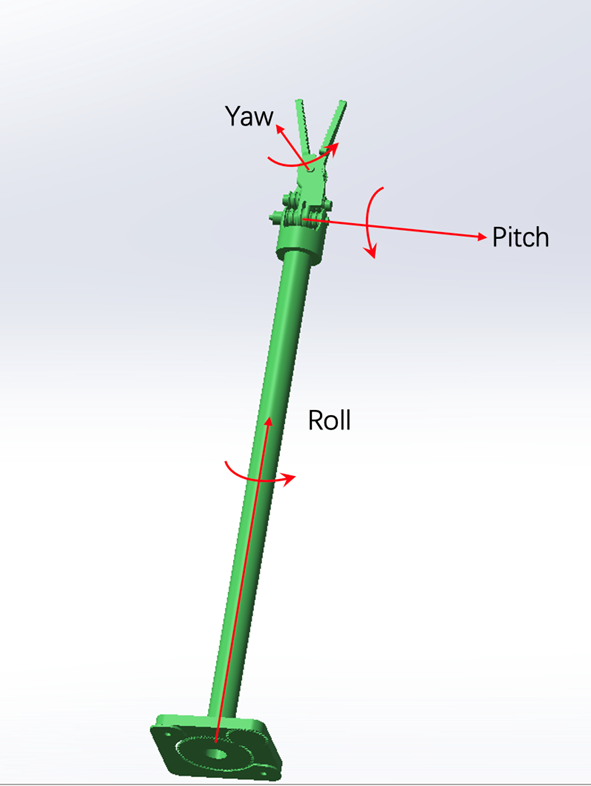
\includegraphics[width=0.8\linewidth]{Figures/DH cord1.png}
    \caption{Denavit–Hartenberg coordinate frame definition for the manipulator}
    \label{fig:dhcord}
\end{figure}

\begin{figure}[htbp]
    \centering
    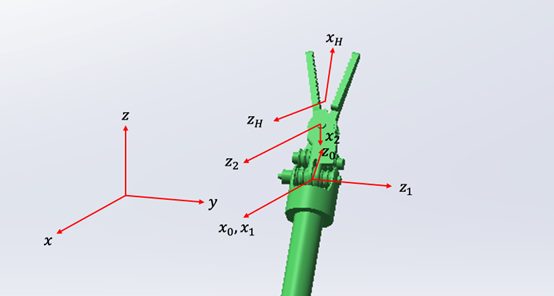
\includegraphics[width=0.8\linewidth]{Figures/DH cord.png}
    \caption{Alternative view of the D-H coordinate frames and joint axes}
    \label{fig:dhcord1}
\end{figure}

\subsection{System Architecture and Data Flow}
The control system is implemented on an ESP32 microcontroller running FreeRTOS, enabling real-time processing of sensor inputs and actuator commands. The architecture follows a cyclic loop structure, as illustrated in the firmware code, where sensor feedback is continuously acquired, processed, and translated into motor commands.

At the core of the system is a feedback loop that reads position, speed, load, voltage, temperature, and current from eight Feetech STS-series servos via UART communication. This multi-modal feedback provides the foundation for state estimation and control. The input module captures user intent through four degrees of freedom: wrist yaw, pitch, roll, and gripper opening/closing, using AS5600 magnetic encoders and STS3009 servos for precise motion detection.

\subsection{Intent Estimation and Command Mapping}
User inputs are mapped from encoder readings to angular commands. The firmware calculates roll, pitch, yaw, and gripper commands by scaling encoder positions relative to a midpoint. For instance, $roll_cmd$ is derived from the difference between encoder p8 and the midpoint, scaled to degrees. These commands are then transformed into servo-specific inputs, accounting for mechanical ratios and phase offsets to ensure coordinated motion.

The transformation incorporates kinematic considerations, such as the differential yaw control for the gripper jaws, where $s3\_yaw\_right$ and $s4\_yaw\_left$ are adjusted based on $yaw\_in$ and $gripper\_cmd$ to achieve symmetric or asymmetric grasping.

To robustly infer operator intent in the presence of noise and delay, an Extended Kalman Filter (EKF) can be integrated as a future enhancement. The EKF would fuse sensor inputs from AS5600 encoders, motor encoders, and optional inertial measurements from an IMU module. It maintains estimates of finger poses, wrist orientation, and cable tensions, enabling predictive control and improved stability during rapid transitions. This probabilistic approach handles uncertainties in sensor readings, providing smoother and more reliable command generation compared to the current direct mapping.

\subsection{Low-Level Actuation and Tension Management}
Actuation is handled through direct position control of the STS3032 servos for the output stage and STS3009 for input stabilization. The code implements a locking mechanism for the gripper motors: when the gripper is open beyond a threshold $(gripper_open = 5.0 degrees)$, the motors are unloaded to reduce power consumption and allow free motion; otherwise, they are locked to maintain tension.

This tension management is critical for cable-driven systems, preventing slack while enabling compliant interaction. The firmware uses the servo's built-in position mode with zero speed and acceleration for precise control, ensuring smooth transitions without oscillations.

\subsection{System Implementation and Details}
Safety is ensured through conditional motor unloading and error management. When feedback faults occur—such as communication dropouts—the system illuminates an error LED and stops execution. At startup, a homing routine moves the servos to their neutral positions, enabling the encoders to establish reference baselines.

While running, the lock/release mechanism functions as a safety measure: it relieves cable tension whenever the gripper is open, preventing unintended forces on tissue.

Visual and diagnostic feedback is delivered through a WS2812 LED strip and serial output. Error conditions activate red LEDs, whereas normal operation leaves the indicators off. Both USB and Bluetooth connectivity support data logging, facilitating offline analysis of control performance and user interactions.

The firmware communicates with servos via HardwareSerial at 500k baud and uses standard Serial for debugging. Motor commands are assembled using a custom protocol that includes unload/enable directives. The main loop executes roughly every 3 ms, striking a balance between system responsiveness and computational overhead.

This implementation embodies a practical tendon-driven control framework, translating high-level intentions into low-level actuation while emphasizing safety and usability within a compact, real-time system.



% Chapter 8
\chapter{Future Works} % Main chapter title

\label{Chapter10} % For referencing the chapter elsewhere, use
The future directions of this thesis follow the same two-embodiment structure as the main body. One line of work extends the tendon-driven surgical instrument toward higher precision and richer modularity under clinical constraints. The other extends Lasso Gripper toward broader manipulation scenarios and more capable loop-based grasping strategies. In both cases, the underlying aim is the same: to deepen the mechanism framework developed in this thesis and expand the range of tasks that tendon-driven systems can perform reliably.

\section{Surgical Instruments}
While the current prototype of the cable-driven surgical instrument demonstrates robust functionality, there are significant opportunities for enhancement in precision, adaptability, and overall system intelligence. Future work will focus on the following two key areas:

\subsection{Enhanced Precision through Adaptive Learning-based Control}

A fundamental limitation of the current kinematic model is its assumption of fixed cable lengths. In practice, the stainless steel cables undergo microscopic plastic deformation and experience minute stretching after repeated loading cycles. Even a tiny elongation on the order of 0.1\% can accumulate over the cable path, leading to a noticeable positional error at the end-effector, a phenomenon that compromises absolute accuracy and can manifest as a failure to reach a commanded pose.

To address this inherent model inaccuracy, a promising solution is to transition from a purely model-based control scheme to a data-driven, adaptive approach. We propose the integration of Reinforcement Learning (RL) algorithms. An RL agent can be trained, either in a simulated environment or through extensive real-world operation, to learn the subtle, non-linear relationship between motor commands and the resulting end-effector pose, effectively calibrating out the effects of cable stretch and hysteresis in real-time. By continuously correlating the commanded inputs with the actual achieved positions (potentially validated by external tracking systems during training), the model can self-correct and maintain high precision throughout the instrument's lifespan, moving beyond the limitations of a static kinematic model.

\subsection{Expanded Modularity and Context-Aware Operation}

The existing quick-swap mechanism provides an excellent foundation for hardware modularity. The next logical step is to exploit this capability by developing a diverse library of specialized end-effector modules (e.g., bipolar forceps, needle holders, scissors, and custom jaws for specific procedures). This would transform the instrument into a versatile multi-tool platform.

To fully realize the potential of this modularity, the system must possess the intelligence to automatically recognize an attached module and reconfigure its control logic accordingly. This can be achieved by embedding a Radio-Frequency Identification (RFID) tag within each module. Upon attachment, a reader in the main handle would instantly identify the module and load the corresponding kinematic profile and software limits (e.g., maximum safe grasping force for delicate tissues). For even greater flexibility and verification, a miniaturized computer vision module could be integrated near the distal end. This would allow the system not only to identify the tool but also to visually confirm its state (e.g., blade open/closed) and relative position to the surgical field, enabling advanced features like semi-autonomous tasks and enhanced safety monitoring.

Together, these advancements in intelligent control and context-aware modularity will pave the way for a new generation of surgical robots that are more precise, adaptable, and intuitive to use.

\section{Further Applications of Lasso Gripper}
Whereas the previous section extends tendon-driven mechanisms toward greater clinical precision and modularity, this section returns to the adaptive grasping side of the thesis. The goal here is not simply to add new demonstrations, but to probe how the loop-based mechanism can be scaled, coordinated, and deployed in more dynamic environments.

Future investigations may involve utilizing multiple loops (two or three) to grasp the same object, potentially enhancing gripping stability and robustness. This multi-loop approach could provide additional security and adaptability in handling complex shapes and sizes, offering a promising avenue for further development.
\subsection{Multi-Loop Configuration}
Implementing a multi-loop configuration involves arranging two or more string loops to work in tandem. Each loop would be controlled independently but coordinated through a central control system to ensure synchronized movement and force application. This setup is particularly advantageous for gripping objects with irregular geometries or those requiring more secure handling.
\subsection{Improved Gripping Stability}
The use of multiple loops can significantly improve gripping stability. By distributing the gripping force across several contact points, the likelihood of object slippage or deformation is reduced. This is especially beneficial for delicate or fragile items that might be damaged by excessive pressure from a single loop.
\subsection{Enhanced Adaptability}
Multiple loops offer enhanced adaptability in handling a wide range of object sizes and shapes. Each loop can adjust its position and tension dynamically, conforming to the object's contours. This flexibility allows Lasso Gripper to manage complex tasks that single-loop systems might struggle with, such as picking up objects with protrusions or indentations.
\subsection{Mobile Platform Grasping}
As demonstrated in Chapter 6, Lasso Gripper successfully captured flying objects due to its rapid retraction capability. Essentially, this mechanism can be extended to applications involving object securing and transportation. With multiple loops, the gripper significantly increases the likelihood of catching and securing airborne objects.
\subsection{Potential Challenges and Solutions}
While the multi-loop approach offers clear advantages, it also introduces several challenges. Coordinating the movement and tension of multiple loops demands sophisticated control algorithms and real-time feedback systems. Additionally, the mechanical design must prevent interference among the loops during operation. Achieving the ultimate goal of capturing randomly flying objects further requires the grasping algorithm to be robust and adaptive to external obstacles such as walls or floors.

To address these challenges, future research should focus on developing advanced control algorithms that integrate sensor data for precise and dynamic adjustments. Moreover, the mechanical design could incorporate features to facilitate maintenance and quick reconfiguration, ensuring both reliability and operational efficiency. These extensions would further strengthen the central claim of this thesis: tendon-driven mechanisms can be systematically adapted to very different manipulation problems, provided that tension control, routing strategy, and task-specific interaction geometry are designed together.

% Chapter 11
\chapter{Conclusions} % Main chapter title
\label{Chapter11} % For referencing the chapter elsewhere, use

This chapter summarizes the main findings of the thesis. The work investigates tendon-driven mechanisms from a mechanism-centered perspective, with Lasso Gripper serving as the primary novel mechanism platform and a handheld laparoscopic instrument serving as a complementary application case under the same tendon-driven framework. The chapter highlights the main contributions, clarifies the role of each prototype, and outlines directions for future work.

The central contribution of the thesis is Lasso Gripper, a tendon-driven end-effector that uses a launch-and-retraction string loop as the grasping structure itself. Unlike conventional antipodal grippers, which require relatively precise fingertip placement and often apply concentrated contact forces, Lasso Gripper creates a projected capture region and then converts enclosure into holding force through controlled retraction. This mechanism demonstrates how adaptive capture, distributed contact, low distal complexity, and explicit tension management can be combined in a single robotic end-effector.

The study of Lasso Gripper also identifies several mechanism-level findings. String mass, surface texture, launch speed, loop length, approach direction, and retraction timing jointly determine whether the loop can form, reach the target, tighten, and remain stable during lifting. The qualitative demonstrations show that the mechanism can exploit necks, horns, frames, irregular surfaces, deformable objects, oversized targets, and moving targets under selected setup conditions. At the same time, the observed failures, including geometric miss, premature or late closure, slip after capture, entanglement, and excessive compression, show that loop-based capture requires careful control of geometry, timing, and tension.

The handheld laparoscopic instrument is presented as a complementary application-oriented system rather than as a device derived from Lasso Gripper. It examines the same broad tendon-driven variables, including proximal actuation, guided cable transmission, paired winding, tension preservation, sensing, and low-level control, under a more constrained medical-device setting. Its value in the thesis is therefore mainly engineering-oriented: it demonstrates how a compact cable-driven architecture can be packaged with multiple output degrees of freedom, quick-swap tool interfaces, input sensing, and conservative safety logic.

Together, the two prototypes show that tendon-driven mechanisms can be organized for different manipulation regimes. Lasso Gripper emphasizes open-loop adaptive capture through a free tensile loop, while the surgical instrument emphasizes repeatable motion through guided cable paths. Their shared theme is not a linear transfer from one device to the other, but the use of flexible tensile elements, proximal actuation, and tension management to reduce distal complexity and shape interaction behavior.

Several limitations remain. The experiments with Lasso Gripper are demonstration-focused and do not yet provide large-sample statistical validation, randomized pose testing, or full closed-loop perception and planning. The surgical instrument remains an engineering prototype and requires further validation of sterilizability, ergonomic performance, long-term cable durability, control repeatability, and clinical safety. Future work should therefore focus on quantitative testing, parameter mapping, improved tension sensing, perception-assisted timing, adaptive control for cable hysteresis and stretch, and application-specific safety validation.

In conclusion, this thesis establishes Lasso Gripper as a novel tendon-driven mechanism for adaptive robotic capture and uses a handheld laparoscopic instrument as a complementary application case within the same mechanism framework. The results support the broader argument that flexible tensile transmission, when paired with explicit tension management and proximal actuation, can enable useful manipulation behaviors across both open robotic grasping and constrained handheld instrumentation.


%% Chapter Template

%\section{Mechanism and Design} % Main chapter title

%\label{Chapter8} % Change X to a consecutive number; for referencing this chapter elsewhere, use \ref{ChapterX}\ref{ChapterX}\ref{ChapterX}\ref{ChapterX}

%----------------------------------------------------------------------------------------
%	SECTION 1
%----------------------------------------------------------------------------------------

\section{Mechanism and Design}
\subsection{Output Motors}
A paramount challenge in the design of handheld cable-driven devices lies in the selection of the actuation unit. The motor must satisfy two critical, and often conflicting, requirements: it must be extremely lightweight to maintain a low overall device mass and ensure ergonomic usability, while simultaneously being capable of delivering sufficient torque to reliably tension the driving cables for both grasping and manipulation tasks. High torque output is essential to overcome friction in the cable pathways, generate the necessary gripping force, and provide adequate acceleration for precise movements.

After a comprehensive evaluation of available options,  Feetech STS3032, a smart servo was selected for this application. This choice was driven by its exceptional  ratio over performance-to-weight and integrated control architecture. Key factors influencing this decision include:
The STS3032 servo weighs a mere 9 grams, yet it delivers a substantial stall torque of 4.5 kg·cm. This high torque output ensures that the servo can generate significant tensile force in the cables, even when operating through small-diameter pulleys or under load, making it ideally suited for the demands of a surgical gripper.Unlike traditional pulse-width modulation (PWM) servos that require a dedicated control wire for each unit, the STS3032 utilizes a serial bus communication protocol. This architecture allows multiple servos to be daisy-chained and controlled via a single data line, drastically reducing the number of wires running through the device's handle. This reduction in cabling is a significant advantage for miniaturization, improving flexibility, simplifying assembly, and enhancing overall system reliability.

Another advantage of the this motor is that, as a smart servo, the STS3032 provides built-in feedback on parameters such as position, speed, and load. This enables closed-loop control strategies, which are critical for achieving the high positional accuracy and force sensitivity required for precise manipulation. The ability to read the motor's load provides valuable data for implementing basic force sensing, which can be used to prevent overloading and enable interactive control.

\subsection{Input Motors and Sensors}

The control philosophy for this cable-driven handheld device is based on replicating the user's hand movements with high fidelity and translating them into precise motions of the distal end-effector. This requires a sophisticated input system that can accurately capture the intent of the user's fingers while providing sufficient force feedback and stability.
\begin{figure}[htbp]
    \centering
    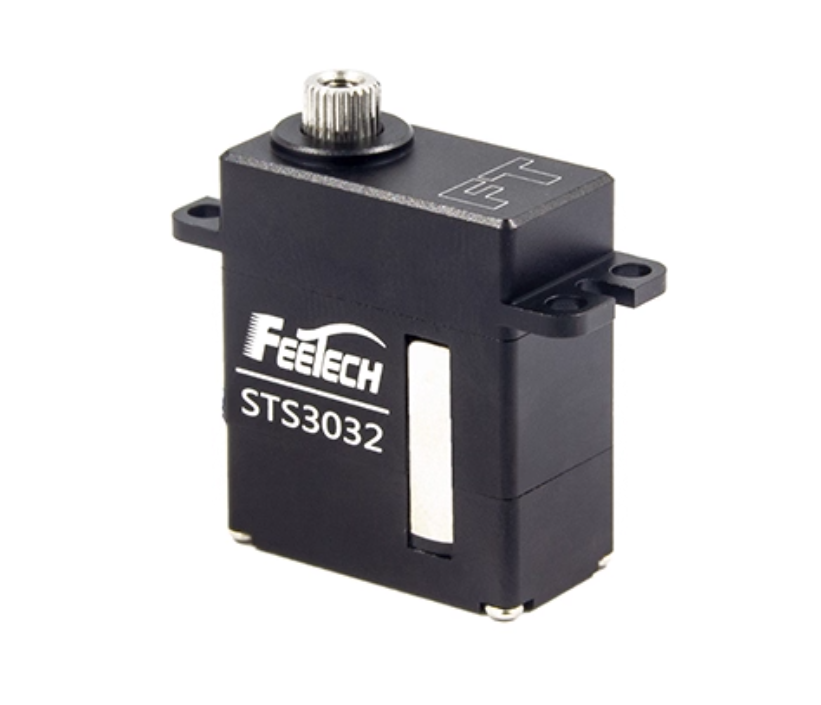
\includegraphics[width=0.7 \linewidth]{Figures/STS3032.png} 
    \caption{Feetech 3032 for output}
    \label{fig:81}
\end{figure}
For the input actuation, shown in Fig.\ref{fig:81}, the Feetech STS3009 servo was selected based on a different set of requirements. Weighing 40 grams and providing a stall torque of 0.3 Nm, this more powerful motor serves two essential functions in the input stage: it maintains mechanical equilibrium by resisting forces from the output tendons, thus offering a stable and responsive feel to the operator, and it helps filter out high-frequency physiological tremors or unintended jerks, ensuring that only deliberate commands are transmitted to the end-effector.
\begin{figure}[htbp]
    \centering
    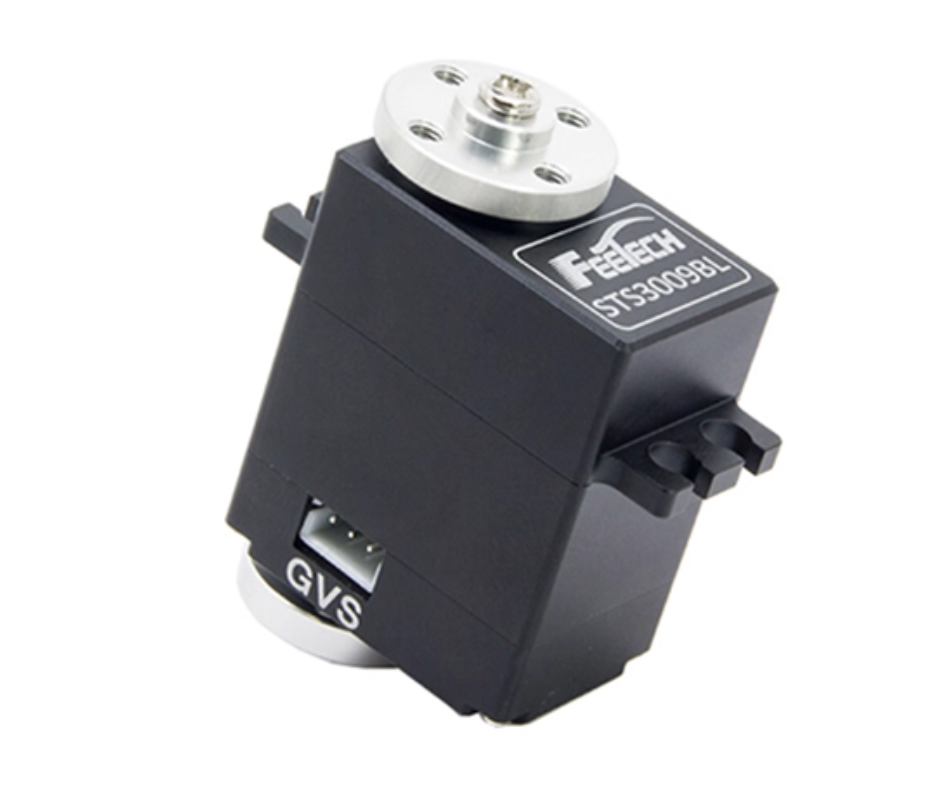
\includegraphics[width=0.7 \linewidth]{Figures/STS3009.png} 
    \caption{Feetech 3009 for wrist inputs}
    \label{fig:82}
\end{figure}


However, since the two input motors alone cannot fully capture all nuanced finger movements, a hybrid sensing strategy was implemented. Two AMS AS5600 magnetic rotary encoders were integrated into the input mechanism to directly and accurately detect the user’s intent. These sensors provide ultra-high 12-bit resolution and contactless sensing, enabling precise recognition of two distinct actions: the pinching gesture of the index finger and thumb, which controls grasping, and the rotational movement of the fingers, which is translated into in-plane rotation of the end-effector. This combination of robust actuation and high-resolution sensing creates an intuitive and stable human-machine interface suitable for delicate manipulation tasks.

\section{Cable Routing and Guidance System}
\subsection{Tip Design}
\begin{figure}[htbp]
    \centering
    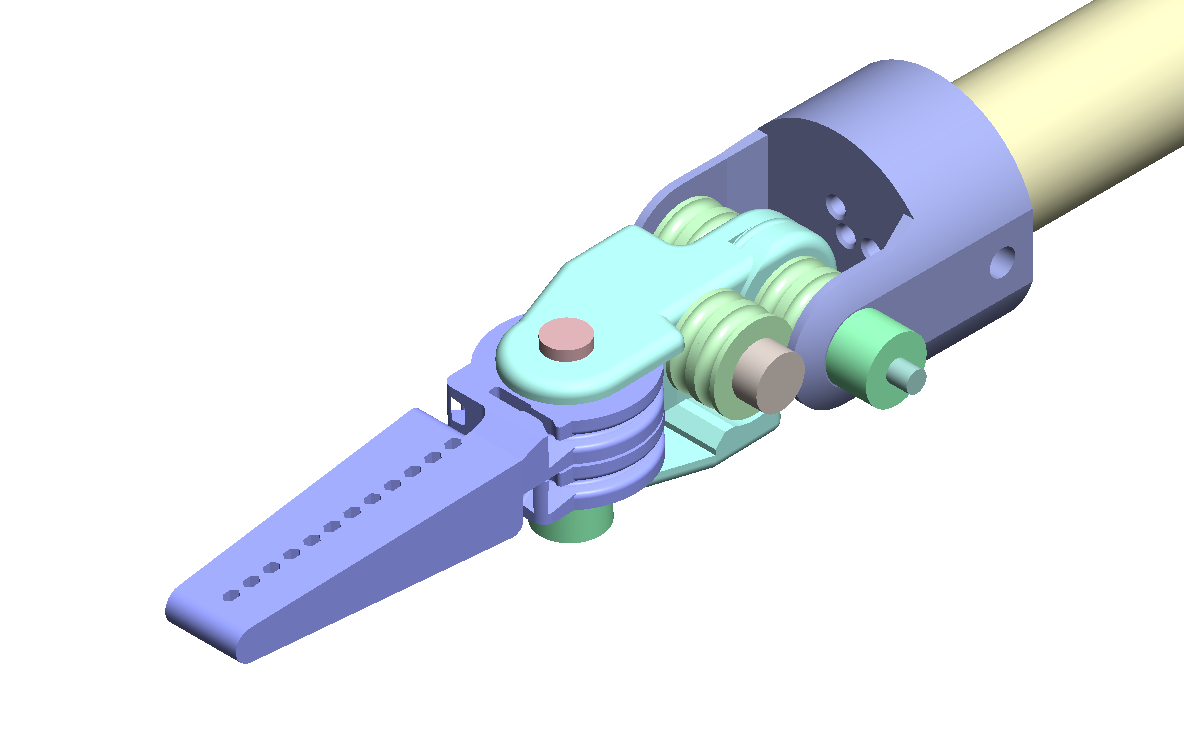
\includegraphics[width=0.7 \linewidth]{Figures/tip2.png} 
    \caption{Tip Design for Cable Guidance}
    \label{fig:83}
\end{figure}
In addition to motor performance, the accuracy and repeatability of the end-effector’s motion are highly dependent on precise cable guidance and sustained tension control. To ensure consistent behavior during operation, each cable must be constrained to move freely yet securely within a meticulously designed path, minimizing unwanted friction and slack.

A specialized tip assembly has been developed to fulfill these requirements. As shown in Fig.\ref{fig:83}, the four cables—grouped into two pairs, each controlling one jaw of the plier—are routed through custom-machined channels. These channels ensure that the cables remain aligned throughout the entire range of motion, avoiding cross-interference and reducing wear.

The two jaw components (fabricated in light pink) are mounted onto a central middle base (green). To further enhance cable stability and minimize friction, donut-shaped guides machined via CNC (purple) are integrated into the middle base. These spheres act as low-friction directional pulleys, maintaining cable position with high precision and reducing bending stress, thereby extending cable service life.

The main base housing (pink) is designed with precision-aligned holes that direct the cables perpendicularly toward the motors. This alignment is critical for maximizing force transmission efficiency and eliminating off-axis loading, which can introduce positioning errors and reduce system responsiveness.

Through this integrated approach—combining dedicated guiding channels, spherical contact points, and perpendicular alignment—the system achieves high repeatability, minimal hysteresis, and smooth force feedback, making it suitable for delicate manipulation tasks requiring fine motor control.

\subsection{Reel}

A fundamental challenge in cable-driven mechanisms lies in maintaining adequate tension during both winding and unwinding phases. In a conventional single-motor-single-cable configuration, unidirectional actuation presents a significant limitation: while rotation in one direction (e.g., clockwise) effectively pulls and tensions the cable, reverse rotation (counterclockwise) does not positively push the cable but often results in slack accumulation along the path. This leads to unpredictable response, reduced positional accuracy, and potential entanglements.

To address this issue, a paired-cable design has been implemented. The two cables corresponding to a single degree of freedom are affixed to the same axial shaft driven by one motor. This configuration effectively reforms the two independent cables into a continuous loop—functioning conceptually as a flexible drive belt. As a result, when the motor rotates in one direction, one cable is pulled while the other is simultaneously recovered, enabling bidirectional force transmission without slack accumulation.

\begin{figure}[htbp]
    \centering
    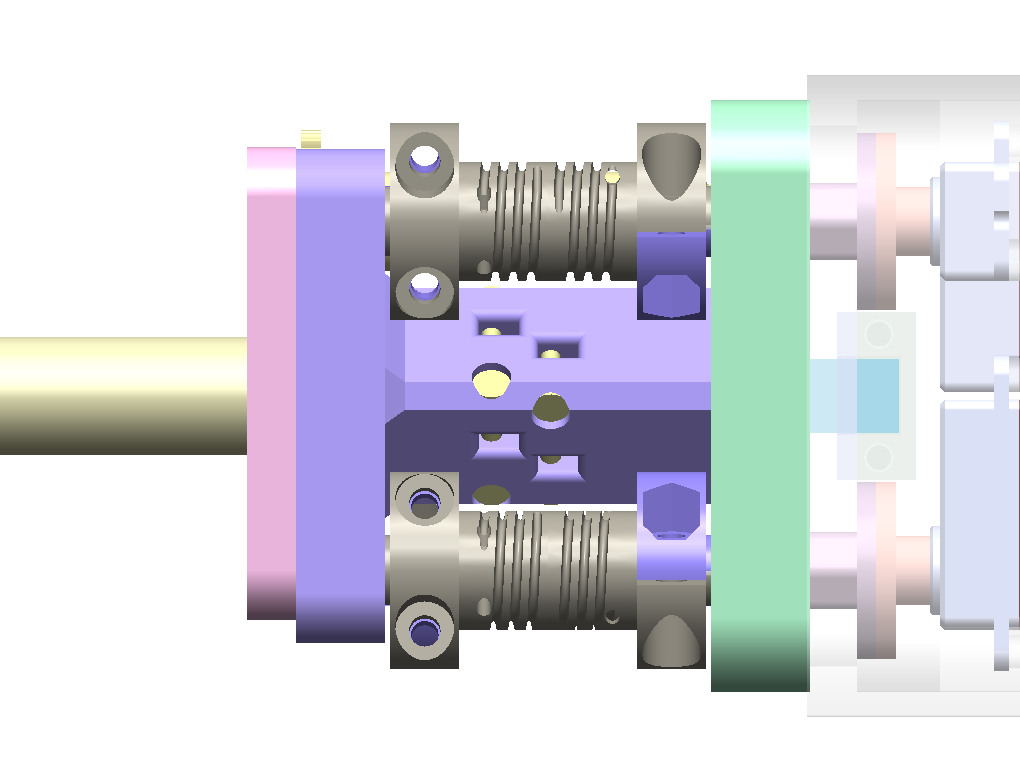
\includegraphics[width=0.7 \linewidth]{Figures/reel.png} 
    \caption{Reel Design and Winding Mechanism}
    \label{fig:84}
\end{figure}

The key to ensuring effective operation of this belt-like linkage is sustained cable tension. To achieve this, the reel assembly is split into two distinct components, each dedicated to one cable. These two reel pieces are mounted on the same shaft and are designed to rotate in opposite directions relative to each other. This counter-rotation ensures that one cable is wound while the other is unwound during actuation, maintaining constant tension across the system.

To prevent slippage and undesired loosening of the cables during operation, one-way bearings are incorporated into the reel mechanism. As the name implies, these bearings permit free rotation in one direction while locking in the opposite direction. This feature is critical for preserving tension integrity, especially during transitions in motor direction or under varying load conditions. The use of one-way bearings enhances system reliability, improves motion accuracy, and minimizes the need for manual tension adjustments.

\subsection{Motor Arrangement and Quick-Swap Mechanism}

As previously discussed, the STS3032 servos are employed as the driving motors for the cable reels. In practical surgical scenarios, various end-effector tips are often required throughout a single procedure. To accommodate this need, a quick-swap system has been integrated into the design, allowing for rapid and secure tip replacement without compromising system integrity.

To achieve a compact form factor suitable for handheld operation, the four motors are arranged in a rotational symmetry pattern within the main housing. This layout optimizes spatial efficiency while maintaining sufficient clearance for motor power and communication cables, thereby preventing interference and ensuring reliable connectivity.
\begin{figure}[htbp]
    \centering
    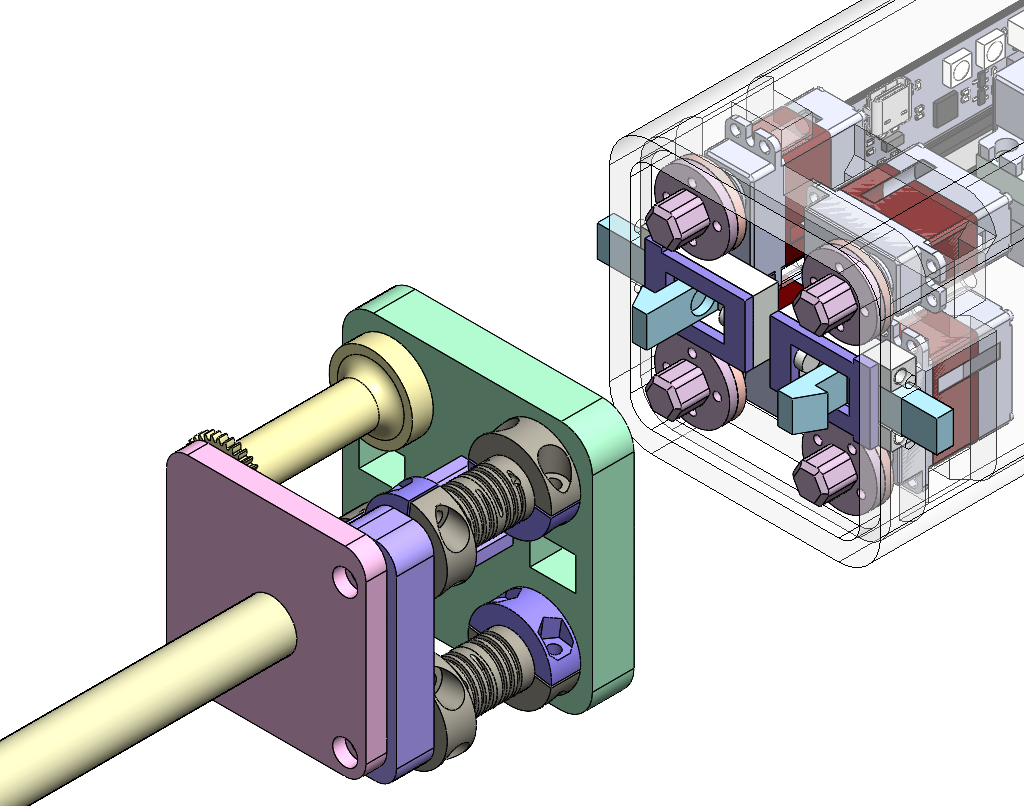
\includegraphics[width=0.7 \linewidth]{Figures/Motor Arrangement.png} 
    \caption{Motor Arrangement and Quick-Swap Mechanism}
    \label{fig:85}
\end{figure}
The quick-swap mechanism incorporates a user-friendly yet secure attachment scheme. Press-activated hooks are mounted within the main frame, enabling tool-free engagement and release. To attach a tip module, the user simply aligns and applies gentle pressure until the hooks audibly lock into place. For disengagement, bilateral release buttons must be depressed simultaneously while withdrawing the module. This dual-action release strategy prevents accidental detachment during operation, enhancing safety, while minimizing the number of steps required for module exchange.

This design ensures a robust mechanical and electrical connection during use, maintaining precise cable alignment and tension integrity while facilitating efficient tool interchange in time-sensitive surgical environments.

\subsection{Input Design}

The input module is designed to intuitively capture the user’s hand and finger motions with high precision and minimal latency. By integrating two STS3009 servos and two AS5600 magnetic encoders, the system is capable of sensing four degrees of freedom (DoFs): two DoFs from the wrist movement—yaw and pitch—and two DoFs from the fingers, namely roll and open/close actuation.

The wrist motions are translated through a dual-axis gimbal-like mechanism, where the STS3009 servos provide both actuation force and preliminary positional feedback. Fine rotational movements in yaw and pitch are accurately detected and relayed to the control system, enabling responsive and natural manipulation of the end-effector.
\begin{figure}[htbp]
    \centering
    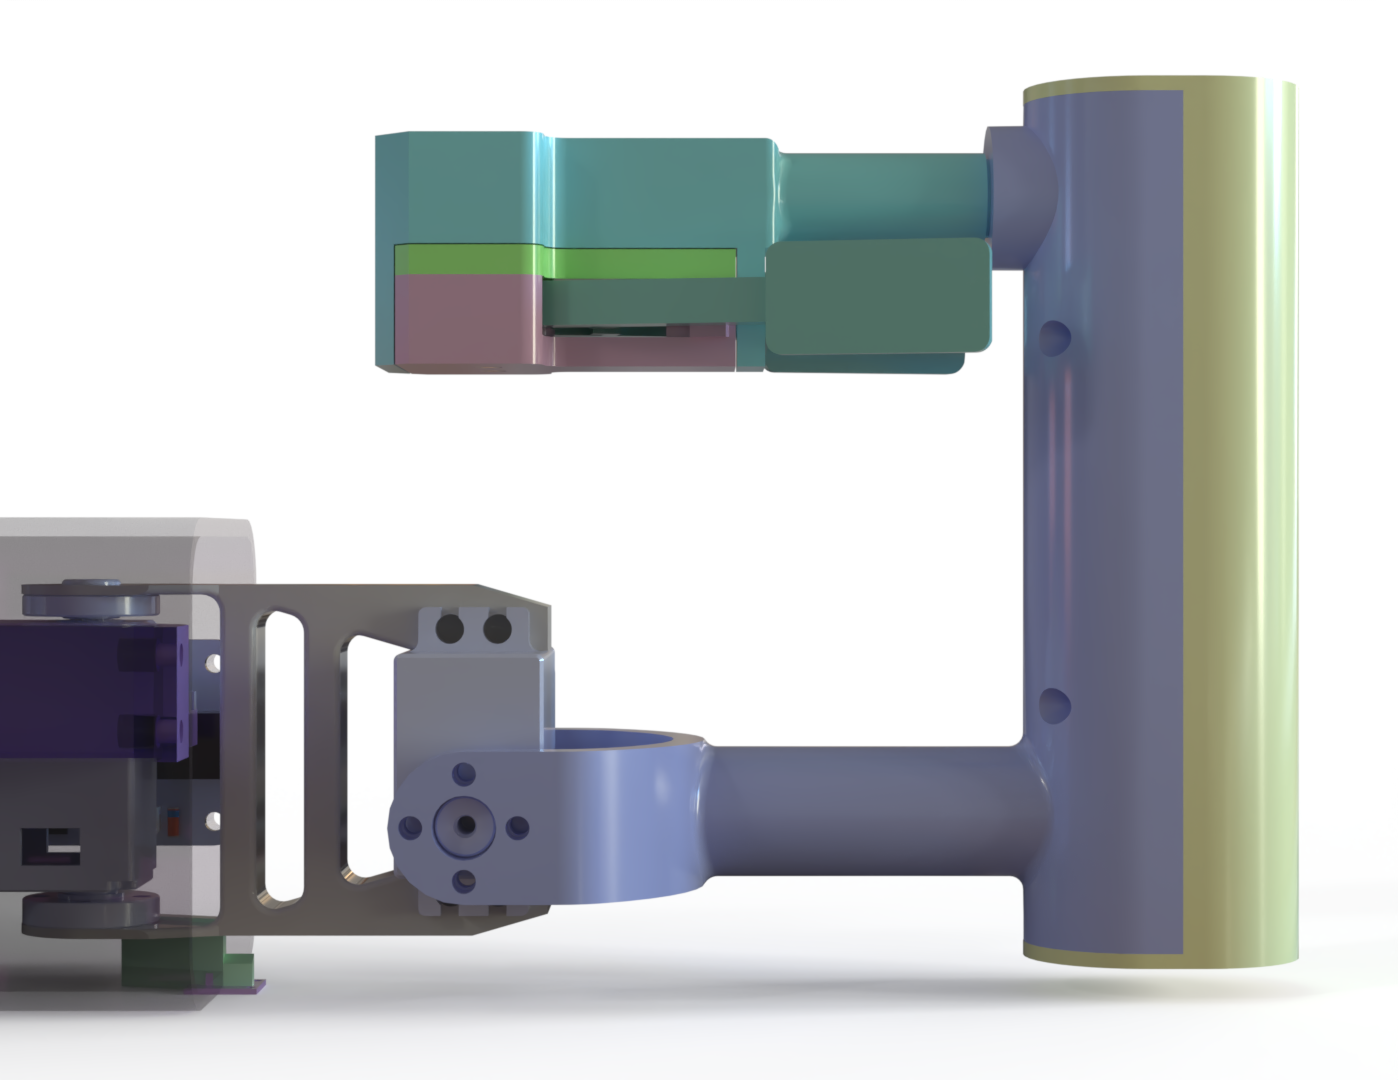
\includegraphics[width=0.7 \linewidth]{Figures/input.png} 
    \caption{Input Module Design}
    \label{fig:86}
\end{figure}
Finger actions are captured using the high-resolution AS5600 encoders, which detect both the rolling gesture and the degree of opening or closing of the fingers. Specifically, the open/close mechanism is implemented as an interchangeable module, allowing customization based on user preference or task requirements. The lever length and rebound force can be easily adjusted or swapped, facilitating ergonomic adaptability and reducing user fatigue during prolonged operations.

This modular and sensor-rich input design ensures that the system can accommodate a wide range of hand sizes and operating styles while maintaining accurate and reliable motion mapping between the user and the instrument.
%% Chapter Template

\section{Control Strategy} % Main chapter title

%\label{Chapter9} % Change X to a consecutive number; for referencing this chapter elsewhere, use \ref{ChapterX}\ref{ChapterX}\ref{ChapterX}\ref{ChapterX}

%----------------------------------------------------------------------------------------
%	SECTION 1
%----------------------------------------------------------------------------------------
\subsection{Digital Signal Logic}
A critical aspect of ensuring precise control of the end-effector tip is the ability to accurately interpret user intent while rejecting extraneous inputs, such as physiological tremor or unintended vibrations. To achieve this, an advanced signal processing and control architecture has been implemented.

An Extended Kalman Filter (EKF) is employed to fuse and filter raw data acquired from multiple sources, including the AS5600 encoders and the feedback from the STS3009 servos. The EKF provides robust state estimation by dynamically weighting sensor inputs and predicting true user motion in the presence of noise and transient disturbances. This results in smooth, stable, and intentional control signals that faithfully represent operator commands while effectively suppressing high-frequency noise and involuntary motions.

At the core of the control system is an ESP32 microcontroller, which serves as the central computation unit. This chip is responsible for executing the EKF algorithm in real-time, processing sensory data, generating corresponding motor commands, and managing communication between system components. Its high processing power and support for floating-point operations make it well-suited for handling computationally intensive filtering and control tasks onboard.

After the user's input signals are filtered and interpreted, the refined commands are transmitted to the output-stage STS3032 motors that drive the cables. To further enhance motion accuracy and disturbance rejection, a PID control strategy is implemented based on real-time feedback from the STS3032 motors' built-in encoders. This closed-loop architecture enables precise regulation of cable tension and position, providing haptic transparency and ensuring safe, responsive operation during delicate surgical tasks. The combination of high-level EKF-based intention recognition and low-level PID motor control creates a robust hierarchical control system capable of compensating for both environmental uncertainties and human factors.

\subsection{Human-Machine Interface}

The control signals are transmitted from the rear input motors to the front output motors, ultimately driving the tip of the instrument. However, the system operates without physical switches or buttons to initiate or terminate control. To address this, a specially designed sequence of actions is implemented to ensure safe and intuitive operation.

Since the smart servos are equipped with absolute magnetic encoders, and their rotational range is limited to less than 360 degrees, the initial position of each motor can always be reliably identified. Upon powering on the device, the four front motors automatically execute a homing sequence. This process ensures that all cables are brought to a known tension state before any user input is accepted, thereby preventing uncontrolled movements and ensuring system readiness.

User control is enabled only after the homing process is complete. Slight pressure applied to the input lever serves as the trigger to activate the control linkage. This intentional design requires a deliberate action from the user, minimizing the risk of accidental engagement.

To terminate control, the user simply releases the lever. This action locks the rear input motors, effectively decoupling the user's hand from the instrument tip. This not only enhances safety by preventing unintended motions but also allows the entire instrument to be repositioned as a rigid unit during surgical procedures without affecting the end-effector's configuration. This approach provides a seamless and secure method for transitioning between active manipulation and passive positioning.
%\include{Chapters/Chapter10}
%\include{Chapters/Chapter11}

%----------------------------------------------------------------------------------------
%	THESIS CONTENT - APPENDICES
%----------------------------------------------------------------------------------------

\appendix % Cue to tell LaTeX that the following "chapters" are Appendices

% Include the appendices of the thesis as separate files from the Appendices folder
% Uncomment the lines as you write the Appendices

%\include{Appendices/AppendixA}
%\include{Appendices/AppendixB}
%\include{Appendices/AppendixC}


%----------------------------------------------------------------------------------------
%	BIBLIOGRAPHY
%----------------------------------------------------------------------------------------

\printbibliography[heading=bibintoc]

%----------------------------------------------------------------------------------------

\end{document}
